\documentclass[11pt,a4paper]{report}
\usepackage[utf8]{inputenc}
\usepackage[pdftex]{graphicx} %for embedding images
\usepackage{url} %for proper url entries
\usepackage[bookmarks, colorlinks=false, pdfborder={0 0 0}, pdftitle={<pdf title here>}, pdfauthor={<author's name here>}, pdfsubject={<subject here>}, pdfkeywords={<keywords here>}]{hyperref} %for creating links in the pdf version and other additional pdf attributes, no effect on the printed document
%\usepackage[final]{pdfpages} %for embedding another pdf, remove if not required
\usepackage{amsmath}
\usepackage{calrsfs}
%\usepackage{mathabx}
\usepackage{listings}
\usepackage{titlesec}
\usepackage{lipsum}
\usepackage{tikz}
\usepackage{amsthm}
\usepackage{dsfont}
\usepackage{derivative}
\usepackage{marginnote}
\usepackage{amssymb}
\usepackage{siunitx}
\usepackage{gensymb}
\usepackage{mathrsfs}
\usepackage{physics}



\usetikzlibrary{shapes.geometric, arrows}
\tikzstyle{startstop} = [rectangle, rounded corners, minimum width=3cm, minimum height=1cm,text centered, draw=black, fill=red!30]
\tikzstyle{io} = [trapezium, trapezium left angle=70, trapezium right angle=110, minimum width=3cm, minimum height=1cm, text centered, draw=black, fill=blue!30]
\tikzstyle{process} = [rectangle, minimum width=3cm, minimum height=1cm, text centered, draw=black, fill=orange!30]
\tikzstyle{decision} = [diamond, minimum width=3cm, minimum height=1cm, text centered, draw=black, fill=green!30]
\tikzstyle{arrow} = [thick,->,>=stealth]
\usepackage{geometry}
 \geometry{
 a4paper,
 total={170mm,257mm},
 left=20mm,
 top=20mm,
 }
\usepackage{mathtools}
\DeclarePairedDelimiter\ceil{\lceil}{\rceil}
\DeclarePairedDelimiter\floor{\lfloor}{\rfloor}
\usepackage{fancyhdr}
\setlength{\headheight}{14.49998pt}
\pagestyle{fancy}
\fancyhf{}
\rhead{\thepage}
\lhead{Dissertation Report}
\lfoot{Suprio Dubey}
\rfoot{2013036}

\usepackage{listings}
\usepackage{color}
 
\lstdefinestyle{mystyle}{
    backgroundcolor=\color{white},   
    commentstyle=\color{green},
    keywordstyle=\color{red},
    numberstyle=\tiny\color{gray},
    stringstyle=\color{blue},
    basicstyle=\footnotesize,
    breakatwhitespace=false,         
    breaklines=true,                 
    captionpos=b,                    
    keepspaces=true,                 
    numbers=left,                    
    numbersep=5pt,                  
    showspaces=false,                
    showstringspaces=false,
    showtabs=false,                  
    tabsize=2
}
 
\lstset{style=mystyle}
\usepackage[absolute,overlay]{textpos}
\usepackage[document]{ragged2e}
\usepackage[toc,page]{appendix}
\usepackage{imakeidx}
\usepackage{hyperref}
\makeindex
%\newcommand{\lambdabar}{{\mkern0.75mu\mathchar '26\mkern -9.75mu\lambda}}
 


\begin{document}

\begin{titlepage}
\begin{center}

% Title
\vspace*{.2in}
\parbox{\textwidth}{\centering
\huge \textbf {Extracting cosmological information at non-linear scales using machine learning}
}\\[.2in]

% Submitted by
\Large Submitted by \\
\vspace{.1in}
\Large \textbf{Suprio Dubey}\\
\textbf{(2013036)}\\[.5in]

% Center bottom of the page

\includegraphics[width=0.5\textwidth]{logo.jpg}\\[0.5in]
\Large{Department of Physics and Astronomy}\\
\normalsize
\textsc{University of Padua}\\
Padua, Italy \\
\vspace{0.2cm}

\vfill

% Supervisor and Co-supervisor
\vspace{\fill}
\hfill
\begin{minipage}{0.4\textwidth}
    \raggedleft % Align text to the right
    \large
    \textbf{Supervisor:}\\
    Michele Liguori\\
    \vspace{0.2cm}
    \textbf{Co-Supervisors:}\\
    Andrea Ravenni, Gabriel Jung
\end{minipage}
 

\end{center}
\end{titlepage}



\pagenumbering{roman}
\newpage
\begin{center}
    \huge \textbf{Abstract}
\end{center}

\vspace{0.5in}

One of the most sought unanswered questions in cosmology is what is Dark Matter? Dark Matter is thought to account for approximately $ 85\%$ of the matter contained in the universe and yet the exact nature of it is still unknown.  In 1971 it was proposed by Hawking\cite{1971MNRAS.152...75H} that a highly overdense region in the primordial universe could undergo gravitational collapse directly to form black holes.  Primordial Black Holes(PBH), are thought to be one of the potential candidates for dark matter as they form before matter-radiation dominated equality, hence they are non-baryonic. This makes them an intriguing subject for research. Large perturbations that exit the horizon during inflation may result in the formation of PBH. The recent gravitational waves (GWs) detection of tens of solar  masses black hole binaries by the LIGO-Virgo collaboration has stoked interest in PBH as a dark matter. \\
The literature on PBH is reviewed in this dissertation. A brief explanation of the observational evidence and the dynamics of dark matter are included in Chapter 1 along with several essential cosmological concepts. We analyze the flaws in the conventional cosmological model and how inflation addresses them in Chapter 2. We will also talk about how quantum fluctuations brought on by inflation can result in PBH formation. The development of PBH, its abundance, the shortcomings of the simplified model and a brief discussion of the inflationary theories used to generate it will all be covered in Chapter 3. The summary of the observational constraints on the PBH mass function will follow as our final point.
\tableofcontents




\pagenumbering{arabic}

\chapter{Introduction}
\section{The Center of the Universe}

One of the foundations of modern cosmology is the Cosmological Principle. If we view it over a large scale, the universe is independent of the position i.e $homogeneous$, and independent of direction i.e $isotropic$ to a first approximation.
The spacetime geometry that is consistent with the universe being homogeneous and isotropic is given by the Friedmann-Roberston Walker Metric(FRW) metric.
\begin{align}
     ds^2= -c^2dt^2 + a(t)^2\left(\frac{dr^2}{1-\kappa r^2}+ r^2d\theta^2 +r^2sin^2\theta d\phi^2\right )\label{eq:1.1}
\end{align}\\
where $k = 0$, $k = +1$ and 
$k = -1$ for flat, positively curved and negatively curved spacelike $3$---hypersurfaces, respectively. Whereas, $a(t)$ is the scale factor that incorporates the expansion of the universe. For ease of notation, we will restrict most of our discussion to the case $k = 0$.
\hspace{0.5cm}\\
We can write the FRW metric in the flat space i.e. taking the form of the Minkowski metric with the scale factor.

\begin{align}
    d{s^2} = -\ d{t^2} + a^2(t) \ d{\sigma^2}\label{eq:1.2}
\end{align}\\
where 
\begin{align}
     d{\sigma^2} = \gamma_{ij} \ d{x^{i}} \ d{x^{j}}\label{eq:1.3}
\end{align}\\
with 
\begin{align}
    \gamma_{ij}= \delta_{ij} + \kappa\frac{x_{i}x_{j}}{1-\kappa(x_k x^k)}\label{eq:1.4}
\end{align}\\
\hspace{0.5cm}We can notice that by using the polar coordinates we can  get to equation \ref{eq:1.1}. The polar coordinate used in the equation \ref{eq:1.1} refers to the observer comoving with the expansion of the universe. We get the physical distance by multiplying the moving distance with the scale factor.\\
We can redefine the radial coordinate as  
\begin{align}
    d\chi = \frac{dr}{\sqrt{1-\kappa r^2}}\label{eq:1.5}
\end{align}\\
such that,
\begin{align}
   ds^2= -dt^2 + a(t)^2\left[{d\chi^2}+ f(\chi)^2(d\theta^2 +sin^2\theta d\phi^2)\right ]\label{eq:1.6}
\end{align}\\
where,
\begin{align}
    f(\chi) = \begin{cases}
        sinh\chi,& \kappa=-1\\
        \chi,& \kappa=0\\
        sin\chi,& \kappa=+1
    \end{cases}
\end{align}\\
This form of metric is particularly convenient for studying the propagation of light. Light travels along the null geodesic $ds^2=0$ so to make the propagation of light in FRW similar to the Minkowski space we introduce conformal time,
\begin{align}
    d\tau = \frac{dt}{a(t)},\label{eq:1.8}
\end{align}\\
Substituting it in \ref{eq:1.6} we get 
\begin{align}
    ds^2= -a(\tau)^2\left[d\tau^2 - \left({d\chi^2}+ f(\chi)^2(d\theta^2 +sin^2\theta d\phi^2)\right)\right ]\label{eq:1.9}
\end{align}
    
\section{Freidmann Equation}
\hspace{0.5cm}The dynamics of the way the universe evolves are determined by the Einstein equation.
\begin{align}
    G_{\mu \nu } = R_{\mu \nu } - \frac{1}{2} g_{\mu \nu } R = 8 \pi G T_{\mu \nu }\label{eq:1.10}
\end{align}\\
This relates to the Einstein tensor $G_{\mu \nu }$ which is a measure of the “space-time curvature” of the FRW
universe to the stress-energy tensor where $T_{\mu \nu }$ is the measure of the “matter content” of the universe.\\

\subsection{Space-time Curvature}
\hspace{0.5cm}Let us compute the Einstein tensor on the l.h.s. of the Einstein equation $G_{\mu \nu } = R_{\mu \nu } - \frac{1}{2} g_{\mu \nu } R$ \\ 
The Ricci tensor is given by :
\begin{align}
        R_{\mu \nu } = \Gamma^{\alpha }_{\mu \nu , \alpha } 
        - \Gamma^{\alpha }_{\mu \alpha , \nu }
        + \Gamma^{\beta }_{\mu \nu } \Gamma^{\alpha }_{\alpha \beta } 
        - \Gamma^{\beta}_{\mu \alpha } \Gamma^{\alpha }_{\nu \beta }
\end{align}
Let us see the Christoffel symbols for the FRW metric:\label{1.12}
%\begin{claim}
\begin{subequations}
    \begin{align}
        %\begin{gather}
            \Gamma^{0}_{\mu \nu } &= \left[\begin{array}{cccc}
            0 & 0 & 0 & 0 \\ 
            0 & \frac{\dot{a}a}{1-kr^2} & 0 & 0 \\ 
            0 & 0 & r^2a \dot{a} & 0 \\ 
            0 & 0 & 0 & r^2 a \dot{a} \sin^2\theta 
            \end{array}\right]\label{eq:1.12a} \\
            \Gamma^{1}_{\mu \nu } &= \left[\begin{array}{cccc}
            0 & \dot{a} / a & 0 & 0 \\ 
            \dot{a} / a & \frac{kr}{(1-kr^2)} & 0 & 0 \\ 
            0 & 0 & (kr^2-1)r & 0 \\ 
            0 & 0 & 0 & (kr^2-1)r \sin^2\theta 
            \end{array}\right] \label{eq:1.12b}\\ 
            \Gamma^{2}_{\mu \nu } &= \left[\begin{array}{cccc}
            0 & 0 & \dot{a} / a & 0 \\ 
            0 & 0 & 1 / r & 0 \\ 
            \dot{a} / a & 1/r & 0 & 0 \\ 
            0 & 0 & 0 & - \sin \theta \cos \theta 
            \end{array}\right]\label{eq:1.12c} \\ 
            \Gamma^{3}_{\mu \nu } &= \left[\begin{array}{cccc}
            0 & 0 & 0 & \dot{a} / a \\ 
            0 & 0 & 0 & 1/r \\ 
            0 & 0 & 0 & \cos \theta  /\sin \theta  \\ 
            \dot{a} /a  & 1/r & \cos \theta  /\sin \theta  & 0
            \end{array}\right] \label{eq:1.12d}\\ 
        %\end{gather}
    \end{align}
\end{subequations}
%\end{claim}
   

Here we used simplifications that the FRW metric is diagonal, and it does not depend on \(\varphi \).\\

The components of the Ricci tensor are: 
    
\begin{subequations}
    \begin{align}
        R_{00} & = - 3 \partial_{t} (\frac{\dot{a}}{a})  - 3 (\frac{\dot{a}}{a})^2\\
        & = -3 \left(\frac{\ddot{a}}{a} - (\frac{\dot{a}}{a})^2 + (\frac{\dot{a}}{a})^2\right)\\ 
        & = - 3 \frac{\ddot{a}}{a}
    \end{align}
\end{subequations}
    


    
\begin{subequations}
    \begin{align}
        \begin{split}
            R_{11} &= \partial_{t} (\frac{\dot{a} a}{1 - kr^2} )
            + \partial_{r} (\frac{kr}{1 - kr^2})
            - \partial_{r} (\frac{kr}{1 - kr^2})
            - 2 \partial_{r} (\frac{1}{r}) \\
            &\phantom{=}\ 
            + \frac{\dot{a} a}{1 - kr^2} 3 \frac{\dot{a}}{a}
            + \frac{kr}{1-kr^2} (\frac{kr }{1 - kr^2} + \frac{2}{r}) \\
            &\phantom{=}\ 
            - 2 \frac{\dot{a}}{a} \frac{\dot{a} a}{1 - kr^2}
            - (\frac{kr}{1 - kr^2})^2 
            - 2 (\frac{1}{r})^2
        \end{split}  \\
        &= \frac{\ddot{a} a + \dot{a}^2}{1 - kr^2} 
        + 3 \frac{\dot{a}^2}{1 - kr^2}
        + 2 \frac{k}{1 - kr^2}
        - 2 \frac{\dot{a}^2}{1 - kr^2}  \\
        &= \frac{\ddot{a} a + 2 \dot{a}^2 + 2 k}{1 - kr^2}
    \end{align}
\end{subequations}
    
\begin{subequations}
    \begin{align}
        \begin{split}
            R_{22} &= 
            r^2 \partial_{t} (a \dot{a})
            + \partial_{r} ((kr^2-1)r)
            - \partial_{\theta } (\frac{\cos \theta }{\sin \theta }) \\
            &\phantom{=}\ 
            +3 \Gamma^{t}_{\theta \theta } \Gamma^{\theta }_{t \theta } + \Gamma^{r}_{\theta \theta } (\Gamma^{r}_{r r } + 2 \Gamma^{\theta }_{r \theta })
            -2 (\Gamma^{t}_{\theta \theta } \Gamma^{\theta }_{t \theta } + \Gamma^{r}_{\theta \theta } \Gamma^{\theta }_{\theta r}) - \frac{\cos^2 \theta}{\sin^2\theta }
        \end{split}  \\
        &= r^2 (\ddot{a} a + \dot{a}^2)
        + 3kr^2 - 1 + \frac{1}{\sin^2\theta} 
        +  r^2 \dot{a}^2
        - kr^2
        - \frac{\cos^2\theta }{\sin^2\theta }  \\
        &= r^2 (\ddot{a} a + 2\dot{a}^2 + 2k)
    \end{align} 
\end{subequations}

\begin{subequations}
    \begin{align}
        R_{33} &= \partial_{\alpha } \Gamma^{\alpha }_{\varphi \varphi } - \partial_{\varphi } \Gamma^{\alpha }_{\alpha \varphi } + \Gamma^{\alpha }_{\varphi \varphi } \Gamma^{\beta }_{\alpha \beta } - \Gamma^{\beta }_{\varphi \alpha } \Gamma^{\alpha }_{\varphi \beta }  \\
        &= r^2 \sin^2\theta (\ddot{a} a + 2 \dot{a}^2 + 2k) 
    \end{align}
\end{subequations}


The Ricci scalar then comes out to be 

\begin{subequations}
    \begin{align}
        \begin{split}
            R = g^{\mu \nu } R_{\mu \nu } 
            &= 3 \frac{\ddot{a}}{a} 
            + \frac{1-kr^2}{a^2} \frac{\ddot{a}
             a + 2 \dot{a}^2 + 2k}{1 - kr^2} \\
             &\phantom{=}\ 
            + \frac{1}{a^2r^2} r^2 (\ddot{a} a + 2 \dot{a}^2 + 2k)
            + \frac{1}{a^2r^2 \sin^2\theta }
            r^2 \sin^2\theta  (\ddot{a} a + 2 \dot{a}^2 + 2k) 
        \end{split}
        \\
        &= 3 \frac{\ddot{a}}{a} + 3 \frac{\ddot{a}a + 2 \dot{a}^2 + 2k}{a^2}
        \\
        &= 6 \left[\frac{\ddot{a}}{a} + (\frac{\dot{a}}{a}) + \frac{k}{a^2}\right]
        \,.
    \end{align}
\end{subequations}

We find that the non-zero components of the Einstein tensor $G^{\mu}_{\nu} = g^{\mu \lambda}G_{\lambda \nu }$
\begin{subequations}
    \begin{align}
        G^{0}_{0} = 3 \left[\left(\frac{\dot{a}}{a}^2\right) + \frac{k}{a^2}\right]\label{eq:1.18a}
    \end{align}
    \begin{align}
        G^{i}_{j} =  \left[2\frac{\ddot{a}}{a} + \left(\frac{\dot{a}}{a}^2\right) + \frac{k}{a^2}\right]\delta^{i}_{j}\label{eq:1.18b}
    \end{align}
\end{subequations}
\hspace{0.5cm}\\

*\subsection{Stress-energy Tensor}
\hspace{0.5cm}For the universe to be isotropic and homogeneous it is forced to be a perfect fluid. Perfect fluids have a stress-energy tensor like :
\begin{align}
    T^{\mu \nu } =  (\rho + P) u^{\mu } u^{\nu } + P g^{\mu \nu }\label{eq:1.19}
\end{align}\\

where $u^{\mu }$ is the 4-velocity of the fluid element. It is diagonal in the $\emph{comoving frame}$, in which $u^{\mu } = (1, \vec{0})$.\\
\hspace{0.5cm}If we take the covariant divergence of the Einstein tensor \(G_{\mu \nu }\) we get zero; so the stress-energy tensor must also have \(\nabla_{\mu} T^{\mu \nu }=0\). 
One key emphasis here is that the covariant derivative of the stress-energy tensor is not a conservation equation unlike in special relativity where the equation  \(\partial_{\mu}  T^{\mu \nu }\) describes a conservation equation, a local one.\\ 
\hspace{0.5cm}In GR we get a conserved quantity if the metric doesn't depend on some coordinate ($\equiv$ something constant). 
We denote Killing Vectors, a vector oriented in the direction of symmetry. But in cosmology, we do not have symmetry with respect to time translation, so there is no time-like Killing vector \(\xi_{\mu }\) such that \(\xi_{\nu } \nabla_{\mu } T^{\mu \nu }\) represents the conservation of energy.\\
This equation, \(\nabla_{\mu } T^{\mu \nu }\) follows from the fact that our fluid follows its equations of motion. 
Let us explore the meaning of these equations. If, in the equation \( \nabla_{\mu } T^{\mu}_{0} = 0\),  we find 
\begin{subequations}
    \begin{align}
        \nabla_{\mu } T^{\mu}_{0} 
        &= \partial_{\mu } T^{\mu }_{0} + \Gamma^{\mu }_{\mu \lambda } T^{\lambda }_{0} - \Gamma^{\lambda }_{\mu 0} T^{\mu }_{\lambda }
        = 0 
    \end{align}
    \begin{quote}
        the term $T^{i}_{0}$ vanishes by isotropy. So we get,
    \end{quote}
    \begin{align}
        \partial_{t} \rho + \Gamma^{\mu }_{\mu 0} \rho - \Gamma^{\lambda }_{\mu 0} T^{\mu }_{\lambda } = 0 
    \end{align}
    \begin{quote}
        From \ref{eq:1.12b},\ref{eq:1.12c},\ref{eq:1.12d} we see that $\Gamma^{\lambda }_{\mu 0}$ vanishes
        unless $\lambda$ and $\mu$ are spatial indices equal to each other, in which case it is $\frac{\dot{a}}{a}$.The above equation therefore reads :
    \end{quote}
    \begin{align}
        \dot{\rho} + 3 \frac{\dot{a}}{a}(\rho + P) = 0 \label{eq:1.20c}
    \end{align}
\end{subequations}
To find the other two Friedmann equations we compare the time-time equation and the space-space equation of the Einstein equations to the stress-energy tensor i.e comparing \ref{eq:1.19} to \ref{eq:1.18a} and \ref{eq:1.18b} respectively
To relate the sources of matter to the evolution of the scale factor in the FRW metric \ref{eq:1.9}, 
\begin{subequations}
    \begin{align}
        \frac{\ddot{a}}{a} &= - \frac{4 \pi G}{ 3} (\rho + 3 P) \label{eq:1.21a}  \\
        \left(\frac{\dot{a}}{a}\right)^2 &= \frac{8 \pi G}{3} \rho - \frac{k}{a^2} \label{eq:1.21b}
    \end{align}
\end{subequations}\\
The space-space equation is not a dynamical equation, since it contains no second-time derivatives: it is a \emph{constraint} on the evolution of the system. 
However, the three Friedmann equations are not independent: the time-time one can be found from \ref{eq:1.21a} and \ref{eq:1.20c}.\\
We define $\left(\frac{\dot{a}}{a}\right) \equiv H $, the Hubble parameter which is the measure of the expansion rate of the universe, measured in $Km.s^{-1}.Mpc^{-1}$.\\ 
\hspace{0.5cm}The above equations \ref{eq:1.20c},\ref{eq:1.21a},\ref{eq:1.21b} describe how the universe expands and lay the groundwork for all further discussion of cosmology.
We can solve the Friedmann equations by an equation of state that relates $\rho$ to $P$. 
\begin{align}
    w = \frac{P}{\rho} . 
\end{align}
Plugging it in the continuity equation \ref{eq:1.20c} we get:
\begin{align}
    \frac{ \log \rho}{ \log a} = {-3(1 + w)} \implies \rho \propto a^{-3(1 + w)}\label{eq:1.23} 
\end{align}\\

\begin{align}
    \rho(a) \propto 
    \begin{cases}
        a^{-4} ,& \text{radiation: }  w =\frac{1}{3}\\
        a^{-3},              & \text{matter: }  w = 0\\
        constant,              & \text{dark energy: }  w = -1\\
    \end{cases}\label{eq:1.24}
\end{align}
It makes intuitive sense that the energy density of relativistic particles decreases as the universe expands, not only because the average number of particles per unit volume decreases ($V \propto a^3$), as it does for non-relativistic matter, but also because of the relativistic Doppler shift, which increases the negative power of the scaling factor by one. 
In contrast, dark energy has a constant energy density. 
We can assume that if the Universe is made up of those three types of fluids, then at different times, radiation, followed by matter, and finally Dark Energy, has dominated its energy budget and consequently its evolution.\\
Now, combining \ref{eq:1.23} with the first Friedmann equation \ref{eq:1.12b} we get the time dependence of the scale factor.
\begin{align}
    a(t) \propto 
    \begin{cases}
        t^{\frac{2}{3(1+w)}} ,& \text{if,}  w\neq -1\\
        e^{Ht},               & \text{if,}  w = -1\\
    \end{cases}\label{eq:1.25}
\end{align}\\
We can observe that for $w = 0$, which corresponds to a Universe dominated by non-relativistic matter, we get $a(t) \propto  t^{2/3}$. 
Now, for $w = 1/3$, which corresponds to relativistic particles (radiation), we get $a(t) \propto  t^{1/2}$. 
The last and very relevant case is $w = -1$, corresponding to a fluid exerting negative pressure, which leads to the second solution in \ref{eq:1.25}, i.e. an exponential expansion describes the Dark Energy.





\section{The Cosmological Constant}
\hspace{0.5cm}When Einstein developed his theory of general relativity, the prevailing belief was that the Universe was static. However, this contradicted the Friedmann equations, which showed that a Universe
evolving according to them could not be static unless the acceleration  $\vec{a}$ was zero. namely
\begin{align}
   \rho=-3 P \label{1.26}
\end{align}
Since a fluid with such property did not seem to be physically reasonable, Einstein modified equation \ref{eq:1.10} by introducing the cosmological constant term $\Lambda$ to counterbalance the gravitational attraction
\begin{align}
    R_{\mu \nu}-\frac{1}{2} g_{\mu \nu} R=8 \pi G T_{\mu \nu}-\Lambda g_{\mu \nu},\label{1.27}
\end{align}
 in such a way that it does not change the covariant character of the equations. It can be shown that for an appropriate choice of $\Lambda$, one indeed obtains a static cosmological model.
In order to recover a form similar to the equations \ref{eq:1.10}, we rewrite the stress-energy tensor in a more compact way

\begin{align}
    \bar{T}_{\mu \nu} & =T_{\mu \nu}-\frac{\Lambda}{8 \pi G} g_{\mu \nu} \\ & =(\bar{P}+\bar{\rho}) u_\mu u_\nu+\bar{P} g_{\mu \nu}, \label{1.29}
\end{align}

so that
\begin{align}
    R_{\mu \nu}-\frac{1}{2} g_{\mu \nu} R=8 \pi G \bar{T}_{\mu \nu}\label{1.30}
\end{align}


In \ref{1.29}, the effective pressure $\bar{P}$ and the effective density $\bar{\rho}$ are related to the corresponding quantities for a perfect fluid by
\begin{align}
    \bar{P}=P-\frac{\Lambda}{8 \pi G}, \quad \bar{\rho}=\rho+\frac{\Lambda}{8 \pi G}\label{1.31}
\end{align}

Although after the discovery of the expansion of the Universe in the late 1920s, there was no need for a term that made the Universe static, the cosmological constant remained a subject of great interest and it is today the simplest possible explanation for the observed accelerated expansion of the Universe. The standard model of cosmology that incorporates the effects of the cosmological constant is the $\Lambda$CDM model.

One cosmological model that involves the cosmological constant is the de Sitter Universe. In this model, the Universe is dominated by a positive cosmological constant, which suppresses all other matter contributions, making the Universe empty ($\rho=0$),($P = 0$) and flat ($k=0$). Under these conditions, the effective pressure and density are related to the cosmological constant through equation \ref{1.31} we get,
\begin{align}
   \bar{P}=-\bar{\rho}=-\frac{\Lambda}{8 \pi G}, \label{1.32}
\end{align}

which, if replaced in equation \ref{eq:1.21b} gives
\begin{align}
    \frac{\dot{a}^2}{a^2}=H^2=\frac{\Lambda}{3},\label{1.33}
\end{align}

corresponding to a Hubble parameter constant in time.The solution to
this equation is an exponential expansion, where the scale factor increases as a function of time
\begin{align}
    a \propto \exp \left(\sqrt{\frac{\Lambda}{3}} t\right),\label{1.34}
\end{align}


This exponential expansion means that test particles move away from
each other due to the repulsive gravitational effect of the positive cosmological constant.
In modern cosmology, $\Lambda$, the energy density $\rho_{\Lambda}$ and pressure $P_{\Lambda}$ is interpreted as the energy density and pressure of the vacuum, which is the ground state of a quantum system. Although the vacuum state does not
contain any physical particles, it is characterized by the creation and annihilation of virtual particles, which contributes to the total energy of the system with non-zero vacuum energy









\section{Cosmic Distances}\footnote{c = 1} 
In this section, we will introduce some useful quantities commonly used in cosmology. The Universe is observed to be expanding, and the scale factor $a(t)$ is increasing with time. This expansion also affects the photons that were emitted a long time ago far away and reach us today, which become redshifted due to the stretching of space. Therefore, it is convenient to define a quantity that describes the distance - and time - of a patch of the Universe we are observing based on this physical effect. For that, we define the redshift $z$ as
\begin{align}
    z+1 = \frac{a(t0)}{a(t)}
\end{align}
where $t$ is the time when the signal was emitted and $t_0$ is today. The scale factor is defined up to a multiplicative constant, and it's usually assumed $a(t_0) = 1$, so $z + 1 = a(t)^{-1}$.
As we know, the causal connection of points in space-time is determined by whether they are inside or outside each other's lightcone. Lightcones are the solutions to the equation
\begin{align}
ds^2 = 0,
\end{align}
where $ds^2$ is the space-time interval between two events. In other words, the lightcone of an event consists of all the events that could potentially receive a signal from the first event, assuming the signal travels at or below the speed of light. Any event inside the past lightcone of another event can be causally influenced by it, while any event outside the future lightcone cannot be influenced by it.
With $ds^2$ a suitable metric, in our case the FRW metric \ref{eq:1.6}, assuming a homogeneous and isotropic Universe and taking $d\Omega=0$,the comoving particle horizon is then, 
\begin{align}
    r_p(t) \equiv \chi(t) = \int_0^t \frac{ dt'}{a(t')} =  \int_0^a d\ln{a}\left(\frac{1}{aH}\right) = \tau \label{eq:1.28}
\end{align}

where in the last equality we exploited the relation we found earlier for the conformal time  Eq. \ref{eq:1.8}\footnote{The main benefit of working with conformal time: light rays correspond to straight lines at $45 \degree$ angles in the $\chi - \tau$ coordinates. If instead, we had used physical time t, then we would find the light cones for curved space-times would be curved.}.

The comoving horizon is therefore the logarithmic integral of the comoving Hubble radius $\frac{1}{aH}$, which we will define below. The related physical particle horizon is
\begin{align}
    d_p(t) = a(t) r_p(t) = a(t) \int_0^t \frac{ dt'}{a(t')} \label{eq:1.29}
\end{align}

due to the scale factor in the denominator and the fact that $a(t) \rightarrow 0$ as $t$ goes to 0, the particle horizon could become infinite, meaning that an observer would be in causal connection with the whole Universe. Using eq \ref{eq:1.25}, we can find an approximate expression for $d_p(t)$ for $w > -1/3$, or else we can notice that the integral diverges. Using the Hubble parameter in FRW model which is 
\begin{align}
    H = \frac{2}{3(1+w)t}
\end{align}
 With $w = 0$, a spatially flat matter-dominated universe, $H = 2/3t$ and $a \propto  t^ {\frac{2}{3}}$. With $w = 1/3$, a spatially flat radiation-dominated universe, we have $H = 1/2t$ and $a \propto  t^ {\frac{2}{3}}$.
we can write eq \ref{eq:1.29} as

\begin{align}
d_p(t) \simeq \frac{3(1+w)}{1+3w}t = \frac{2}{1+3w}\frac{1}{H}
\end{align}

We take into note that $w > -1/3$ implies $\ddot{a} < 0$, a decelerating expansion which means
we have a finite particle horizon only in the case of a primordial universe characterized by a decelerating universe.
Now, let us look into the Hubble time and the comoving Hubble radii.

\begin{align}
    t_{H} = \frac{a}{\dot{a}} = \frac{1}{H} \\                  
    r_{H} = \frac{R_{H}}{a} = \frac{1}{\dot{a}} = \frac{1}{aH} \marginnote{$R_{H} = t_{H}$}  \label{eq:1.33}
\end{align}

The Hubble radius, which is given by $(aH)^{-1}$, represents the distance that particles can travel during one expansion time. It is a measure of whether particles can communicate with each other within a given time frame, based on their comoving separation $\lambda$. In contrast, the particle horizon represents the maximum distance from which particles can reach us within the age of the Universe. Thus, while both the Hubble radius and particle horizon are related to the causal connection of particles, they differ conceptually in that the former measures whether particles can communicate within a given time frame, while the latter measures the maximum distance from which particles can reach us.
\begin{enumerate}
    \item if $\lambda$ \ \textgreater  particle horizon, then the particles could never have communicated.
    \item if $\lambda$ \textgreater  $(aH)^{-1}$ then the particles can't communicate now.
\end{enumerate}




\section{Cosmic Accounting: The Universe's Energy Budget} \label{section 1.4}
\hspace{0.5cm}As we saw previously in solving the Friedmann equations using the equation of state $w$, the universe is composed of various ingredients, which prompts us to consider their individual contributions to the cosmic energy budget. 
In this section, we explore the cosmic accounting of the universe's energy budget and investigate the different components that make up the cosmic inventory.
Let us look back into equation  \ref{eq:1.21b} and re-write it using the Hubble parameter $H$, we get
\begin{align}
    H^2 = \frac{8 \pi G}{3} \rho - \frac{k}{a^2} \label{eq:1.43}
\end{align}
We will use the subscript '0' to denote the quantities evaluated today, at $t= t_0$. Considering a flat universe$(k = 0)$ the density required for it corresponds to the critical density today denoted by $\rho_c$
\begin{align}
    \rho_{crit,0} =\frac{3H_{0}^{2}}{8\pi G} \label{eq:1.35}
\end{align}
We use critical density to define dimensionless density parameters
\begin{align}
    \Omega_{I,0} \equiv \frac{\rho_{I,0}}{\rho_{crit,0}}\label{eq:1.36}
\end{align}
We can write the Friedmann equation \ref{eq:1.43} as
\begin{align}
    H^2(a) = H_{0}^2 \left[\Omega_{r,0}\left(\frac{a_0}{a}\right)^4 + \Omega_{m,0}\left(\frac{a_0}{a}\right)^3 + \Omega_{k,0}\left(\frac{a_0}{a}\right)^2 +\Omega_{\Lambda,0}\right] \label{eq:1.37}
\end{align}
where $I = (r,m,k,\Lambda)$ stands for radiation, matter, curvature, and vacuum energy contribution respectively and we defined a $curvature$ density parameter $ \Omega_{k,0} \equiv \frac{-k}{(a_0H_0)^2}$. From now on we will drop the subscript "0" and just write it as  $\Omega_{r}$ which means the radiation density today. So Eq. \ref{eq:1.37} becomes
\begin{align}
     \frac{H^2}{H_{0}^2} = [\Omega_{r}a^4 + \Omega_{m}a^3 + \Omega_{k}a^2 +\Omega_{\Lambda}] \label{eq:1.38}
\end{align}
At the current time, the scale factor is $a(t_0) = 1$ and $H =H_0$.Substituting the values in \ref{eq:1.38} we get
\begin{align}
    \Omega_{total} = \Omega_{r} + \Omega_{m} + \Omega_{k} +\Omega_{\Lambda} = 1 \label{1.39}
\end{align}
so, we can say that the density parameter represents the energy content of the universe. From several observational studies, it was seen that the universe is filled with radiation($r$), matter ($m$), and dark energy($\Lambda$).
\begin{align}
    |\Omega_k| \leq 0.01 , \Omega_r = 9.4 \times 10^{-5} , \Omega_m = 0.32 , \Omega_{\Lambda} =0.68 \label{1.40}
\end{align}
As we can see, the curvature only accounts for 1\% of the total energy budget. Curvature's effects were inconsequential earlier(the curvature contribution is only $10^{-2}$).The matter density parameter is further split into Baryons($b$) and DM($c$).\\
\hspace{0.5cm}The predictions of primordial nucleosynthesis, which postulates that the density of protons and neutrons in the early Universe affects the efficiency with which fusion occurs, provide the best current constraints on the baryon density of the universe. Deuterium and other elements found in primordial gas clouds have been studied, and the results suggest that the density parameter of baryonic matter is $\Omega_{b} = 0.05$. 
The majority of the matter density parameter is contained in $non-baryonic$ matter called DM $\Omega_{c} = 0.27$.\\
\hspace{0.5cm}This 27\% of the universe's energy budget is one of the most enigmatic substances in the universe, which has been an active topic of research. 
We can't see it, we have not been able to detect it directly, but we know it's out there somewhere because of its gravitational influence on the visible matter in the universe. In the next section, we will dive into some of its evidence

\section{Dark Matter}
\hspace{0.5cm}Dark matter may be mysterious, but there is a tonne of observational data that points to its reality. Even though dark matter's real identity is still unknown, the scientific community has been investigating its impacts for decades and mounting evidence for its existence. We will summarise some of the observational evidence below in increasing order of cosmic scale 


\subsection{Galaxy Rotation Curves}
\hspace{0.5cm}To comprehend how their mass is distributed, spiral galaxies have been thoroughly researched. Astronomers have identified the rotation curve, or the circular velocity of stars and other tracers as a function of their distance from the galactic center, by measuring the Doppler shift of atomic lines. One can determine the relationship between a test particle's circular velocity, the galaxy's mass, and its distance from the centre using fundamental Newtonian dynamics.$v_{c} (r) = \sqrt{\frac{GM}{r}}$\\

\hspace{0.5cm}The arms of the disk and the dense central bulge, however, contain the majority of a galaxy's visible mass. If we assume that all of the visible mass is contained within the orbit and can be replaced by a constant $M$ using Gauss's law, we would anticipate that the velocity would decrease at large distances from the centre by  $v_{c} (r) \propto \sqrt{\frac{1}{r}} $.\\

\hspace{0.5cm}Surprisingly, observations of a large sample of galaxies have revealed that the rotation curve remains flat out to large distances from the centre, indicating that the velocity remains constant. This implies that additional invisible matter must be distributed as a diffuse halo of particles with a density that scales as $\rho \propto r^{-2}$ out to large distances from the centre. This additional invisible matter is believed to be dark matter. In 1970, Vera Rubin and W. Kent Ford \cite{Rubin:1970zza} were the first to perform a precise measurement of the rotation curve of the Andromeda galaxy (M31) and determine the curve to be rather flat out to $\sim$ 22 kpc.


\subsection{Galaxy-Galaxy Lensing}
\hspace{0.5cm}One of the major results of Einstein's general relativity is the bending of light, massive celestial objects like galaxies and galaxy clusters cause sufficient curvature of space-time which the light follows resulting in it appearing to be bent. This effect is known as gravitational lensing. Galaxy-galaxy lensing provides one of the pieces of evidence for the presence of dark matter halo around galaxies. Using weak lensing one can infer the amount of mass in a typical galaxy which is much larger than the visible mass. 

\subsection{Cluster Of Galaxies}
\hspace{0.5cm}Fritz Zwicky in the year 1933 was the first astronomer to argue for the existence of dark matter \cite{1937ApJ....86..217Z}. Clusters of galaxies are the largest gravitationally bound systems in the universe. When studying the
Coma cluster of galaxies, he noticed that the dispersion in the radial velocity of the cluster’s galaxies was very large at around 1000 km/s and the visible matter within the galaxies did not provide enough gravitational attraction to hold the cluster together. His determination was based on the Virial theorem which is described as\\ $\left<K\right> = -\frac{1}{2}\left<V\right>$\\
\hspace{0.5cm}For a hypothetical system with $N$ objects of mass $m$ at equal distance $r$ interacting through gravity, the virial Theorem allows us  to determine their total mass $mN$ from the velocity $v$ and the size $r$ by the equation $mN =
\frac{2rv^2}{G_{N}}$. Using this consideration Zwicky claimed that the total mass of the cluster is more than the visible mass. The observations of a pair of collision clusters known as the "bullet cluster" provide the most dramatic proof so far that DM exists on the length scales of galaxy clusters. The bullet cluster has a significant amount of hot gas, the distribution of which can be  determined from X-ray emissions. The total mass was independently measured through weak lensing. What makes the bullet cluster interesting is that the visible mass and the dark matter are spatially separated. Before the collision, the individual systems had their visible matter and dark matter mixed together. When they collided the visible matter interacted significantly with itself. Dark matter on the other hand experienced negligible collisions with each other and the baryonic matter. This led to the separation between the components.

\subsection{Cosmic Shear}
\hspace{0.5cm}The discovery of cosmic shear also supports the existence of DM at length scales that are relatively intermediate between those of the galaxy, the cluster, and the universe. Cosmic shear is the term for the gravitational attraction of foreground mass concentrations that deflect light from extremely far away galaxies, not in the form of DM halos of galaxies or clusters, but rather in the form of much larger and diffused structures like enormous filaments and loose clumps. Multi-wavelength surveys, which must be both very deep (to identify very distant galaxies) and very wide (to explore extensive regions of the sky) are used. The cosmic shear not only provides evidence of dark matter but also helps in the reconstruction of the matter distribution along the line of sight and helps to look at the formation history of dark matter structures that provides the structure of the universe we see today.




\subsection{Large Scale Structure Formation}
\hspace{0.5cm}Nowadays the most precise evidence of dark matter is obtained from the entire observable universe. The way we observe the universe today strongly suggests the presence of dark matter and the role it played in it. It transforms the Universe's original state of almost perfect smoothness with only tiny inhomogeneities into one that is rich in structures at various scales.
Various observations like the measurement from galaxy surveys, weak lensing, Lyman- $\alpha$ forest, etc. establish that the universe appears to be clumpy.\\
\hspace{0.5cm}From these measurements, we can extract the matter power spectrum ${P}(k)$ which in Fourier space represents the inhomogeneity in the matter. A large value of ${P}(k)$ corresponds to the existence  of more structure which means large inhomogeneity at s small scale (large k which is the wavenumber of the fluctuation).\\
\hspace{0.5cm}On the other hand in the standard cosmological model, we observe that inflation generates primordial inhomogeneities with very small density perturbation  amplitude $\delta \approx 10^{-5}$. So, how did these tiny primordial lumps grow from such small amplitude to the large structures we see today?\\
The answer as anticipated is due to the dark matter which is shown in Ref. \cite{Cirelli}.\\
\hspace{0.5cm}To summarize, during the era of Matter Domination, when the scale factors were around $a_{eq} \sim 1/3400$ before decoupling, the baryonic matter was tightly coupled to photons through electromagnetism, resulting in pressure waves. On solving the Jeans equation for density perturbation we find an oscillating solution damped in time and observe that on scales smaller than the horizon, the tightly coupled baryonic fluid never formed clusters. On the other hand, the solution for dark matter during this period showed a decaying mode and a mode that grew with a specific positive power of time $t^{2/3}$. Dark matter perturbations began to grow as $t^{2/3}$ on scales of 1/k, which are 3400 times smaller than the present horizon. Moreover, during the radiation domination epoch, the growth of dark matter perturbations was only negligible (logarithmic).

\hspace{0.5cm}As the universe evolved, at the epoch of recombination $a_{recomb}$ $\sim$ 1/1100, the temperature reduced enough to increase the mean free path of photons, making the plasma transparent. This allowed electrons and positrons to bind and form neutral hydrogen, causing normal matter to decouple from radiation and fall into the gravitational potential wells that dark matter had already started to form. Hence, dark matter plays a crucial role in constructing the cosmic structure that we observe in the universe, acting as an invisible cosmic framework that brings together the building blocks of the cosmos to form the majestic structures we see today.



\subsection{CMB Acoustic Peaks}
\hspace{0.5cm}The cosmic microwave background (CMB) power spectrum, which is the Fourier transform of the photon's temperature field, provides a wealth of information about the contents of the universe. The CMB power spectrum has a similar interpretation as the matter power spectrum, but now for the photon anisotropy field. The acoustic oscillations in the primordial plasma before recombination give rise to a distinctive peak structure in the angular power spectrum of the CMB. The position of the acoustic peaks depends on the dark matter density, while the amplitude is sensitive to the ratio of baryonic matter to dark matter density since only normal matter undergoes acoustic oscillations.

The CMB photons are influenced by both electromagnetism and gravity. On the one hand, photons scatter off charged particles through Thomson scattering, leading to a coupling between photons and baryonic matter in the Universe. On the other hand, the CMB photons are affected by the gravitational potential wells created by matter perturbations, which can result in redshift or blueshift of the photons. When the CMB photons climb out of a gravitational potential well created by a matter perturbation, they lose energy and are redshifted. Conversely, when the photons fall into a potential well, they gain energy and are blueshifted. The photons are sensitive to matter that gravitates and matter that has an electric charge. This enables us to separately measure the densities of dark matter and baryonic matter.

The pattern of acoustic oscillation displayed by CMB anisotropies depends on the conditions of the universe at the time of recombination, which is determined by the quantity and characteristics of the matter. In the absence of external forcing provided by gravity, we would expect a peak in the $C_l$ distribution that has all the same height. However, in the presence of a forcing equation, oscillations occur on top of an offset that is directly proportional to the gravitational potential, and the peaks would not have the same height. This phenomenon provides convincing evidence of dark matter since the matter that provides gravitational forcing is more abundant than the matter coupled with electromagnetism.\footnote{ A very nice description with animation is given in \href{http://background.uchicago.edu/~whu/intermediate/driving2.htmll}{Intermediate Guide to the Acoustic Peaks and Polarization
Wayne Hu}}

\section{Dark Matter Dynamics}
\subsection{The Boltzmann Equation and Decoupling}


\hspace{0.5cm}From the observations, we can notice that dark matter interacts gravitationally, and can cluster. This is what significantly differentiates dark matter from dark energy. Now, let us try to understand the evolution of dark matter. To do so we will introduce the main equation used to analyze non-equilibrium phenomena: the Boltzmann equation. It describes the evolution of the phase space distribution of particles, \(f(x^{\mu},p^{\mu})\). It is given as:

\begin{align}
    \mathds{L} [f] = \mathds{C} [f]\,,
\end{align}

where \(\mathds{L}\) is the \emph{Liouville operator},  while \(\mathds{C}\) is the \emph{collision operator}, which describes the effect (in terms of variation per unit time) on the phase space distribution of collisions between particles. \\
We find the Cosmological version of the Boltzmann equation as \footnote{Check Appendix \ref{Boltzmann Equation}}

\begin{align}
  \dot{n}(t)
  + 3 \frac{\dot{a}}{a} n(t) = \frac{g}{(2 \pi )^3} \int \dd[3]{p} \frac{1}{E} {\mathbb{C}} [f]
\,.
\end{align}

\hspace{0.5cm}For a standard DM particle --- a process in the form \(\psi \overline{\psi} \leftrightarrow X \overline{X}\), with \(\psi \) and \(\overline{\psi }\) in local thermal equilibrium, and \(n_\psi = n_{\overline{\psi}}\) as well as \(n_X = n_{\overline{X}}\), we get \footnote{\ref{eq: A.25}}

\begin{align}
    \dot{n} + 3 H n = \expval{\sigma \abs{v}} \qty[ (n^{\text{eq}})^2 - n^2] = \Psi - \expval{\sigma \abs{v} } n^2 = \Psi - \Gamma_A n\,.
\end{align}\marginnote{dropping "(t)" for simplicity}

where \(\Psi \) is the rate of creation of particles per unit volume, while \(\Gamma_A\) is the rate of annihilation. 

The annihilation rate is found in terms of the cross-section of the process, which we average over all the momentum distribution of the particles: this is the reason for the appearance of \(\expval{\sigma \abs{v}}\).

Since the number density \(n\) itself is not conserved, we define the \emph{comoving} number density, which is conserved if there is equilibrium

\begin{align}
  n_C = n \qty(\frac{a}{a_0 })^3\,,
\end{align}

for some arbitrary initial scale factor \(a_0 \).
With this, we can simplify the left-hand side: 

\begin{align}
  \dot{n} + 3 \frac{\dot{a}}{a} n 
  &= \dv{}{t} \qty[n_C \frac{a_0^3}{a^3}] + 3 \frac{\dot{a}}{a} n_C \frac{a_0^3}{a^3} = \dot{n}_C \frac{a_0^3}{a^3} 
  + n_C \qty(-\frac{3 \dot{a}}{a^2}) \frac{a_0^3}{a^2}
  + 3 \frac{\dot{a}}{a} n_C \frac{a_0^3}{a^3}  \\
  &= \dot{n}_C \qty(\frac{a_0 }{a})^3
\,.
\end{align}

Similarly, we can express the right-hand side in terms of comoving densities: \(\expval{\sigma_A \abs{v}}\) is the same, while 

\begin{align}
    n _{\text{eq}}^2 - n^2 = \qty(n _{C, \text{eq}}^2 - n_C^2) \frac{a_0^{6}}{a^{6}} = n _{C, \text{eq}}^2 \frac{a_0^{6}}{a^{6}} \qty[1 - \frac{n_C^2}{n _{C, \text{eq}}^2}]\,,
\end{align}

so the equation will read:

\begin{align}
    \dot{n}_C \frac{a_0^3}{a^3} &= -\expval{\sigma _A v} n _{C, \text{eq}}^2 \frac{a_0^{6}}{a^{6}} \bigg[\underbracket{\frac{n_C^2}{n _{C, \text{eq}}^2}}_{\mathclap{\text{The \(a^3\) factors simplify}}} - 1\bigg] \\
    \dot{n}_C &= - \expval{\sigma _A v } \underbracket{\qty(\frac{a_0 }{a})^3 n _{C, \text{eq}}^2}_{ = n_{C, \text{eq}} n _{\text{eq}}} \qty[\frac{n^2}{n _{ \text{eq}}^2} - 1] \,.\label{eq:1.47}
\end{align}

We can express the derivative with respect to time in a more intuitive way using the scale factor.

\begin{align}
\dv{}{t} = \dot{a}\dv{}{a} = H a \dv{}{a}
\,.
\end{align}

With this, we can express the equation \ref{eq:1.47} as

\begin{align}
    \frac{a}{n _{\text{C, eq}}} \dv{n_C}{a} = - \frac{\expval{\sigma _A v }n _{\text{eq}}}{H} \qty[\qty(\frac{n}{n _{\text{eq}}})^2- 1]\,. \label{eq:1.49}
\end{align}

The ratio before the parenthesis has an intuitive physical meaning:
The characteristic time scale for the collisions which can annihilate a particular particle species is given by:

\begin{equation}
\tau {\text{coll}} = \frac{1}{\Gamma} = \frac{1}{\langle \sigma_A v \rangle n{\text{eq}}}
\end{equation}

where $\Gamma$ is the interaction rate, $\sigma_A$ is the cross-section for the interaction, $v$ is the velocity of the particles, and $n_{\text{eq}}$ is the equilibrium number density.

On the other hand, the timescale for the expansion of the universe is given by:

\begin{equation}
\tau _{\text{exp}} = \frac{1}{H}
\end{equation}

We can now express the derivative of the number density of a particle species with respect to the scale factor $a$ as:

\begin{equation}
\frac{a}{n_{\text{C,eq}}} \frac{dn_C}{da} = -\frac{\tau_{\text{exp}}}{\tau_{\text{coll}}} \left[\left(\frac{n}{n_{\text{eq}}}\right)^2 - 1 \right]
\end{equation}

where $n_C$ is the number density of the particle species and the subscript "eq" refers to the equilibrium value.

This equation allows us to characterize decoupling in a more specific way:
\begin{enumerate}
    \item If $\Gamma \gg H$, then $\tau_{\text{exp}} \gg \tau_{\text{coll}}$, which means that particles have enough time to reach thermal equilibrium with each other. In this case, the particles are "coupled" through their interactions with each other, and the number density $n$ is approximately equal to the equilibrium value $n_{\text{eq}}$. This implies that $n_C = n_{\text{C,eq}}$, but this quantity can still vary.
    \item If $\Gamma \ll H$, then $\tau_{\text{exp}} \ll \tau_{\text{coll}}$, which means that particles become "decoupled" from each other. In this case, the interaction rate between particles is much smaller than the expansion rate of the universe. As a result, the number of particles in each chemical species becomes fixed, and $n_C$ remains constant. The number density of particles decreases as the universe expands, so $n \propto a^{-3}$.In summary, when $\Gamma \ll H$ and decoupling occurs, the number density of particles is no longer in chemical equilibrium and becomes fixed, while the total number density decreases as the universe expands
\end{enumerate}




Let us apply this to both HDM(Hot Dark Matter) and CDM(Cold Dark matter).

\subsection{HDM Density Dstimate}

\hspace{0.5cm}Neutrinos are a candidate for HDM: we know that at temperatures below \(T_d = \SI{1}{MeV}\) they decoupled, after which the ``temperature parameter''(since decoupling neutrinos are not thermal) of the neutrinos' phase space distribution evolved like \footnote{Using Tolman's law, \(T a g_{*s}^{1/3} = const\) , \(g_{*s} \) is the effective degree of freedom .}

\begin{align}
    T_{\nu } = \qty(\frac{g_{* \text{after decoupling}}}{g_{* \text{before decoupling}}})^{1/3} T_{\gamma }\,,
\end{align}

and so this scaled like \(T_\nu \propto a^{-1}\), while their number density scaled like \(n_\nu \propto a^{-3} \propto T_\nu^{3}\).

\hspace{0.5cm}Today, neutrinos are considered non-relativistic, but this transition occurred at a relatively low redshift, which was a short time ago. However, there is nothing specific about neutrinos in this regard, and the same reasoning can be applied to any generic hot dark matter (HDM) species represented by \(x\), whose number density today is then given by

\begin{align}
  n_{0x} = B g_{x} \frac{\zeta (3)}{\pi^2} T_{0x}^3
\,,
\end{align}

where the factor \(B\) accounts for the statistics: it is 1 for bosons, \(3/4\) for fermions. The parameter \(g_x\) is the number of degrees of freedom \emph{of the particle species \(x\)}, 
 can rescale this in terms of the photon number density, which is given by the same expression, with \(B = 1\) and \(g_x = 2\): using the 

\begin{align}
\frac{n_{0x}}{n_{0\gamma }} &= \frac{B g_x \frac{\zeta (3)}{\pi^2} T^3_{0x}}{2 \frac{\zeta (3)}{\pi^2} T^3_{0 \gamma }} \\
n_{0x} &= \frac{B}{2} n_{0 \gamma } g_x \frac{g_{*0}}{g_{*dx}}
\,,
\end{align}

where \(g_{*0}\) is the current amount of effective degrees of freedom, while \(g_{*dx}\) is the same quantity, computed at the decoupling time of particle \(x\). 



The energy density, as long as today the particles in question are nonrelativistic,\footnote{
The assumption that HDM particles are non-relativistic today is not based on experimental evidence, especially since we do not know the exact masses of particles like neutrinos(although given their mass differences (which can be inferred from neutrino oscillations) at the current temperature \(T_{0 \nu } \sim \SI{200}{\micro eV}\) at least some neutrino species must be non-relativistic.). However, if an HDM particle had such a low mass that it remained relativistic today, its energy density would be extremely low and could not account for the large fraction of critical density \(\rho _C\)  that DM constitutes. Therefore, for HDM to be a significant component of DM, it must be non-relativistic today} is given by \(\rho_{0x} = m_x n_{0x}\), so we can get

\begin{align}
  \rho_{0x} = \frac{B}{2} m_x n_{0 \gamma } g_x \frac{g_{*0x}}{g_{*dx}}
\,,
\end{align}

therefore the mass fraction of the HDM particle \(x\) today will be roughly

\begin{align}
    \Omega_{0x} h^2 \approx \frac{\rho_{0x}}{\rho_{0c}} h^2 \approx 2B g_x \frac{g_{*0}}{g_{*dx}} \frac{m_x}{\SI{e2}{eV}}\,.
\end{align}

\hspace{0.5cm}This, together with what we know the \(\Omega\) of dark matter to be, allows us to check if a hypothetical particle species is a candidate for HDM, we can use this information to determine whether it is a viable candidate or not based on its mass and when it decouples.
We can see that if the mass is lower than a few \SI{}{eV} the particle cannot make up most of the DM budget.
 


\subsection{CDM Density Estimate}

\hspace{0.5cm}CDM is made of particles that were already non-relativistic when they decoupled, so we can describe them using Boltzmann statistics: we keep referring to the DM candidate as \(x\), so at the temperature of decoupling \(T_{dx}\) we have

\begin{align}
    n_x (T_{dx}) = g_{x} \qty(\frac{m_x T_{dx}}{2 \pi })^{3/2} \exp(- \frac{m_x}{T_{dx}}) \,,
\end{align}

\hspace{0.5cm}we can assume that \(T_{dx} \ll m_x\).so,the density will scale like \(a^{-3}\), so 

\begin{align}
      n_{0x} = n_x (T_{dx}) \qty(\frac{a(T_{dx})}{a_0 })^3 = n_x(T_{dx}) \frac{g_{*0}}{g_{*x}} \qty(\frac{T_{0 \gamma }}{T_{dx}})^3 \,.
\end{align}

The difficulty lies in determining the decoupling temperature \(T_{dx}\), which is when the collision and expansion timescales are equal. 
\hspace{0.5cm}\hspace{0.5cm}The first Friedmann equation \ref{eq:1.21b} combined with the expression for the energy density (of radiation, but corrected according to the effective degrees of freedom at that time), which is \( \rho = g_* T^4\frac{\pi^2}{30}\) we get

\begin{align}
    H^2 (T_{dx}) = \frac{8 \pi G}{3} g_{*dx} \frac{\pi^2}{30} T_{dx}^{4} \,,
\end{align}

which we can use to estimate the expansion timescale \(\tau_{\text{exp}}= 1/H\) which we get as:

\begin{align}
    \tau_{\text{exp}} \approx \num{.6} g_{*dx}^{-1/2} \frac{m _{\text{pl}}}{T_{dx}^2} \,.
\end{align}

\hspace{0.5cm}Now, we estimate the collision timescale. We know that its inverse is \(\Gamma = n \expval{\sigma _A \abs{v}}\), and the average cross-section scales with the temperature\footnote{we can understand it as in the early universe, the temperature is very high and particles are highly energetic. As the universe expands and cools, the particles lose energy and the average relative velocity between particles decreases. The thermally averaged cross-section is therefore a function of temperature and decreases as the temperature decreases, so it is proportional to the temperature. } like. 
\begin{align}
    \expval{\sigma _A \abs{v}} = \sigma_0 \qty(\frac{T}{m_x})^{N}\,
\end{align}


where \(N = 0\) or \(1\), while \(\sigma_0 \) is a constant characteristic cross section of the process. So, the collision timescale is

\begin{align}
    \tau _{\text{coll}} (T_{dx}) = \qty(n(T_{dx}) \sigma _0 \qty(\frac{T_{dx}}{m_x})^{N})^{-1}\,.
\end{align}

Equating the two timescales we get the following equation:

\begin{align}
    \qty(n(T_{dx}) \sigma _0 \qty(\frac{T_{dx}}{m_x})^{N})^{-1} = \num{.6} g_{*}^{-1/2} \frac{m_{\text{pl}}}{T_{dx}^2}\,,
\end{align}
The given equation relates the timescales of decoupling and annihilation for a CDM particle, and it is transcendental in \(T\), since we have an exponential as well as a polynomial term in the expression for \(n_x(T_{dx})\).

\hspace{0.5cm}In order to solve it, we make use of an iterative method and introduce the parameter  \(x_{dx} = m_x / T_{dx}\), which is assumed to be much larger than one (in order for the procedure we have done so far to be valid and also for \(x\) to be CDM): this allows us to select the physical solution to the equation among the nonphysical ones. 

The solution, after the second iteration, is found to be something like: 

\begin{align}
    x_{dx} = \log \qty(\num{.038} \frac{g_{x}}{g_{*xd}^{1/2}} m _{\text{pl}}  m_x \sigma_0 ) - \qty(N + \frac{1}{2}) \log\qty(\num{.038} \frac{g_{x}}{g_{*xd}^{1/2}} m _{\text{pl}}  m_x \sigma_0 )\,. 
\end{align}
We see that \(x_{dx}\) depends on the mass of the particle and the way it interacts \(\sigma_0 \). Using this solution, we can then determine the contribution of the CDM particle to the current energy density.\\
\hspace{0.5cm}So, to summarise some general observations of dark matter we find that:
 \begin{enumerate}
     \item  It makes up about 85 \% of the matter in the Universe and thus is the dominant form of matter.
     \item It is not baryonic.
     \item  It is considered "cold," meaning that its kinetic energy is significantly lower than its mass.
     \item It is collision-less, which means that its constituent particles do not interact with each other very much, if at all.
     \item It is influenced by gravity.
     \item It is stable. The stability of dark matter implies that it has been a constant presence in the universe since its early stages and has remained unchanged until now. If dark matter is composed of particles, then they do not undergo decay, or if they do, the half-life is significantly longer than the age of the universe, resulting in negligible cosmological effects.
 \end{enumerate}
\hspace{0.5cm}But the main question still remains unanswered: \emph{What is Dark Matter}? The answer to that question is the prize that the scientific community is chasing after.\\
Axions, Sterile Neutrinos, Weakly Interacting Massive Particles (WIMPs), and MACHOs (Massive Compact Halo Objects) are a few of the suggested candidates for dark matter.\\
Gravitational microlensing is one method for detecting MACHOs in the Milky Way halo. When a MACHO crosses the line of sight between the observer and a background star, the light from that star is temporarily lensed, increasing its flux towards Earth.\\
\hspace{0.5cm}Primordial black holes (PBHs) are one particular type of MACHO. PBHs are thought to have originated in the early Universe as a consequence of fluctuations in matter density which will be discussed in the next Chapters. Their masses range from a few grams to several solar masses.
However, there are a number of problems with the hypothesis that PBHs might account for a substantial fraction of dark matter. One problem is that the observed abundance of dark matter cannot be explained simply by PBHs above a particular mass threshold, as PBHs with masses below that threshold would have evaporated as a result of Hawking radiation. Despite the challenges and constraints on the abundance of PBHs, they remain a fascinating possibility for dark matter and require further investigation. To continue our discussion on the possibility of PBHs as a source of dark matter, we will discuss the primordial fluctuations in the early universe which results in the formation of PBH.



\chapter{The Early Universe}
\hspace{0.5cm} The shortcoming  of FRW cosmology is that it is unable to explain why the universe we observe is homogeneous and isotropic on larger scales  without a finely tuned set of initial conditions, and how the initial seed perturbations for structure formation were generated.

In this chapter, we delve into two of the primary problems of the Hot Big Bang model: the horizon problem and the flatness problem. We explore how inflation, an early period of accelerated expansion, can drive the primordial Universe towards homogeneity and isotropy, even if it begins in a more generic initial state, and also how quantum fluctuations that arise during the inflationary period can give rise to the formation of primordial black holes.

\section{The Horizon Problem}
\hspace{0.5cm}Previously we introduced Hubble radii ($r_H = (aH)^{-1}$) Eq.\ref{eq:1.33} and comoving particle horizon $\tau$ \ref{eq:1.28} as an integral of the comoving Hubble radii. We could observe that for a universe dominated by the fluid equation of state, $w > -1/3 $ the Hubble radius  and the comoving particle horizon grow monotonically with time which implies that the comoving scales entering the horizon today have been far outside the horizon at CMB decoupling. But we find the CMB to be extremely homogeneous. In other words, at the time of the last scattering, the universe was expected to be homogeneous only on small scales since wider scales would not have been causally connected. However, the observation of the nearly homogeneous CMB suggests that the universe was extremely uniform even on larger scales that should have been independent of each other which was surprising.\\
\hspace{0.5cm}To overcome the horizon problem, it's important to consider the causal contact between particles. If a region, denoted by $\lambda$, has a typical size (constant in comoving scales) that is smaller than $(a_{I}H_{I})^{-1}$, then the particles within that region were in causal contact. However, if $\lambda$ becomes larger than $(a_{I}H_{I})^{-1}$ after a sufficient period of inflation, then these particles can no longer communicate. Therefore, before crossing the Hubble radius and becoming causally disconnected, these particles had the opportunity to communicate with each other and reach similar conditions. This implies that everything within the Hubble sphere at the beginning of inflation, which is $(a_{I}H_{I})^{-1}$, was in causal contact.\\
\hspace{0.5cm} We can hence observe that  the horizon problem can be resolved if the comoving Hubble radius at the beginning of inflation, $(a_I H_I)^{-1}$, exceeds the radius of the observable universe, $(a_0 H_0)^{-1}$. In this scenario, the entire observable universe would have been contained within the comoving Hubble radius at the onset of inflation.\\
The duration of the inflation to solve the horizon problem is given by the means of e-folds which is defined as,
\begin{align}
    \mathcal{N} = ln \left( \frac{a_E}{a_I} \right)
\end{align} \label{2.1}
from the requirement  $(a_I H_I)^{-1} > (a_0 H_0)^{-1}$ we get $\mathcal{N} \approx 60 $
\begin{figure}[h]
    \centering
    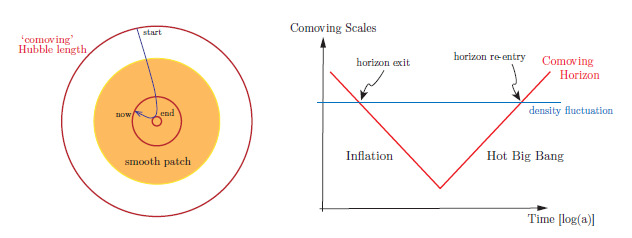
\includegraphics[width=0.7\textwidth]{horizon.png}
    \caption{\emph{Left}: Development of the inflationary universe's $(aH)^{-1}$ comoving Hubble radius. Inflation causes the co-moving Hubble sphere to contract and then expand. Hence, inflation serves as a tool to "zoom in" on a smooth sub-horizon patch. \emph{Right}: Solution of the horizon problem. All scales that are relevant to cosmological observations today were larger than the Hubble radius until $a \sim 10^{-5}$. These scales were, however, smaller than the Hubble radius at sufficiently early eras and were consequently causally related. Similarly, the scales of cosmological interest came back within the Hubble radius in relatively recent times.\cite{baumann2012tasi}}
    \label{fig:2.1} 
\end{figure}

\section{The Flatness Problem}
We saw in  section \ref{section 1.4} that the current measurements of the density parameters are compatible with a flat universe $\Omega_{total} \simeq 1 $.But the question arises how does $\Omega $ evolve with time?
We can write the Friedmann equation \ref{eq:1.43} as 
\begin{align}
    \Omega(t)-1 = \frac{k}{H(t)^{2} a(t)^{2}} \propto  \frac{k}{a^{2-3(1+w)}} = ka^{3w+1} \label{2.2}
\end{align}
We observe that for both radiation ($w = 1/3$) and matter ($w = 0$), we see that if $\Omega - 1 \neq 0$ at a certain early time then it will grow as $a^2$ or 
$a^4$ respectively and then the geometry of the present Universe is expected to be curved. So the near-flatness, we observe today requires the value of $\Omega(t)$ to be one. \\
By manipulating the Friedmann equation \ref{eq:1.43} we find

\begin{align}
  \Omega ^{-1} (z) -1
  = (\Omega_0 ^{-1} -1)\qty(\frac{T_0 }{T(z)})^{2} \,.
\end{align}

Let us extend this to the Planck epoch because the density at a time $t_P \approx 10^{-43}s$ must have been very close to the critical density. The temperature at that time was $T_P = \num{e32} K $. $T_{0}$ is the temperature today.


If we compute \(T _{\text{Pl}} / T_0 \) we get approximately \num{e32}.

This means that 
\begin{align}
    \Omega^{-1}(z_{\text{Pl}}) - 1 \approx (\Omega_0^{-1} - 1) \num{e-64}\,.
\end{align}
.As a result, the Universe should have needed to be extraordinarily finely tuned in order to imitate the flatness we observe today.

Using the Hubble radius, we can write to examine how the inflationary phase responds to this issue.
\begin{align}
    \Omega(t)-1 = \frac{k}{H(t)^{2} a(t)^{2}} = kr_{H}^2
\end{align}
In standard cosmology, the comoving Hubble radius grows with time,
therefore one expects the quantity $|\Omega(t)-1|$ to grow with time and the geometry of the present Universe to be curved. But,
if the universe undergoes a phase where the Hubble radius shrinks, this would bring $\Omega(t)$ closer to 1. It can be shown that the universe must expand by 60 e-foldings to achieve the flatness we observe today, as in the case of the horizon problem.



\section{Dynamics of Inflation}

\hspace{0.5cm}In the previous section, we saw that for inflation to take place we need  a phase of accelerated expansion ($\ddot{a} > 0$) where the Hubble radius($r_{H}$) shrinks.\\
We can see from the Friedmann Eq. \ref{eq:1.21a} that for an accelerated expansion
\begin{align}
    \ddot{a} = -\frac{4 \pi G}{3}(\rho+3P) > 0 \Rightarrow P < \frac{-\rho}{3}\,\label{2.6}
\end{align}
which we previously encountered in the  de-Sitter model where we found $a(t) \propto exp(\sqrt{\frac{\Lambda}{3}}t)$ and the expansion is driven by cosmological constant $\Lambda$, so we can have a calculated guess that the inflation can't be driven by matter or radiation. In the current  interpretation, $\Lambda$ is linked to the quantum fluctuations of the vacuum. The  vacuum expectation value of the stress-energy tensor gives the energy generated by these fluctuations.Using Eq. \ref{eq:1.19} and Eq. \ref{1.32} we can write
\\
\begin{align}
    \langle T_{\mu\nu} \rangle = -\langle P_{\Lambda} \rangle g_{\mu\nu} = \frac{\Lambda}{8\pi G} g_{\mu\nu} \label{2.7}
\end{align}
As a result, in this instance, the stress-energy tensor's vacuum expectation value functions as the cosmological constant that promotes the expansion. This provides an indication of what to anticipate from a theory describing the inflationary mechanism.

\subsection{Scalar(Inflaton) Field }





\hspace{0.5cm}To satisfy Eq. \ref{2.6} let us introduce a minimally coupled(i.e not coupled with gravity or any other field ) scalar field \(\varphi\)  with a suitable potential $V(\varphi)$ which is a self-interaction of the field. We can write its Lagrangian as 
\begin{align}
    \mathscr{L}_{\varphi} = -\frac{1}{2} g^{\mu\nu} \partial_{\mu}\varphi\partial_{\nu}\varphi - V(\varphi)\, \label{2.8}
\end{align}
The action is in the form of 

\begin{align}
    S = S_{EH} + S_\varphi + S _{\text{matter}}\,\label{2.9}
\end{align}

where \(S_{EH}\) is the Einstein-Hilbert action for the metric, \(S_\varphi \) is the action for the field \(\varphi \), while ``matter'' encompasses all the other fields but we can ignore it thanks to the \emph{no-hair cosmic theorem}.

\begin{align}
    S = \frac{1}{16 \pi G} \int \dd[4]{x} \sqrt{-g} R + \int \dd[4]{x} \sqrt{g} \mathscr{L}\varphi [\varphi , g{\mu \nu }],. \label{2.10}
\end{align}

We are using the invariant volume element \(\dd[4]{x} \sqrt{-g}\)
representing the physical 4-volume regardless of the coordinates.
Now, we can find the equation of motion for the inflaton field by  the Klein-Gordon equation by varying the action with respect to $\varphi$.
\begin{align}
    \square \varphi = \pdv{V}{\varphi }\,. \label{2.11}
\end{align}
where $\square$ is the covariant D'Alembert operator.
\begin{align}
    \square \varphi = \frac{1}{\sqrt{-g}} \qty(g^{\mu \nu } \sqrt{g} \varphi_{, \mu })_{, \nu }\,.\label{2.12}
\end{align}
and in a flat FRW metric Eq. \ref{eq:1.1} $\sqrt{-g} = a^3$ the evolution of $\varphi$ becomes
\begin{align}
    \square \varphi = \frac{1}{a^3} \partial_0 (g^{00} a^3\partial_0\varphi) + \frac{1}{a^3} \partial_i (g^{ii} a^3\partial_i\varphi) 
    &= \partial _{\varphi} V  \\ - \ddot{\varphi} - \dot{\varphi} 3\frac{\dot{a}}{a} + \frac{\nabla^2}{a^2} \varphi  
    &= \partial _{\varphi} V  \\ \ddot{\varphi} + 3 H \dot{\varphi} - \frac{\nabla^2 \varphi }{a^2} &= - \partial _{\varphi} V\,. \label{2.15}
\end{align}
where $3H\ddot{\varphi}$ appears as a friction term that is represented as a scalar field rolling down its potential suffering friction due to the expansion of the universe. If we consider the homogeneous background field, it will be constant in space, so  the above equation evolves as\\
\begin{align}
     \ddot{\varphi} + 3 H \dot{\varphi}  &= - \partial _{\varphi} V\,. \label{2.16}
\end{align}
The stress-energy tensor associated with the scalar field can be defined by 

\begin{align}
    T_{\mu \nu }^{(\varphi )} = - \frac{2}{\sqrt{-g}} \fdv{S_{\varphi }}{g^{\mu \nu }} =- 2 \frac{\partial\mathscr{L}_\varphi }{\partial g^{\mu \nu }} + \frac{2}{\sqrt{-g}} \mathscr{L}_\varphi \pdv{\sqrt{-g}}{g^{\mu \nu }} = - 2 \pdv{\mathscr{L}_\varphi }{g^{\mu \nu }} + \mathscr{L}_\varphi g_{\mu \nu }\\ = \partial_{\mu } \varphi \partial_{\nu } \varphi + g_{\mu \nu } \qty[- \frac{1}{2} g^{\alpha \beta } \partial_{\alpha } \varphi \partial_{\beta} \varphi - V(\varphi )] \,. \label{2.18}
\end{align}
If we compare it with Eq. \ref{eq:1.19} we find that $\varphi(t)$ behaves like a perfect fluid with
\begin{align}
    P &= -\frac{1}{2} g^{\alpha \beta }\partial_{\alpha } \varphi \partial_{\beta} \varphi - V(\varphi ) \label{2.19} \\
    \rho &= - \frac{1}{2} g^{\alpha \beta }\partial_{\alpha } \varphi \partial_{\beta} \varphi  + V(\varphi )  \label{2.20} \\
    u_\mu &= \frac{\partial_{\mu}\varphi}{\abs{\partial \varphi }}  \\
    \abs{\partial \varphi} &= \sqrt{- g^{\alpha \beta }\partial_{\alpha } \varphi \partial_{\beta} \varphi}
    \,.
\end{align}
\hspace{0.5cm}We start by considering $\varphi(t,x)$ and split it as
\begin{align}
    \varphi (\mathbf{x}, t) = \varphi(t) + \delta \varphi (\mathbf{x}, t) \, \label{2.23}
\end{align}
where $\varphi(t)$ is the classical field that is the expectation value of the inflaton field(\(\langle \varphi(t,x) \rangle = \varphi(t)\)) and $\delta \varphi(\mathbf{x}, t)\ $ represents the quantum fluctuations around $\varphi(t)$.
Now , 
\begin{align}
    \left|\frac{\delta \varphi(\mathbf{x}, t)}{\varphi(t)} \right| \ll 1 \label{2.24}
\end{align}
as quantum fluctuation is negligible in comparison to the classical value. These fluctuations are what generated the density fluctuation which creates anisotropies in the CMB photons. Let us drop the $"t"$ and indicate the value of the classic inflaton field by $\varphi$. On explicitly computing the energy-momentum tensor of the classical background $\varphi$ we find,
\begin{align}
    T^{0}_{0} &= - \qty( \frac{1}{2} \dot{\varphi}(t)^2 + V(\varphi )) = - \rho_\varphi\label{2.25}\\
    T^{i}_{j} &= \qty( \frac{1}{2} \dot{\varphi}^2 (t) - V(\varphi)) \delta^{i}_{j} = P_\varphi \delta^{i}_{j}\,. \label{2.26}
\end{align}
This is the perfect fluid energy-momentum tensor. Therefore, if 
\begin{align}
    V(\varphi) \gg \dot{\varphi}^2 ,\ \label{2.27}
\end{align}
we get $P_{\varphi} \simeq -\rho_{\varphi} \implies w_{\varphi} \simeq -1 $ i.e the quasi-de Sitter expansion.\\
So, we see that if the potential energy is greater than the kinetic energy  this scalar field gives inflation. For better intuition let us simplify the system and assume the vacuum expectation value of the inflaton to be constant i.e \(\langle \varphi(t,x) \rangle = \Bar{\varphi}\) then the stress-energy tensor becomes
\begin{align}
    \langle T_{\mu\nu} \rangle  = -g_{\mu\nu} V(\varphi) ,\ \label{2.28}
\end{align}
Comparing it to Eq. \ref{2.7} we see that the potential of the inflaton field $V(\varphi)$  represents the vacuum energy associated with $\varphi$ which drives the acceleration.\\

\subsection{Slow Roll Conditions}
\begin{figure}[h]
    \centering
    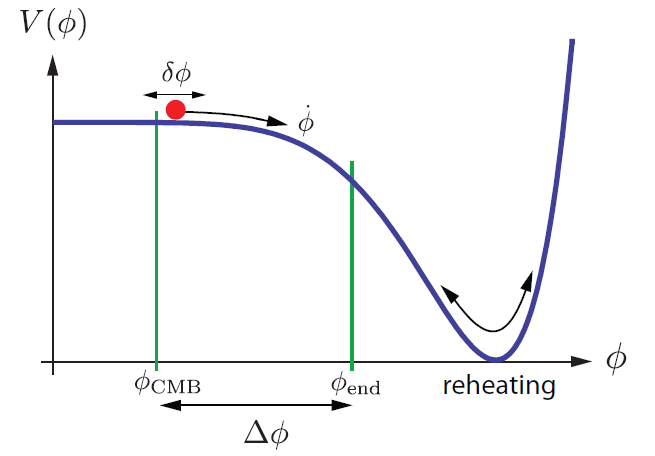
\includegraphics[width=0.7\textwidth]{inflaton.png}
    \caption{A possible shape of the potential for Slow-Roll Inflation \cite{baumann2012tasi}}
    \label{fig:2.2} 
\end{figure}
\hspace{0.5cm} Let us try to understand under what conditions the scalar field may initiate inflation. The equation of motion for the homogeneous scalar field is given in Eq. \ref{2.16}. To satisfy the condition given in Eq. \ref{2.27} the scalar field should slowly roll down its potential. The easiest way to satisfy the slow roll condition is to require that there exist regions of field-configuration space where the potential is sufficiently flat. Considering the potential to be flat the acceleration of the field should be negligible i.e
\begin{align}
    \ddot{\varphi} \ll 3H\dot{\varphi} \label{2.29}
\end{align}
We can also say as at a sufficiently late time the scalar field is driven by friction term. Therefore,
\begin{align}
    3H\dot{\varphi} \approx -\partial_{\varphi} V \label{2.30}
\end{align}
We expect that $V$ and all of its derivatives change very slowly with $\varphi$.
This means that in this equation we have \(\partial_{\varphi} V \approx const\), as well as \(H \approx const\): this is the same equation that is obeyed by a particle under a constant force and friction: it will then reach the asymptotic ``{terminal velocity}'' and move with a constant \(\dot{\varphi}_0 \).\\ 

So, the slow-roll condition is,
\begin{align}
     \ddot{\varphi} \ll (3H\dot{\varphi}),(-\partial_{\varphi} V )\label{2.31}
\end{align}\\
Let us now combine it with the Friedmann equation  \ref{eq:1.43},
\begin{align}
    H^2 = \frac{8 \pi G}{3} \qty(\rho _\varphi + \rho _m + \rho _r) - \frac{k}{a^2}\,.
\end{align}

The matter and radiation densities scale like \(a^{-3}\) for \(\rho _m\), \(a^{-4}\) for \(\rho _r\); in this early phase the scalar field dominates the dynamics, so the equation will simplify to 

\begin{align} \label{2.33}
    H^2 \approx \frac{8 \pi G}{3} V(\varphi)\,.
\end{align}
so, for a slow roll case, the Hubble parameter is nearly a constant and the scale factor is given by $a(t) \propto exp(Ht)$.\\
\hspace{0.5cm} We saw the slow roll conditions which are necessary for successful inflation. Next, we will parameterize it.

\
\hspace{0.5cm} These are the parameters we need to quantify in order to determine how closely the potential matches our expectations. It is given by $\epsilon$ and $\eta$. Let us start with the first parameter.\\
We define $\epsilon$ as,
\begin{align}
    \epsilon = -\frac{\dot{H}}{H^2}. \label{2.34}
\end{align}
As we saw previously for inflation to take place the Hubble radius shrinks. So let us write this in terms of the $\epsilon$ parameter.
\begin{align}
    \dv{(aH)^{-1}}{t} = \frac{-\dot{a}H + a\dot{H}}{(aH)^2} = -\frac{1}{a}\left( 1- \left( \frac{-\dot{H}}{H^2}\right)\right) = -\frac{1}{a}(1 - \epsilon) \label{2.35}
\end{align}
so we see that if $\dot{r_H} < 0$ implies that $\epsilon \ll 1 $.\\
\hspace{0.5cm} Using Eq. \ref{2.30} and Eq. \ref{2.33} we can write $\epsilon$ as,
\begin{align}
    \epsilon = - \frac{\dot{H}}{H^2} = + 4 \pi G \frac{\dot{\varphi}^2}{H^2} \approx \frac{3}{2} \frac{\dot{\varphi}^2}{V} = \frac{1}{16 \pi G} \qty(\frac{\partial_{\varphi} V}{V})^2\,,\label{2.36}
\end{align}
so the condition $\epsilon \ll 1 $ can also be written as 
\begin{align}
    \frac{(\partial_{\varphi} V)^2}{16 \pi G V^2} &\ll 1  \\ 
    \frac{(\partial_{\varphi} V)^2}{V} &\ll 16 \pi G V = \frac{2}{3} H^2 \\ 
    \frac{1}{V} \qty(\pdv{V}{\varphi })^2 &\ll H^2\,.\label{2.39}
\end{align}
on using Eq. \ref{2.34} we can see that it is exactly the slow roll condition in Eq. \ref{2.27}, So, we see that $\epsilon$ gives a bound on the first derivative of the potential and corresponds to the conditions of the potential being flat and the kinetic energy being small compared to the potential.\\
The second derivative of the potential is controlled by the parameter $\eta$ which is defined as,
 \begin{align}
     \eta = - \frac{\ddot{\varphi}}{H \dot{\varphi}}\,, \label{2.40}
 \end{align}
 and we can also define 

\begin{align}
    \eta = \frac{1}{3} \frac{\partial^{2} _{\varphi} V}{H^2} = \frac{1}{8 \pi G} \frac{\partial^{2} _{\varphi} V}{V} \,. \label{2.41}
\end{align}

We can see that \(\eta \ll 1 \) is equivalent to
\begin{align}
    \pdv[2]{V}{\varphi} \ll H^2 \label{2.42}
\end{align}

We can show that these three parameters are related  \(\delta = \eta - \epsilon \).\\
We start from Eq. \ref{2.30} and differentiate it with respect to the time we get 

\begin{align}
    \ddot{\varphi} &\approx - \dv{}{t} \qty( \frac{\partial_{\varphi} V}{3H})  \\ &= - \frac{1}{3H} \partial^{2} _{\varphi} V \dot{\varphi} - \frac{\partial_{\varphi} V}{3} \underbracket{\qty(- \frac{\dot{H}}{H^2})}_{\epsilon }  \\ &= - \dot{\varphi} H \frac{\partial^{2} _{\varphi} V}{3H^2} - \frac{\partial_{\varphi} V}{3} \epsilon  \\ &= - \dot{\varphi} H \eta - \frac{\partial_{\varphi} V}{3} \epsilon  \\ {-\frac{\ddot{\varphi}}{H \ddot{\varphi}}} &= \eta - \epsilon  \\
    \delta &= \eta - \epsilon,.\label{2.48}
\end{align}
which is the desired result.
We see that $\delta \ll 1 $ corresponds to the condition $\ddot{\varphi} \ll -\partial_{\varphi} V$, which is required in order to neglect the acceleration term in the Klein-Gordon equation. So, the condition  $\delta \ll 1 $ ensures that we move towards an attractor solution in the friction-dominated regime i.e, it will then reach the asymptotic “terminal velocity” and move with a constant $\dot{\varphi}$. Also, for inflation to solve the horizon and the flatness problem  we need a phase of accelerating expansion that lasts sufficiently long. For this to happen, we need $\epsilon \sim const$, since $\epsilon \sim \dot{\varphi}$ while $\delta \sim \ddot{\varphi}$, so requiring $\delta \ll 1$ also ensures this.
.\\
\hspace{0.5cm}In summary, the slow-roll approximation described in Eq. \ref{2.27} and Eq. \ref{2.31} implies the inflationary potential's flatness under conditions Eq. \ref{2.36} and Eq. \ref{2.41}.\\



\section{Inflation-Induced Cosmological Perturbations} \label{section 2.4}
 Inflationary cosmology relies on understanding the evolution of quantum fluctuations of the inflaton field $\delta \varphi(\mathbf{x},t)$, which give rise to primordial energy density perturbations that persist after inflation and form the basis of the large-scale structures observed in the Universe. These fluctuations arise on extremely small scales within the comoving Hubble radius during inflation, but the rapid expansion of space during this epoch stretches them out to cosmological scales. As the Hubble radius begins to increase faster than the scale factor after inflation ends, these fluctuations eventually re-enter the Hubble radius during the radiation or matter-dominated eras. The fluctuations that re-enter around 60 e-foldings before reheating have physical wavelengths that can be observed through various methods, such as the analysis of CMB anisotropies. The resulting inflationary spectrum provides a unique and distinct signature of inflation that can help us understand the origins of structure in the Universe. \\

 \begin{figure}[h]
    \centering
    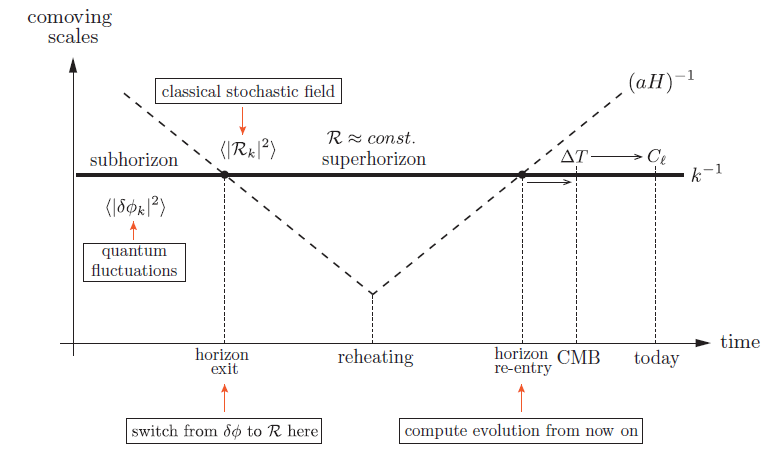
\includegraphics[width=0.7\textwidth]{comving vs conformal time.png}
    \caption{Creation and evolution of perturbations in the inflationary universe. On subhorizon scales, quantum mechanics produces fluctuations. During inflation, comoving scales, $k^{-1}$, stay constant in the comoving Hubble radius, but  $(aH)^-{1}$ diminishes and the perturbations leave the horizon, where they remain frozen until horizon re-entry at later times. The fluctuations change into anisotropies in the CMB and disturbances in the LSS after horizon re-entry. Taken from \cite{baumann2012tasi}}
    \label{fig:2.3} 
\end{figure}

\subsection{Dynamics of Quantum Fluctuations: Qualitative Analysis}

 \hspace{0.5cm} Let us now describe qualitatively how the quantum fluctuations of a generic scalar field evolve during an inflationary stage. We saw the dynamics of the scalar field obey the Klein-Gordon Eq. \ref{2.15} which we Taylor expand upto linear order around the background value for both $\varphi$ Eq. \ref{2.23} and for the potential \(V(\varphi ) \approx V_0 + \delta \varphi \eval{(\pdv{V}{\varphi })}_{\varphi_0 }\). Assuming the perturbation is indeed small we can write the Klein-Gordon equation for the fluctuation as

\begin{align} 
    \ddot{ \delta \varphi} + 3 H \dot{\delta \varphi} - \frac{\nabla^2}{a^2} \delta \varphi = - \pdv[2]{V(\varphi )}{\varphi } \delta \varphi \,. \label{2.49}
\end{align}
Let us move to the Fourier space which is more convenient for the problem. We can write,
\begin{align}
    \delta \varphi (\mathbf{x}, t) = \frac{1}{(2\pi )^{3}} \int \dd[3]{k} 
    e^{i \mathbf{k} \cdot \mathbf{x}} \delta \varphi _{\mathbf{k}}(t)
    \,.\label{2.50}
\end{align}
Since the field is real, \(\delta \varphi _{\mathbf{k}} = \delta \varphi _{- \mathbf{k}}^{*}\).\\
Now we will write the Klein-Gordon equation  for the quantum fluctuation in Fourier space.

\begin{align}
    \ddot{ \delta \varphi} _{\mathbf{k}} + 3 H \dot{ \delta \varphi}_{\mathbf{k}} + \frac{k^2}{a^2} \delta \varphi _{\mathbf{k}} = - \partial_{\varphi}^2(V) \delta \varphi _{\mathbf{k}}\,.\label{2.51}
\end{align}

If we consider a massless scalar field $\partial_{\varphi}^2(V) \approx 0$ which corresponds to the requirement of the parameter $\eta \ll 1$ which we discussed in the previous section. So, we can write the above equation as

\begin{align}
    \ddot{ \delta \varphi} _{\mathbf{k}} + 3 H \dot{ \delta \varphi}_{\mathbf{k}} + \frac{k^2}{a^2} \delta \varphi _{\mathbf{k}} \simeq 0 \label{2.52}
\end{align}\\

Now let us distinguish between the \textbf{sub-horizon}($\lambda < r_H$) and the \textbf{super-horizon}($\lambda > r_H$) regimes on the basis of the comoving wavelength $\lambda_{com} a(t) = \lambda_{physical} \simeq 2\pi/k_{physical}$

\begin{itemize}
    \item  \textbf{sub-horizon}($\lambda < r_H$):\\
    \begin{equation}
        \lambda \ll \frac{1}{aH} \implies \frac{k}{aH} \gg 1\ \label{2.53}
    \end{equation}
    We can write Eq. \ref{2.52} as
    \begin{align}
        \ddot{ \delta \varphi} _{\mathbf{k}} + (3 H^2  + \frac{k^2}{a^2}) \delta \varphi _{\mathbf{k}} &=  \ddot{ \delta \varphi} _{\mathbf{k}} + \frac{k^2}{a^2} \delta \varphi _{\mathbf{k}} \simeq 0 \label{2.54}
    \end{align}  
    
    where we used the Hubble time scale \(t_{\mathrm{H}}=H^{-1}\) as the time reference and the sub-horizon condition Eq. \ref{2.53}. So we observe that in the sub-horizon regime, the Fourier transform of the quantum fluctuations of the scalar field $\delta \varphi_{\mathbf{k}}$ can be described by a harmonic oscillator equation with a  frequency term given by the factor $k / a(t)$ where the scale factor depends upon time as  \(a(t) \propto e^{Ht}\). This behaviour is expected, as at small scales inside the horizon, the local space-time appears flat like Minkowski space-time, and the expansion of the universe is negligible.
    
     \item  \textbf{super-horizon}($\lambda > r_H$):\\
    \begin{equation}
        \lambda \gg \frac{1}{aH} \implies \frac{k}{aH} \ll 1, \label{2.55}
    \end{equation}
    In this regime, we proceed as in the sub-horizon regime and observe that for the above condition given in Eq. \ref{2.55}
    \begin{align}
       3 H^{2} \delta \varphi_{\mathbf{k}} \ll \frac{1}{a^{2}} k^{2} \delta \varphi_{\mathbf{k}} \label{2.56}
    \end{align}
    which shows that the friction term is dominant with respect to the Laplacian, therefore we can write Eq.\ref{2.52} as
    \begin{align}
        \ddot{ \varphi_{\mathbf{k}}}+3 H \dot{\delta} \varphi_{\mathbf{k}} \simeq 0 \label{2.57}
    \end{align}    
    The solution for the above second-order differential Eq. \ref{2.57} is given by
   \begin{align}
        \delta \varphi_{\mathbf{k}}=A+B e^{-3 H t} .
    \end{align}
    
    from this, we can interpret that as the exponential term decays and we get towards a constant fluctuation. In other words, as time increases the fluctuation oscillates until the wavelength gets larger than the Hubble horizon
    (maximum distance of causal connection), as soon as it is larger, the fluctuations cant interact nor grow and they cease to oscillate and get \emph{"frozen-in"}
\end{itemize}


\subsection{Dynamics of Quantum Fluctuations: exact solution}

In this section, we will discuss the exact solution to the dynamics of quantum fluctuation of a more generic scalar field \(\hat{\delta \varphi}(\tau, \mathbf{x}) \)  that includes quantum field theory effects and the mass term given by $\partial_{\varphi}^{2} V$. As done in the previous section, we explore the solution in the sub-horizon and super-horizon limits.

We start by redefining the field as,
\begin{align}
    \hat{\delta \varphi}(\tau, \mathbf{x})=a(\tau) \delta \varphi(\tau, \mathbf{x}) ,\
\end{align}

here we need to take into note that we are using conformal time $\tau$  instead of cosmic time. Now, we can write the generic scalar field  $\hat{\delta \varphi}(\tau, \mathbf{x})$ as a linear combination of the creation-annihilation operators $\left(a_{\mathbf{k}}, a_{\mathbf{k}}^{\dagger}\right)$

\begin{align}
    \hat{\delta \varphi}(\tau, \mathbf{x})=\frac{1}{(2 \pi)^{3}} \int \mathrm{d}^{3} \mathrm{k}\left[u_{\mathbf{k}}(\tau) a_{\mathbf{k}} e^{i \mathbf{k} \cdot \mathbf{x}}+u_{\mathbf{k}}^{*}(\tau) a_{\mathbf{k}}^{\dagger} e^{-i \mathbf{k} \cdot \mathbf{x}}\right]
\end{align}

and time-dependent mode functions $u_{\mathbf{k}}(\tau)$ that obeys a normalization condition
% In quantum field theory, a mode function describes the behaviour of a quantum field in terms of its wave-like properties. The normalization condition for a time-dependent mode function can be obtained by requiring that the total number of particles associated with the field is conserved.

\begin{align}
    u_{\mathbf{k}}^{\prime *}(\tau) u_{\mathbf{k}}(\tau)-u_{\mathbf{k}}^{*}(\tau) u_{\mathbf{k}}^{\prime}(\tau)= -i
\end{align}

such that commutation rules are given by


\begin{align}
    & {\left[a_{\mathbf{k}}, a_{\mathbf{k}^{\prime}}\right]=\left[a_{\mathbf{k}}^{\dagger}, a_{\mathbf{k}^{\prime}}^{\dagger}\right]=0,} \\
    & {\left[a_{\mathbf{k}}, a_{\mathbf{k}^{\prime}}^{\dagger}\right]=\hbar \delta^{(3)}\left(\mathbf{k}-\mathbf{k}^{\prime}\right) .}
\end{align}

In the Minkowski space-time the solutions i.e the mode functions are described by plane waves such as

\begin{align}
   u_{\mathbf{k}}(\tau) \sim \frac{e^{-i \omega_{\mathbf{k}} \tau}}{\sqrt{2 \omega_{\mathbf{k}}}}, \quad \omega_{\mathbf{k}}=\sqrt{k^{2}+m^{2}} .
 \end{align}


However, in the case of an expanding FRW Universe, we have a curved space-time, and we expect a more complicated expression for $u_{\mathbf{k}}(\tau)$. Since, in quantum field theory on curved space-time, the choice of the vacuum state is not unique enough to determine the mode functions due to the presence of the gravitational field. This means that different choices of vacuum state can result in different sets of mode functions, which can affect the physical properties of the theory. So, in short in quantum field theory on curved space-time there is an ambiguity with the choice of the vacuum state, therefore $u_{\mathbf{k}}(\tau)$ is not a priori fixed.\\
Looking at the equivalence principle as a guiding principle, modes \(u_{k} (\tau)\) at very short distances must reproduce the form for the ordinary flat space-time quantum field theory, which is the plane waves. So, we require  \begin{align}
    \frac{k}{aH} \rightarrow \infty \implies \  u_{\mathbf{k}}(\tau) \sim \frac{e^{-i \mathbf{k} \tau}}{\sqrt{2\mathbf{k}}}, \quad \sqrt{k^{2}+m^{2}} \simeq k  \label{2.65}   
\end{align}which is the Bunch-Davies condition on the vacuum state, which states that in the limit of small scales and for initial times the mode functions are given by
\begin{align}
    u_{\mathbf{k}}(\tau) \rightarrow \frac{e^{-i \mathbf{k} \tau}} {\sqrt{2\mathbf{k}}}. \label{2.66}
\end{align}
To motivate the inflationary vacuum state we try to recall our previous discussion that at a sufficiently early time all the modes of cosmological interest were deep inside the horizon i.e, which implies $k/aH \gg 1$ so, we can write $w_{k} \simeq k$ and there the mode function is given by Eq. \ref{2.66}\\
\hspace{0.5cm} Before rewriting equation 2.45 in the Fourier space, we will explicitly change the time coordinate going from the reference time $t$ to the conformal time $\tau$ such that

\begin{align}
    \frac{d}{d t} \quad \longrightarrow \quad \frac{d}{d t} \frac{d \tau}{d \tau}=\frac{1}{a} \frac{d}{d \tau} \label{2.67}
\end{align}

let us  perform the calculations term by term using the coordinate change in equation \ref{2.67}. On the left-hand side of equation \ref{2.51} we have


\begin{align}
    \delta \ddot{\varphi}_{\mathbf{k}} & =\frac{1}{a} \frac{d}{d \tau}\left[\frac{1}{a} \frac{d}{d \tau}\left(\frac{\delta \hat{\varphi}_{\mathbf{k}}}{a}\right)\right] \\
    & =\frac{1}{a} \frac{d}{d \tau}\left[\frac{1}{a}\left(\frac{\delta \hat{\varphi}_{\mathbf{k}}^{\prime}}{a}-\frac{a^{\prime}}{a^{2}} \delta \hat{\varphi}_{\mathbf{k}}\right)\right] \\
    & =\frac{1}{a}\left(\frac{\delta \hat{\varphi}_{\mathbf{k}}^{\prime \prime}}{a^{2}}-2 \frac{a^{\prime}}{a^{3}} \delta \hat{\varphi}_{\mathbf{k}}^{\prime}-\frac{a^{\prime \prime}}{a^{3}} \delta \hat{\varphi}_{\mathbf{k}}-3 \frac{a^{\prime 2}}{a^{4}} \delta \hat{\varphi}_{\mathbf{k}}-\frac{a^{\prime}}{a^{3}} \delta \hat{\varphi}_{\mathbf{k}}^{\prime}\right) \\
    & =\frac{\delta \hat{\varphi}_{\mathbf{k}}^{\prime \prime}}{a^{3}}-2 \frac{a^{\prime}}{a^{4}} \delta \hat{\varphi}_{\mathbf{k}}^{\prime}-\frac{a^{\prime \prime}}{a^{4}} \delta \hat{\varphi}_{\mathbf{k}}+3 \frac{a^{\prime 2}}{a^{5}} \delta \hat{\varphi}_{\mathbf{k}}-\frac{a^{\prime}}{a^{4}} \delta \hat{\varphi}_{\mathbf{k}}^{\prime},
\end{align}


and


\begin{align}
    3 H \delta \dot{\varphi}_{\mathbf{k}} & =3 \frac{1}{a^{2}} \frac{d a}{d \tau} \frac{1}{a} \frac{d}{d \tau}\left(\frac{\delta \hat{\varphi}_{\mathbf{k}}}{a}\right) \\
    & =3 \frac{a^{\prime}}{a^{4}} \delta \hat{\varphi}_{\mathbf{k}}^{\prime}-3 \frac{a^{\prime 2}}{a^{5}} \delta \hat{\varphi}_{\mathbf{k}}
\end{align}


Finally, putting all the results together, we obtain

\begin{align}
    \delta \hat{\varphi}_{\mathbf{k}}^{\prime \prime}-\frac{a^{\prime \prime}}{a} \delta \hat{\varphi}_{\mathbf{k}}+k^{2} \delta \hat{\varphi}_{\mathbf{k}}=-\partial_{\varphi}^{2} V a^{2} \delta \hat{\varphi}_{\mathbf{k}} \label{2.74}
\end{align}

which in terms of the mode functions can be written as

\begin{align}
    u_{\mathbf{k}}^{\prime \prime}(\tau)+\left(k^{2}-\frac{a^{\prime \prime}}{a}+\partial_{\varphi}^{2} V a^{2}\right) u_{\mathbf{k}}(\tau)=0 . \label{2.75}
\end{align}

 From this, we can see why we chose to use the re-scaled version  $\delta \hat{\varphi}_{\mathbf{k}}$. We can notice that the \emph{ansatz} is basically a harmonic oscillator with a time-dependent frequency changing according to the accelerated expansion of the universe. Let us look at the behavior of the mode function in the sub-horizon and super-horizon regimes for a de Sitter Universe and a quasi-de Sitter Universe.

\subsection*{Solution in de-Sitter}
To solve the equation we will first consider the de-Sitter expansion where $H = constant$, $\epsilon \rightarrow 0$  and we assume the inflation is massless i.e 
\(m_{\varphi}^2 = \partial_{\varphi}^2{V} = 0\)
Under these conditions, we can write the  conformal time given by \ref{eq:1.8} as

\begin{align}
    d \tau=\frac{d t}{a(t)}=d t e^{-H t} \label{2.76}
\end{align}

where we used the $a(t) \propto e^{Ht}$. After integration, we obtain the corresponding scale factor which reads as

\begin{align}
    a(\tau) = -\frac{1}{H\tau}(\tau < 0)  \label{2.77}
\end{align}
and
\begin{align}
    \frac{a''}{a} = 2a^2H^2 \label{2.78}
\end{align}

which on plugging it into Eq. \ref{2.75} gives

\begin{align}
    u_{\mathbf{k}}^{\prime \prime}(\tau)+\left(k^{2}-2 a^{2} H^{2}\right) u_{\mathbf{k}}(\tau)=0 .\label{2.79}
\end{align}



In the \textbf{sub-horizon}($k \gg a H$) limit, Eq. \ref{2.79} becomes

\begin{align}
    u_{\mathbf{k}}^{\prime \prime}(\tau)+k^{2} u_{\mathbf{k}}(\tau)=0 \quad \Rightarrow \quad u_{\mathbf{k}}(\tau)=\frac{e^{-i k \tau}}{\sqrt{2 k}} \label{2.80}
\end{align}


where we chose the Bunch-Davies vacuum state. As predicted in the qualitative analysis in the previous section, the behavior of quantum fluctuations with wavelength within the cosmological horizon oscillates as we saw before in a flat space-time quantum field theory. This is what was expected for wavelengths much smaller than the Hubble radius scale where it is a good approximation to approximate the space-time as flat.\\

In the \textbf{super-horizon regime} ($k \ll aH$), Eq. \ref{2.79} approximates as

\begin{align}
    u_{\mathbf{k}}^{\prime \prime}(\tau)-\frac{a^{\prime \prime}}{a} u_{\mathbf{k}}(\tau)=0 \label{2.81}
\end{align}



whose solution is simply given by

\begin{align}
    u_{\mathbf{k}}(\tau)=\underbracket{B(k) a(\tau)}_{\text{growing mode}}+ \underbracket{C(k) a(\tau)^{-2}}_{\text{decaying mode}} .\label{2.82}
\end{align}

 We see that  the solution has a growing and a decaying mode where the decaying mode decays in time as $a(\tau)^{-2}$, so we can neglect the decaying mode because even if the amplitude increases it will decay quickly. Therefore the amplitude of the physical fluctuation reads as

\begin{align}
    \left|\delta \varphi_{\mathbf{k}}\right| \propto \frac{\left|u_{\mathbf{k}}\right|}{a(\tau)}=|B(k)| \label{2.83}
\end{align}

In the above equation, we can see that the “growing
mode” is actually asymptotically constant on super-horizon scales since $|B(k)|$ is independent of $\tau$.
To determine the scale of $B(k)$ we need to match the super-horizon and sub-horizon solutions, so it is basically a link between the quantum perturbation at horizon exit time during inflation and perturbation at horizon re-entry time during radiation or matter-dominated era. We thus evaluate $|B(k)|$ at the time of horizon crossing during inflation and we get

\begin{align}
    \abs{B(k)} a &= \abs{\frac{e^{-ik \tau }}{\sqrt{2 k}}} \label{2.84}  \\
    \abs{ \delta \varphi _\textbf{k}} &= \abs{B(k)} = \frac{1}{a \sqrt{2k}} 
    = \frac{H}{\sqrt{2 k^3}}\label{2.85}
    \,.
\end{align}

The fluctuation gets ``frozen in'' at horizon crossing: 

\begin{align}
    \abs{ \delta \varphi _\textbf{k}} = \frac{H}{\sqrt{2 k^3}}
    \,.
\end{align}

 Without proof, we will state the following result: the exact solution for the perturbation growth in De Sitter space-time is 

\begin{align}
     u_{\mathbf{k}}(\tau ) &= \frac{e^{ik \tau }}{\sqrt{2 k}} \qty(1 - \frac{i}{k \tau })
    \,.
\end{align}

As shown above, the physics underlying small scales below the horizon is described by special relativity, while quantum fluctuations around the vacuum expectation value of the scalar field are treated using quantum field theory in flat space-time. These fluctuations have a mean value of zero due to the nature of the vacuum state, which is characterized by the creation and annihilation of particles with a net number of particles equal to zero.

During inflation, the comoving Hubble radius shrinks, causing the rapid expansion to stretch the wavelength of the quantum fluctuations. This results in all fluctuations generated at sub-horizon scales exiting the horizon, where their amplitudes become frozen and are not affected by causal contact. After inflation ends, the comoving horizon begins to grow again, causing all fluctuations to re-enter the horizon with an imprint of their primordial fluctuations generated by inflation but with a much larger physical wavelength.

\subsection*{Solution in Quasi- de Sitter}
In this section, we will see how to solve the equation \ref{2.74} explicitly 

\begin{align}
    u''_{\mathbf{k}} (\tau )
    + 
    \qty[k^2 - \frac{a''}{a} + a^2 m^2]  u_{\mathbf{k}}(\tau ) = 0\label{2.88}
    \,,
\end{align}

where \(\tau \) is the conformal time, while \(m^2 = \pdv*[2]{V}{\varphi }\). 
The stage in which \(m^2 = 0\) is the quasi-de-Sitter stage. 
Now we will consider that \(H\) is not a constant, instead, we will consider the effect of a nonzero slow-roll parameter \(\epsilon = - \dot{H} / H^2 \ll 1\). 
.We will use the relation
\begin{align}
    \frac{\ddot{a}}{a} = H^2 ( 1- \epsilon ) \label{2.89}
    \,,
\end{align}
which can be proven by straightforward manipulation.\\

Using the definition of the conformal time, we can show that the scale factor for small values of $\epsilon$ becomes

\begin{align}
    \tau = - \frac{1}{a H (1 - \epsilon )}\label{2.90}
\end{align}
\
 
Using this, we find that to first order 
\begin{align}
    (aH)^2 \approx (1 + 2 \epsilon ) / \tau^2 \label{2.91}
\end{align}
therefore we can re-write eq \ref{2.89}  using eq \ref{2.91} in terms of conformal time as,

\begin{align}
    \frac{a''}{a} = a^2 H^2 (2- \epsilon ) 
    =2 \frac{(1 + 2 \epsilon)}{\tau^2} \qty(1 - \frac{\epsilon}{2})
    \approx \frac{2}{\tau^2} \qty(1 + \frac{3}{2} \epsilon ) \label{2.92}
    \,.
\end{align}

Substituting this for \(a'' /a\) the equation becomes 

\begin{align}
    u''_{\mathbf{k}}(\tau ) + \qty[k^2 - \frac{\nu^2 - 1/4}{\tau^2}]  u_{\mathbf{k}}(\tau )= 0 \,,\label{2.93}
\end{align}

where \(\nu^2 = 9/4 + 3 \epsilon \). 
This is a Bessel equation: these equations are generally in the form 

\begin{align}
    z^2 y'' (z) + z y' (z) + (z^2 - \nu^2) y(z) = 0\,.
\end{align}

The solutions are called Hankel functions, assuming \(\nu\) as constant the general solution is given as

\begin{align}
     u_{\mathbf{k}}(\tau ) = \sqrt{- \tau } \qty[ c_1 (k) H_\nu^{(1)} (-k\tau ) + c_2 (k) H_\nu^{(2)} (-k\tau )] \,\label{2.95}
\end{align}

where \(H^{(2)}_\nu = H^{(1)*}_\nu\). 
We want to impose the asymptotic behavior of the solution: let us start with 
\begin{itemize}
    \item \textbf{Sub-horizon (\(k / aH \gg 1\)):}\\ . 
    This means that 
    
    \begin{align*}
         u_{\mathbf{k}}(\tau ) = \frac{1}{\sqrt{2k}} e^{-ik \tau }
        \,,
    \end{align*}
        
    
    
    and the asymptotics of the Hankel functions are
    
    \begin{align}
        H^{(1)}_\nu  (x) \sim \sqrt{ \frac{2}{\pi x}} \exp(i \qty(x - \frac{\pi}{2} \nu - \frac{\pi}{4})) \sim \frac{e^{ix}}{\sqrt{x}} \, \label{2.96}
    \end{align}
    
    for \(x \gg 1\). This works well for us: we can set \(c_2 (k) = 0\) and only use \(c_1 (k)\). 
    
    We must choose 
    
    \begin{align}
        c_1 (k) = \frac{\sqrt{\pi }}{2} \exp(i \qty(\nu + \frac{1}{2}) \frac{\pi}{2})\,\label{2.97}
    \end{align}
    
    in order to have the correct normalization. 
    Then, our solution will read 
    
    \begin{align}
         u_{\mathbf{k}}(\tau ) = \frac{\sqrt{\pi }}{2} \exp(i ( \nu + \frac{1}{2}) \frac{\pi}{2}) \sqrt{-\tau } H^{(1)}_\nu (- k \tau )
        \,,\label{2.98}
    \end{align}
    \item \textbf{Super-horizon (\(k /aH \ll 1\)):}\\
    We have the asymptotic \(x \ll 1\) expansion of the Hankel function:

    \begin{align}
        H^{(1)}_\nu (x) \sim \sqrt{ \frac{2}{\pi }} e^{- i \pi /2}
        2^{\nu - 3/2} \frac{\Gamma (\nu )}{\Gamma (3/2)} x^{-\nu } \sim x^{-\nu }
        \,,\label{2.99}
    \end{align}
    
    therefore 
    
    \begin{align}
         u_{\mathbf{k}}(\tau ) \approx \exp(i (\nu - \frac{1}{2}) \frac{\pi}{2})
        2^{\nu - 3/2}
        \frac{\Gamma (\nu )}{\Gamma (3/2)}
        (- k \tau )^{1/2 - \nu } \frac{1}{\sqrt{2 k}} 
        \,,\label{2.100}
    \end{align}
\end{itemize}

so for getting the modulus \(\abs{ \delta \varphi _{\mathbf{k}}} = \abs{ u_{\mathbf{k}}} / a\) we can  use the fact that \(\tau \sim - 1/aH\), therefore \(\abs{ \delta \varphi _k} \approx - H \tau \abs{u_k}\). 
Inserting the expression we have for \(u_k\) we get,

\begin{align}
    \abs{ \delta \varphi _{\mathbf{k}}} 
    &\approx 2^{\nu - 3/2} \frac{\Gamma (\nu )}{\Gamma (3/2)} \frac{H}{\sqrt{2 k^3}} \qty(\frac{k}{aH})^{3/2 - \nu } \label{2.101} \\
    &\approx \frac{H}{\sqrt{2 k^3}} \qty( \frac{k}{aH})^{3/2 - \nu }
    \approx \frac{H}{\sqrt{2 k^3}} \qty( \frac{k}{aH})^{-\epsilon }
    \marginnote{Expanded to first order in \(\epsilon \), so that \(3/2 - \nu \approx - \epsilon \).}
    \,,\label{2.102}
\end{align}

which holds at super-horizon scales. In the De Sitter case, the exact result reads

\begin{align}
 u_{\mathbf{k}}(\tau ) \propto \sqrt{- \tau } H^{(1)}_{3/2} (- k \tau )
= \frac{e^{-ik \tau }}{\sqrt{2k}} \qty(1 - \frac{i}{k \tau })
\,.\label{2.103}
\end{align}\\

% The next step is to generalize to a scalar field that is not massless anymore: we shall consider a mass $m^2 = \frac{\partial^2 V}{\partial \varphi^2} \ll H^2$, so a "light" scalar field. We require this because one of the slow-roll parameters is $\eta_V = \frac{m^2}{3H^2} \ll 1$: a massive field (compared to $H^2$) would not be able to drive slow-roll inflation. 

% Then, the \(m^2 a^2\) term in the equation is nothing but 
% The next step is to generalize to a scalar field that is not massless anymore: we shall consider a mass $m^2 = \frac{\partial^2 V}{\partial \varphi^2} \ll H^2$, so a "light" scalar field. We require this because one of the slow-roll parameters is $\eta_V = \frac{m^2}{3H^2} \ll 1$: a massive field (compared to $H^2$) would not be able to drive slow-roll inflation.

% Then, the $m^2 a^2$ term in the equation is nothing but the mass term of the scalar field in an expanding universe. Since we are considering a "light" scalar field with a mass much smaller than the Hubble parameter, this term is much smaller than the $H^2$ term and can be neglected during inflation. This allows the scalar field to slowly roll down its potential, driving inflation. The slow-roll parameter $\eta_V$ is a measure of how much the scalar field's mass affects inflation, and a small value of $\eta_V$ is necessary for inflation to occur.
\hspace{0.5cm}Let's take a step forward in generalizing the scalar field with non-zero mass, denoted by $m^2 = \frac{\partial^2 V}{\partial \varphi^2}$. We require this mass to be much smaller than the Hubble parameter, $H$. This condition ensures that the scalar field can drive inflation through slow-roll. Specifically, we need the slow-roll parameter $\ \eta_V = \frac{m^2}{3H^2} \ll 1$.

The reason for this requirement is that a massive scalar field (compared to $H^2$) would not be able to maintain the slow-roll conditions needed for inflation. In other words, its mass would dominate over the Hubble friction term and prevent the scalar field from smoothly rolling down its potential.

 Then, the \(m^2 a^2\) term in the equation represents the mass term of the scalar field in an expanding universe which can be written as
\begin{align}
    m^2 a^2 = 3 \eta a^2 H^2 = \frac{3 \eta}{\tau^2}\label{2.104}
    \,,
\end{align}

but we also know that 

\begin{align}
    \frac{a''}{a} = \frac{2}{\tau^2 } \qty[ 1 + \frac{3}{2} \epsilon ]
    \,, \label{2.105}
\end{align}
%
Hence, the equation can still be recast into the same Bessel form but this time only the coefficient of the \(\tau^{-2}\) term changes.

The equation will read 
%
\begin{align}
    u''_{\mathbf{k}} (\tau ) + \qty[ k^2 - \frac{\nu^2 - 1/4}{\tau^2}]  u_{\mathbf{k}}(\tau ) = 0
    \,,\label{2.106}
\end{align}
%
with \(\nu^2 = 9/4 + 3 \epsilon - 3 \eta\). 
Then, the solution has exactly the same form as before:\\
on super-horizon scales, with \(k \ll aH\), we have
%
\begin{align}
    \abs{ \delta \varphi _k} = \frac{H}{\sqrt{2 k^3}} \qty( \frac{k}{aH})^{3/2 - \nu }
    &&
    \nu \approx \frac{3}{2} + \epsilon - \eta
    \,.\label{2.107}
\end{align}

It's worth noting that the previous computation doesn't only apply to an inflaton field, but also to any scalar field evolving during this phase of the universe's expansion. However, it's important to consider the field's mass - it can be shown that if $m^2$ is much greater than $H^2$, the super-horizon fluctuations of the field will have difficulty being excited and the field will remain in its vacuum state. So, if it's another scalar field, it needs to be light to be able to generate super-horizon fluctuations.








\section{The Power Spectrum} \label{section 2.5}
The power spectrum is a useful quantity to characterize the properties of a perturbation field which helps us to connect theoretical predictions with observational

The properties of a Gaussian random field $\delta(t, \mathbf{x})$ that represents a fluctuation in a point of space-time, such as the density fluctuation, can be described by an infinite set of correlation functions. These functions are defined as:

\begin{align}
    &\xi\left(\mathbf{x}_{1}, \mathbf{x}_{2}\right)= \left\langle\delta\left(t, \mathbf{x}_{1}\right) \delta\left(t, \mathbf{x}_{2}\right)\right\rangle, \label{2.108}\\
    &\xi\left(\mathbf{x}_{1}, \mathbf{x}_{2}, \mathbf{x}_{3}\right) = \left\langle\delta\left(t, \mathbf{x}_{1}\right) \delta\left(t, \mathbf{x}_{2}\right) \delta\left(t, \mathbf{x}_{3}\right)\right\rangle, \\
    & \vdots \\
    &\xi\left(\mathbf{x}_{1}, \mathbf{x}_{2}, \ldots, \mathbf{x}_{N}\right) =\left\langle\delta\left(t, \mathbf{x}_{1}\right) \delta\left(t, \mathbf{x}_{2}\right) \ldots \delta\left(t, \mathbf{x}_{N}\right)\right\rangle,
\end{align}


where the $\langle\cdot\rangle$ symbol refers to the ensemble average.

In the case of Gaussian random fields, they are determined by the two-point correlation function, i.e. the first definition in equation \ref{2.108}. For reflection-symmetric Gaussian processes, the correlation function for odd $N$ is identically zero, whereas those characterized by even $N$ can be written as a combination of $\xi\left(\mathbf{x}_{1}, \mathbf{x}_{2}\right)$.\\
Now, we know that the universe is isotropic and homogeneous. The homogeneity condition implies that the statistical properties of the field are the same at every point in space. This means that the two-point correlation function, which characterizes the statistical dependence between two points in space, should only depend on the distance (or difference of the coordinates) between the two points and not on their absolute positions. The isotropy condition applied to the two-point correlation function means that it should be invariant under spatial rotations. This implies that it should only depend on the magnitude of the separation vector between two points, and not on its direction. Therefore, the correlation function should only depend on the relative distance, and not on the relative orientation or direction of the separation vector between the two points $\xi(r)=\xi\left(\left|\mathbf{x}_{1}-\mathbf{x}_{2}\right|\right)$.

Knowing that the Fourier transform of the fluctuation reads as

\begin{align}
    \delta(t, \mathbf{x})=\frac{1}{(2 \pi)^{3}} \int \mathrm{d}^{3} k e^{i \mathbf{k} \cdot \mathbf{x}} \delta_{\mathbf{k}}(t) \label{2.112}
\end{align}



we define the power spectrum $P(k)$ as

\begin{align}
    \left\langle\delta_{\mathbf{k}_{1}}(t) \delta_{\mathbf{k}_{2}}(t)\right\rangle=(2 \pi)^{3} \delta^{(3)}\left(\mathbf{k}_{1}+\mathbf{k}_{2}\right) P(k), \label{2.113}
\end{align}



and we show that the power spectrum is the Fourier transform of the two-point correlation function $\xi(r)$. In fact


\begin{align}
    \xi(r) & =\langle\delta(t, x+r) \delta(t, x)\rangle \\
    & =\left\langle\frac{1}{(2 \pi)^{3}} \int \mathrm{d}^{3} k e^{i \mathbf{k} \cdot(\mathbf{x}+\mathbf{r})} \delta_{\mathbf{k}}(t) \frac{1}{(2 \pi)^{3}} \int \mathrm{d}^{3} k^{\prime} e^{i \mathbf{k}^{\prime} \cdot \mathbf{x}} \delta_{\mathbf{k}^{\prime}}(t)\right\rangle \\
    & =\frac{1}{(2 \pi)^{6}} \int \mathrm{d}^{3} k \int \mathrm{d}^{3} k^{\prime} e^{i \mathbf{k} \cdot(\mathbf{x}+\mathbf{r})} e^{\mathbf{k}^{\prime} \cdot \mathbf{x}}\left\langle\delta_{\mathbf{k}}(t) \delta_{\mathbf{k}^{\prime}}(t)\right\rangle \\
    & =\frac{1}{(2 \pi)^{3}} \int \mathrm{d}^{3} k \int \mathrm{d}^{3} k^{\prime} e^{i \mathbf{k} \cdot(\mathbf{x}+\mathbf{r})} e^{i \mathbf{k}^{\prime} \cdot \mathbf{x}} \delta^{(3)}\left(\mathbf{k}+\mathbf{k}^{\prime}\right) P(k) \\
    & =\frac{1}{(2 \pi)^{3}} \int \mathrm{d}^{3} k e^{i \mathbf{k} \cdot \mathbf{r}} P(k) . \label{2.118}
\end{align}
The plus is there since we wrote $\delta(k)\delta(k')$ instead of $\delta(k)\delta^*(k')$: if we included the conjugate then the argument of the $\delta$ would be $k-k'$, due to the fact that since $\delta(x)$ is real we have $\delta^*(k) = d(-k)$.

Another relevant quantity is the variance of the fluctuations defined as

\begin{align}
    \sigma^{2} \equiv\left\langle\delta_{\mathrm{k}}^{2}\right\rangle=\frac{1}{(2 \pi)^{2}} \int \mathrm{d}k k^2 P(k)  \label{2.119}
\end{align}



We further introduce the dimensionless power spectrum

\begin{align}
    \mathcal{P}(k) \equiv \frac{k^{3}}{2 \pi^{2}} P(k), \label{2.120}
\end{align}



by which Eq. \ref{2.119} becomes

\begin{align}
    \sigma^{2}=\int_{0}^{\infty} \frac{\mathrm{d} k}{k} \mathcal{P}(k) \label{2.121}
\end{align}



The scale dependence of $\mathcal{P}(k)$ is given by the spectral index

\begin{align}
    n(k)-1=\frac{d \ln \mathcal{P}(k)}{d \ln k} . \label{2.122}
\end{align}



If the spectral index is scale-invariant, i.e. $n(k)=$ const, then the power spectrum $\mathcal{P}(k)$ can be generally written as

\begin{align}
    \mathcal{P}(k)=\mathcal{P}\left(k_{0}\right)\left(\frac{k}{k_{0}}\right)^{n-1}, \label{2.123}
\end{align}

where $k_{0}$ is a pivot scale.. A useful way to categorize different power spectra is through the spectral index, denoted by $n(k)$. The Harrison-Zel'dovich power spectrum, corresponding to $n(k)=1$, is scale-invariant and does not depend on the cosmological scale $k$. A blue-tilted power spectrum, with $n(k)>1$, implies that perturbations have more power on small scales than on large scales. Conversely, a red-tilted power spectrum, with $n(k)<1$, indicates that there is less power on small scales compared to large scales.
The power spectrum of the fluctuations of the inflaton field at lowest order in the slow-roll parameters. Using the fact that $\delta \varphi_{\mathbf{k}}(t)^{*}=\delta \varphi_{-\mathbf{k}}(t)$ and that it can be written as a combination of creation-annihilation operators
\footnote{Writing the L.H.S of \ref{2.124} in terms of creation and annihilation operators: we have $$\bra{0} a a \ket{0}=\bra{0} a ^\dag a  \ket{0}= \bra{0} a ^\dag a ^\dag \ket{0}= 0 \,,$$
while $$\bra{0} a a ^\dag \ket{0} = \underbracket{\bra{0} \qty[a, a ^\dag] \ket{0}}_{\delta^{(3)} (\mathbf{k} - \mathbf{k'})} - \underbracket{\bra{0} a ^\dag \ket{0}}_{= 0} \,$$
so,
$$
\expval{ \delta \varphi _{\mathbf{k}} \delta \varphi _{\mathbf{k'}}^{*}} = (2 \pi )^3 \abs{ \delta \varphi _{\mathbf{k}}}^2 \delta^3(\mathbf{k} -\mathbf{k'})\
$$
}
we obtain

\begin{align}
    \left\langle\delta \varphi_{\mathbf{k}}(t) \delta \varphi_{\mathbf{k}^{\prime}}^{*}(t)\right\rangle=(2 \pi)^{3} \delta^{(3)}\left(\mathbf{k}-\mathbf{k}^{\prime}\right)\left|\delta \varphi_{\mathbf{k}}\right|^{2} .\label{2.124}
\end{align}

Comparing this result with equation \ref{2.113} we have 

\begin{align}
    P_{\delta \varphi}(k)=\left|\delta \varphi_{\mathbf{k}}(t)\right|^{2}, \quad \mathcal{P}_{\delta \varphi}(k)=\frac{k^{3}}{2 \pi^{2}}\left|\delta \varphi_{\mathbf{k}}\right|^{2} .\label{2.125}
\end{align}\\

In particular, using the result in \ref{2.107} we find that at super-horizon scales the power spectrum reads axs

\begin{align}
    \mathcal{P}_{\delta \varphi}(k)=\left(\frac{H}{2 \pi}\right)^{2}\left(\frac{k}{a H}\right)^{3-2 \nu} .\label{2.126}
\end{align}

\section{From Quantum to Cosmological Fluctuations}
During inflation, the inflaton field fluctuations $\delta \varphi$ arise at sub-horizon scales and are stretched by the rapid expansion of the Universe until they exit the horizon and freeze at super-horizon scales, as shown in section \ref{section 2.4}. Later on, these fluctuations re-enter the region of causal connection and interact through physical processes. In this section, we investigate how the quantum perturbations during inflation relate to the primordial density perturbations that act as the seeds for the current cosmic structure.

Due to the presence of these fluctuations, different regions of the Universe complete inflation at slightly different times. This is demonstrated by considering the equation of motion of the homogeneous inflaton field \ref{2.16} and splitting the scalar field as 
\begin{align}
    \varphi (\mathbf{x}, t) = \varphi_0 (t) + \delta \varphi (\mathbf{x}, t)
    \,, \label{2.127}
\end{align}
Now taking its derivative with respect to cosmic time we get

\begin{align}
    \dddot{\varphi} + 3H\ddot{\varphi} = -\partial_{\phi}^2 V(\varphi)\dot{\varphi} &\implies \partial_{t}^2 {(\dot{\varphi})} + 3H\partial_{t}{(\dot{\varphi})} = - \partial_{\phi}^2 V(\varphi)\dot{\varphi}\label{2.128}
\end{align}

we notice that the resulting equation has the same form as eq \ref{2.51} except for the Laplacian term. In the limit where this term can be neglected, $\delta \varphi$ and $\varphi$ obey the same equation. In particular, taking the Fourier transform of the Laplacian term

\begin{align}
    \frac{1}{a^{2}} \nabla^{2}(\delta \varphi) \stackrel{\mathcal{F}}{\rightarrow}-\frac{k^{2}}{a^{2}} \delta \varphi_{\mathbf{k}}\label{2.129}
\end{align}

we have that it vanishes in the limit of large scales, i.e. for $k$ that tends to 0. This implies that the Laplacian term can be ignored on large scales, and we can assume a coarse-graining process that is valid for the discussion of inflationary fluctuations.

The Wronskian operator, a mathematical tool that enables us to determine whether a group of solutions to a differential equation are linearly independent or linearly dependent, is used to analyze this system. Given two homogeneous fields $\varphi(t)$ and $\psi(t)$, the Wronskian is defined as

\begin{align}
    W(\varphi, \psi)=\dot{\varphi} \psi-\dot{\psi} \varphi \begin{cases}\neq 0 & \text { two linearly independent solutions, } \\ =0 & \text { two linearly dependent solutions. }\end{cases} \label{2.130}
\end{align}

In our case, the Wronskian has the following form

\begin{align}
   W(\dot{\varphi_0}, \delta \varphi ) &= \ddot{\varphi_0} \delta \varphi - \dot{\varphi_0} \dot{ \delta \varphi}\,.\label{2.131}
\end{align}

If we further derive with respect to time, we obtain that


\begin{align}
    \dot{W} &= \dot{\ddot{\varphi}}_0 \delta \varphi + \ddot{\varphi}_0 \dot{ \delta \varphi} - \ddot{\varphi}_0 \dot{\delta \varphi } - \dot{\varphi}_0 \ddot{\delta \varphi }  \\
    &= \delta \varphi \qty(- 3H \ddot{\varphi}_0 - V'' \dot{\varphi}_0 ) - \dot{\varphi}_0 \qty(- 3H \dot{\delta \varphi } - V'' \delta \varphi )  \\
    &= - 3H \qty(\ddot{\varphi_0} \delta \varphi - \dot{\varphi_0} \dot{ \delta \varphi}) = -3HW(\dot{\varphi_0}, \delta \varphi )\label{2.134}
    \,.
\end{align}

which has a solution decaying with time given by

\begin{align}
    W(\dot{\varphi_0}, \delta \varphi )=e^{-3 H t}\label{2.135}
\end{align}

Thus, using the conditions \ref{2.130}, at large scales $\delta \varphi$ and $\dot{\varphi_0}$ are related. In particular

\begin{align}
    \delta \varphi(t, \mathbf{x}) \propto \dot{\varphi_0} \Rightarrow \delta \varphi(t, \mathbf{x}) \simeq(-\delta t(\mathbf{x})) \dot{\varphi_0}\label{2.136}
\end{align}

where the proportional constant $-\delta t(\mathbf{x})$ must have the dimensionality of time as $\delta \varphi(t, \mathbf{x})$is space dependent($\mathbf{x}$ that represents a large region of the Universe) whereas $\dot{\varphi_0}$ is not.So, by reverse-Taylor expansion, the full field is given by


\begin{align}
    \varphi(t, \mathbf{x}) & =\varphi_{0}(t)+\delta \varphi(t, \mathbf{x}) \label{2.137}\\
    & \simeq \varphi_{0}[t-\delta t(\mathbf{x})] .\label{2.138}
\end{align}
The inflaton field is subject to a temporal shift given by

\begin{align}
\delta t(\mathbf{x}) \simeq-\frac{\delta \varphi(t, \mathbf{x})}{\dot{\varphi}(t)}\label{2.139}
\end{align}


The expression \ref{2.138} tells us that at each point in space $\mathbf{x}$, the field $\varphi$ takes on the same values as the field $\varphi_{0}$ at a slightly earlier time $t-\delta t(\mathbf{x})$. In other words, the value of the field at each point evolves in time, but the evolution is slightly delayed at each point. This is because the field at each point feels the influence of its surroundings, and fluctuations in the surrounding field cause the field at that point to evolve differently than if it were completely isolated.

This interpretation is intuitive if we consider the analogy of waves on a water surface. Imagine that we drop a pebble in the middle of a still pond, creating a circular wave pattern. As the waves propagate outward, the shape of the wave pattern at any point in the pond depends on the position and shape of the waves at all other points. Similarly, in a fluctuating field like $\varphi$, the value of the field at any point depends on the values of the field at all other points.\

In this sense, the delayed evolution of the field at each point can be thought of as a result of the time it takes for information to propagate through the field. Information about fluctuations in the field has to propagate from one point to another, and this takes time. Therefore, the evolution of the field at each point is slightly delayed relative to the evolution of the field as a whole. As a consequence, also the expansion of the Universe is different in different parts of the Universe.\\ We introduce the fluctuations in the number of e-folds $\mathcal{N}$ eq \ref{2.1} given by the primordial curvature perturbation \(\zeta\)

\begin{align}
    \zeta=\delta \mathcal{N}=H \delta t \simeq-H \frac{\delta \varphi}{\dot{\varphi}}\label{2.140}
\end{align}

where in the last passage we used eq \ref{2.139}. We now show that during inflation the primordial curvature perturbation induces fluctuations in the density field. Let us consider the expression of $\rho$ in equation \ref{2.25}, then


\begin{align}
    -H \frac{\delta \rho}{\dot{\rho}} & \simeq-H \frac{\partial_{\varphi} V(\varphi) \delta \varphi}{-3 H(\rho+p)}, \\
    & \simeq H \frac{3 H \dot{\varphi} \delta \varphi}{-3 H \dot{\varphi}^{2}} \simeq-H \frac{\delta \varphi}{\dot{\varphi}}, \label{2.142}
\end{align}


where in the first passage we used the continuity equation \ref{eq:1.20c} during inflation. Therefore, $\zeta \simeq-H \delta \rho / \dot{\rho}$. An important property of $\zeta$ is that it remains constant outside the horizon for adiabatic matter perturbations\cite{Bartolo_2004}. Therefore, given a scale $k$, we can evaluate $\zeta$ at the time of horizon crossing $t(k)_{\text {exit }}$, knowing that it maintains the same value until it re-enters the horizon at $t(k)_{\text {enter}}$ during radiation or matter domination.

The power spectrum of the curvature perturbation can be derived using Eq. \ref{2.140}
\begin{align}
    \mathcal{P}_{\zeta} \simeq \frac{H^{2}}{\dot{\varphi}^{2}} \mathcal{P}_{\delta \varphi}=\left(\frac{H^2}{2 \pi \dot{\varphi}}\right)^{2}\left(\frac{k}{a H}\right)^{3-2 \nu} \label{2.143}
\end{align}

and at the time of horizon exit ($k \approx aH$), we have



\begin{align}
    \mathcal{P}_{\zeta}=\left.\left(\frac{H^2}{2 \pi \dot{\varphi}}\right)^{2}\right|_{t(k)_{exit }} .\label{2.144}
\end{align}

The curvature perturbation $\zeta$ introduced in \ref{2.140} is a particular form of the gauge-invariant curvature perturbation on uniform-density hyper-surfaces defined as

\begin{align}
    \zeta \equiv-\psi-H \frac{\delta \rho}{\dot{\rho}} \label{2.145}
\end{align}
where $\psi$ is the scalar perturbation of the diagonal spatial component of the FRW metric known as the Bardeen Potential. In fact, in eq \ref{2.140} we considered the gauge choice $\psi=0$, called \textbf{uniform curvature gauge}.\\
To calculate the curvature perturbation on large scales we can consider the curvature perturbation on comoving surfaces which in the case of the scalar field reads as,
\begin{align}
    \mathcal{R}_c = \psi + H \frac{\delta \varphi}{\dot{\varphi}},\ \label{2.146}
\end{align}
which is the metric perturbation in the comoving space-time slicing(observer which sees the cosmic expansion as isotropic). It can be shown that both $\mathcal{R}_c$ and $\zeta$
are gauge invariant and on large scales they are equal,
\begin{align}
    \mathcal{R}_c = -\zeta = \psi + H \frac{\delta \varphi}{\dot{\varphi}},\ \label{2.147}
\end{align}
The scale index of the power spectrum can be parameterized using a scale dependence of the spectral index $n(k)$ \ref{2.123}:
\begin{align}
    \mathcal{P}_{\zeta}  = A_s (\frac{k}{k_0})^{n_s -1 + \frac{1}{2}\alpha_{s} ln(k/k_0)+ \frac{1}{3!}\beta_{s}ln^2(k/k_0) + ....},\ \label{2.148}
\end{align}
where $A_{s}$ is the scalar amplitude and the coefficients $\alpha_{s}$,$\beta_{s}$ are, respectively, called "running of spectral index" and "running of running"
parameters. They are independent of k and are obtained by Taylor expansion of the spectral index. In the slow roll approximation, we can write $\mathcal{P}_{\zeta}(k)$ as a function of the slow roll potential and its derivatives, hence we can write the running parameters as a function of the slow roll parameters\cite{baumann2012tasi}.\\
\begin{align}
    1-n_{s} = 2\eta - 6\epsilon \\
    \alpha_s = -2\xi^2 + 16\eta\epsilon - 24\epsilon^2 \\
    \beta_{s} = 2\sigma^3 + + 2\xi^2(\eta -12\epsilon) - 32\epsilon(\eta^2 - 6\eta\epsilon + 6 \epsilon^2) \label{2.149}
\end{align}.
In the standard slow-roll inflation models, $\alpha_s$ and $\beta_{s}$ are highly suppressed by slow-roll parameters. However, in the large-running mass inflation model, these parameters would be
relatively large.
\chapter{Primordial Black Holes}
\hspace{0.5cm}In the year 1971 Hawking \cite{1971MNRAS.152...75H} made a groundbreaking discovery that highly overdense regions of inhomogeneities in the primordial universe can undergo gravitational collapse to form BH's. This initiated the modern mechanism of formation and there have been several mechanisms proposed for the formation of PBH like primordial inhomogeneities\cite{1975ApJ...201....1C}, collapse from scalar -invariant fluctuation \cite{1975ApJ...201....1C}, collapse in the matter-dominated era, collapse in inflationary fluctuations, collapse at the QCD phase transition, the collapse of cosmic loops, collapse through bubble collision.

\hspace{0.5cm} Previously, we discussed how inflation causes the Hubble horizon to shrink on a comoving scale, enabling quantum fluctuations to transform into classical density perturbations as they exit the horizon. As inflation comes to an end, the horizon expands, and these perturbations begin to re-enter the horizon. As these large perturbations re-enter, they create regions of high density that can collapse to form PBHs in the early radiation-dominated universe. To determine whether a particular region of the early universe has the potential to collapse and form PBHs, researchers typically compare either the region's density or curvature to a specific threshold value. This threshold value is often derived from numerical simulations and serves as a criterion for predicting PBH formation. In the following section, we will follow the approach discussed in Ref. \cite{Sasaki_2018}, which combines the traditional method based on density contrast with the newer approach based on curvature perturbations, to provide a comprehensive overview of PBH formation in a simple way.

%%%%%%%%%%%%%%%%%%%%%%%%%%%%%%%%%%%%%%%%%%%%%%%%%%%%%%%%%%%%%%%%%%%%%%%%%%%
\section{Simple Physical Model for PBH formation}

In the early Universe after inflation, as discussed in Chapter 1 the background spacetime can be described by the spatially-flat Friedmann-Lemaitre-Robertson-Walker (FLRW) metric, which assumes a homogeneous and isotropic space (\ref{eq:1.2} - \ref{eq:1.4}). We can obtain the background Friedmann equation from the Einstein equation 
\begin{align}
    \left(\frac{\dot{a}}{a}^2\right) = \frac{8\pi G}{3} \bar{\rho}(t), \label{3.1}
\end{align}
 

\hspace{0.5cm}We consider a locally perturbed region against this background that would eventually collapse into a black hole. Such a region is a rare occurrence in space and can be approximated by a spherically symmetric region of positive curvature. As matter within the region becomes highly concentrated, the curvature of spacetime becomes large. The collapse is highly symmetric, so we assume that the curvature is concentrated around the centre of the region, and the geometry can be approximated by a spherically symmetric region of positive curvature.
 The comoving size of the region is initially much larger than the Hubble horizon size, so we can apply the leading order spatial gradient expansion\footnote{ Gradient expansion is useful to study the evolution of cosmological perturbations on sufficiently large smoothing scales. The universe becomes locally (smaller than the smoothing scale and larger than the Hubble scale) homogeneous and isotropic (FRW).In brief, the gradient expansion is a systematic expansion in spatial derivatives of the perturbations. In the superhorizon limit, the perturbations are nearly constant, and the leading-order behaviour is determined by the zeroth-order term. However, on subhorizon scales, the perturbations are rapidly varying, and higher-order terms in the gradient expansion become important. By truncating the gradient expansion at a certain order, we can approximate the behaviour of the perturbations on a certain range of scales.} \cite{Lyth_2005},\cite{Shibata_1999},\cite{Harada_2015}.\\
 
 The metric can be expressed as
 \begin{align}
     ds^2=-dt^2+a(t)^2e^{2\zeta(r)}\delta_{ij}dx^idx^j ,\ \label{3.2}
 \end{align} 
 where $\zeta>0$ and decreases to zero as $r \rightarrow \infty$. This metric is consistent with the metric on comoving slices(the one orthogonal to the comoving worldlines) on superhorizon scales(the uniform-density, uniform-expansion, and comoving slices coincide in the large scale limit)\footnote{For detail description refer to \cite{Lyth_2005},\cite{Harada_2015}}, where $\zeta$ is the conserved comoving curvature perturbation.\\
 The metric can be transformed into a locally closed universe with the metric \begin{align*}
     ds^2=-dt^2+a(t)^2\left[\frac{dR^2}{1-K(R)R^2}+R^2\left(d\theta^2+\sin^2\theta d\varphi^2\right)\right]
 \end{align*}, 
 where the coordinates $r$ and $R$ are related to each other as $R=re^{\zeta(r)}$, and $K$ is given by
 \begin{align}
     K=-\frac{\zeta^{\prime}(r)}{r}\frac{2+r\zeta^{\prime}(r)}{e^{2\zeta(r)}},\ \label{3.3}
 \end{align}
this equation shows the relation between $K$ in terms of spatial curvature perturbation $\zeta(r)$
One can use the gradient expansion on superhorizon scales\cite{Shibata_1999, Polnarev:2006aa}. Only the first non-vanishing terms in the power expansion of the small parameter $\epsilon \ll 1$, where $\epsilon$ is defined as the ratio between the Hubble radius and the length scale of the perturbation, are taken into consideration by this approximation. The energy density profile can be expressed as follows in this limit\cite{Harada_2015, Musco:2018rwt}:
\begin{align}
    \delta = \frac{\delta \rho}{\bar{\rho}} \equiv \frac{\rho(r, t)-\bar{\rho}(t)}{\bar{\rho}(t)}=-\frac{1}{a^2 H^2} \frac{4(1+w)}{5+3 w} e^{-5 \zeta(\hat{r}) / 2} \nabla^2 e^{\zeta(\hat{r}) / 2} \label{3.4}
\end{align}

where $H(t)=\dot{a}(t) / a(t)$ is the Hubble parameter, $\bar{\rho}$ is the mean background energy density and $\nabla$ denote differentiation with respect to $\hat{r}$. The parameter $w$ is the coefficient of the equation of state $p=w \rho$ relating the total (isotropic) pressure $p$ to the total energy density $\rho$, which takes the value $w=1 / 3$ in a radiation-dominated universe.

Let us provide a simplified analytical argument showing the characteristic value of the threshold for PBH collapse \cite{Sasaki_2018}. The intrinsic 3-curvature of the $t=\text{const.}$ hypersurface is given by 
\begin{align*}
    R^{(3)}=\frac{K}{a^2}\left(1+\frac{d\ln K(R)}{3d\ln R}\right) ,\ 
\end{align*}
Ignoring the spatial derivative of $K$ in the leading order gradient expansion, the Hamiltonian constraint (time-time component) is given by
\begin{align}
    H^2+\frac{K(r)}{a^2}=\frac{8\pi G}{3}\rho,\label{3.5}
\end{align}
 which is equivalent to the Friedmann equation describing the evolution of a spatially curved universe. This can be regarded as the Hamiltonian constraint on the comoving hypersurface or on the uniform Hubble hypersurface, on which the expansion rate is spatially homogeneous and isotropic which is the condition for FRW. 

From the above equation, we can define the density contrast on the comoving hypersurface by
\begin{align}
    \delta:=\frac{\rho-\bar{\rho}}{\bar{\rho}}=\frac{3 K}{8 \pi G \bar{\rho} a^2}=\frac{K}{H^2 a^2}\label{3.6}
\end{align}


As we saw previously that during the radiation-dominated era $\bar{\rho}(t) \propto a^{-4}$ (Eq. \ref{eq:1.24})  therefore $\delta$ is vanishingly small initially, so it is the curvature perturbation that influences the density perturbation which is consistent with our previous discussion.

As the universe evolves, the value of $\delta$ increases and approaches unity. If we disregard the spatial variation of $K$, a universe with positive curvature ($K>0$) will eventually cease expanding and collapse in on itself. This occurs when $3 K / a^2 = 8 \pi G \rho$, which is when the comoving scale of the positively curved region becomes comparable to the Hubble horizon scale. At this point, the separate universe approximation breaks down, and the equivalence between the comoving and uniform Hubble slices is no longer valid. However, it is still reasonable to expect that equation \ref{3.5} can be used to obtain a qualitatively acceptable criterion for black hole formation. In fact, this approach has been validated by fully nonlinear numerical simulations.

We consider that the formation of black holes occurs at the epoch when the universe stops expanding i.e. $\delta = 1$. We can set this time as $t=t_c$. Since for perturbation smaller than the Jeans length the collapse is not feasible, we set the condition for collapse to be when $c_s^2 k^2 / a^2=H^2$ or $k^2 / a^2=3 H^2$ for $c_s^2=1 / 3$.

Namely, we have
\begin{align}
    1=\delta\left(t_c\right)=\frac{K}{k^2} \frac{k^2}{H^2 a^2}=\frac{K}{c_s^2 k^2} ,\ \label{3.7}
\end{align}
We can then identify $K$ with $c_s^2 k^2$ and obtain the criterion for black hole formation as follows: the comoving slice density contrast at the time when the scale of interest re-enters the Hubble horizon should be greater than $\delta_c=c_s^2$, i.e.,
\begin{align}
    \delta\left(t_k\right)=\frac{K}{H^2\left(t_k\right) a^2\left(t_k\right)}=\frac{c_s^2 k^2}{H^2\left(t_k\right) a^2\left(t_k\right)} \geq \delta_c=c_s^2=\frac{1}{3},\ \label{3.8}
\end{align}
where $t_k$ is the time at which k/a = H.
At this degree of approximation, the Jeans length($ R_{j} = c_{s} H^{-1}$) and the Hubble horizon cannot be distinguished. In general, it can be roughly estimated that the mass of the resulting PBH  is equal to the horizon mass at the time of formation i.e $M \sim M_{H} $.\\
We can use this to find an estimate of the time of formation $t_f$
\begin{align}
    M \sim M_{H} = \frac{4\pi}{3} \rho_{H} R_{H}^3 
    &= \frac{4\pi}{3} \frac{3H^2}{8 \pi G} \left(\frac{1}{H} \right)^3 = \frac{t_f}{G} \label{3.9}
\end{align}
where we used $H \propto \frac{1}{2t}$ during the radiation domination era. So we can get the simplest model which gives us an idea about the possible mass range of PBHs which is given by,
\begin{align}
    M \sim 
    \frac{t_f}{G} \sim 10^{15} \left(\frac{t}{10^{-23} s} \right)g \label{3.10}
\end{align}

The above discussion is a useful framework to understand the simplified physical model for the formation of PBH from primordial perturbations. Although this type of study effectively captures the essence of PBH formation, it is crucial to understand the significance of the various effects that were not taken into account in the discussion above. We will discuss this in the section \ref{limtiation}
%%%%%%%%%%%%%%%%%%%%%%%%%%%%%%%%%%%%%%%%%%%%%%%%%%%%%%%%%%%%%%%%%%%%%%%%%%%%

%%%%%%%%%%%%%%%%%%%%%%%%%%%%%%%%%%%%%%%%%%%%%%%%%%%%%%%%%%%%%%%%%
\section{PBH Abundance}
In this section, we will determine how to estimate the PBH's abundance. We will first introduce a parameter $\beta(M)$ (M is some mass-scale that is epoch dependent.) that represents the mass fraction of PBHs at the epoch of formation. The current density parameter $\Omega_{PBH}$ which is associated with unevaporated PBHs that form at a redshift $z$ is approximately related to $\beta$ by \cite{1975ApJ...201....1C}.
\begin{align}
    \Omega_{PBH} \simeq \beta\Omega_{r}(1+z)
    &\sim 10^6\beta\left( \frac{t}{1s}\right)^{-1/2} 
    \sim 10^{18}\beta \left(\frac{M}{10^{15}g }\right)^{-1/2},\ \label{3.11}
\end{align}

where we have used Eq.\ref{3.10} for the final form in terms of $ M > 10^{15}g$ (is considered as all the PBHs with mass below that would have been evaporated by now), $\Omega_{r} \sim 10^{-4}$  is the density parameter of the CMB. We get the $(1+z)$ factor because the radiation density scales as $(1+z)^4$, whereas the PBH density scales as $(1+z)^3$.Here we have also neglected the entropy production after the PBH formation. Let us look into a more precise formula \cite{PhysRevD.81.104019}:\\
\hspace{0.5cm}Previously it was shown the PBHs mass formed in the radiation-dominated epoch can be approximated as the horizon mass Eq. \ref{3.9}, at the formation, hence we have

\begin{align}
    M = \gamma M_{H|_{form}} = \gamma\frac{4\pi}{3}\rho_{form} H_{form}^{-3} =  \gamma\frac{4\pi}{3}\frac{3H^2_{form}}{8\pi G}H_{form}^{-3} 
    &= \gamma\frac{1}{2G}H^{-1}_{form} \label{3.12}
\end{align}
Here $\gamma$ is a numerical factor that depends on the details of gravitational collapse. We can solve it by a simple analytical calculation \cite{1975ApJ...201....1C} which suggests that the value is around $(1/\sqrt{3})^3 \approx 0.2$ during the radiation era.
%%%%%%%%%%%%%%%%%%%%%%%%%%%
After the formation of the PBH, the ratio of the PBH number density to the entropy density $n_{PBH}/s $ is conserved, assuming adiabatic cosmic expansion. The fraction of the universe's mass that was contained in PBHs at the time of their formation, as determined by the relationship $\rho = 3sT/4$, is then linked to their numerical density $n_{PBH}(t)$ during the radiation era and it can be written as
\begin{multline}
    \beta(M) \equiv \frac{\rho_{PBH(t_i)}}{\rho(t_i)}=  \frac{M n_{PBH}\left(t_{i}\right)}{\rho\left(t_{i}\right)} = \frac{4}{3}\frac{M}{T_i}\frac{n_{PBH(t)}}{s(t)} \\
    \approx 7.98 \times 10^{-29} \gamma^{-1 / 2}\left(\frac{g_{*i }}{106.75}\right)^{1 / 4} \left(\frac{M}{M_{\odot}}\right)^{3 / 2}\left(\frac{n_{PBH}\left(t_0\right)}{1 \mathrm{Gpc}^{-3}}\right) \label{3.13}
\end{multline}
    

Where we  assume that PBH has a monochromatic mass function and that $s = 8.55 \times 10^{85} Gpc{-3}$ now. The number of relativistic degrees of freedom at the time of $PBH$ formation is given by $g_{*i}$. As $g_{*i}$ does not considerably grow before that in the Standard Model and that is the time period in which the majority of the $PBH$ are predicted to develop,$g_{*i}$ is normalized to its value at around $10^{-5} s$. Shown below is the current density parameter for $PBHs$ that has not yet evaporated.

\begin{align}
    \Omega_{PBH}= &   \frac{M n_{PBH}\left(t_0\right)}{\rho_{crit}} \approx \gamma^{1 / 2} \left(\frac{\beta(M)}{1.03 \times 10^{-8}}\right)\left(\frac{h}{0.68}\right)^{-2} \left(\frac{g_{*i}}{106.75}\right)^{-1 / 4}\left(\frac{M}{M_{\odot}}\right)^{-1 / 2},\label{3.14}
\end{align}

which is a more precise form of Eq. \ref{3.11} Since $\beta$ always appears in combination with $\gamma^{1 / 2} g_{* 1}^{-1 / 4} h^{-2}$. We can observe the dependences on $\gamma$ and $g_{*}$ through the relationship between ${M}$(Eq. \ref{3.12}) and $T_i$\footnote{ Friedmann equation in the radiation era is written as $$ H^2 = \frac{8\pi G \rho}{3} = \frac{4 \pi^3 G}{45} g* T^4 $$ where $g*$ counts the number of relativistic degrees of freedom. This can be integrated to give\\
$$t\approx 0.738 \left(\frac{g*}{10.75} \right)^{-1/2} \left(\frac{T}{1 Mev} \right)^{-2}s $$}
and define a new parameter $ \beta^{\prime}(M)$ as
\begin{align}
    \beta^{\prime}(M)=\gamma^{1 / 2}\left(\frac{g_{*i }}{106.75}\right)^{-1 / 4}\left(\frac{h}{0.68}\right)^{-2} \beta(M),\label{3.15}
\end{align}


where $g_{*i}$ and $h$ can be specified very precisely but $\gamma$ is rather uncertain.

An immediate constraint on $\beta^{\prime}(M)$ comes from the limit on the CDM density parameter, $\Omega_{C D M} h^2=0.110 \pm 0.006$ with $h=0.72$, so the $3 \sigma$ upper limit is $\Omega_{PBH}<\Omega_{CDM}<$ 0.2. This implies
\begin{align}
    \beta^{\prime}(M)<2.04 \times 10^{-18}\left(\frac{\Omega_{CDM}}{0.25}\right)\left(\frac{M}{10^{15} g}\right)^{1 / 2}\left(M \gtrsim 10^{15} \mathrm{~g}\right)\label{3.16}
\end{align}
If the Universe ever deviates from the standard radiation-dominated behavior this relation must be modified[For instance, if a dust-like stage exists for an extended early time $t_1 < t_2$, one must add an additional component $(t_2/t_1)^{1/6}$ to the right side of Eq. \ref{3.16}. This is also the time frame where is most likely to be minimal. If there is a second inflationary phase [130], a time when the gravitational constant varies [150], or if there are other dimensions, the expression for $\beta(M)$ may also be altered in some mass ranges.]. Any suggested model of PBH generation must constrain the mass range where the proposed PBH mass function peaks, which is represented in terms of the ratio between the current PBH mass density and the CDM density(we assume $\Omega_{CDM} = 0.21$), which is represented as
\begin{align}
    f=\frac{\Omega_{PBH}}{\Omega_{CDM}} \approx 4.8 \Omega_{PBH}=4.11 \times 10^8 \beta^{\prime}(M)\left(\frac{M}{M_{\odot}}\right)^{-1 / 2},\label{3.17}
\end{align}
which can also be written as 
\begin{align}
    f = \frac{\beta^{eq}}{\Omega_{CDM}^{eq}} \approx 2.4 \beta^{eq}, \label{3.18}
\end{align}
where $\beta^{eq}$ is the PBH mass fraction at matter-radiation domination equality.
Thus, for each mass of PBHs, the observational constraint on $f$ can be interpreted as that on $\beta$\\
\hspace{0.5cm} We previously observed that for the production of PBHs during the radiation-dominated era when a sufficiently overdense region that corresponds to a large amplitude enters the Hubble Horizon. When the probability distribution function for the density fluctuations is known, $\beta$ may be viewed as the probability that the density contrast exceeds the PBH formation threshold, or, in other words, the fraction of the universe's energy density that is contained in a region that's sufficiently overdense for PBH to form, and the mass fraction can be calculated using two popular approaches \textbf{Press-Schechter Theory} which computes the volume of the universe above the critical value\cite{1974ApJ...187..425P} and \textbf{Peaks Theory} \footnote{Appendix \ref{Peaks}} which calculates the number density of peaks above the critical value \cite{1986ApJ...304...15B}. \\

Ref. \cite{PhysRevD.70.041502} made a comparison between these two methods where they compared the mass spectra using the curvature perturbation, with peaks theory and the density contrast, using the Press-Schechter approach. They found the two to be in close agreement  assuming a blue primordial power spectrum i.e. $n_{s} > 1$. Later Ref. \cite{Young_2014} found out that for the density contrast only using the Peaks Theory or a Press-Schecter are not in as close agreement as mentioned in Ref. \cite{PhysRevD.70.041502} but similar to within a factor of order 10. \\
Let us now go through the calculation of the PBH mass fraction, $\beta$ as discussed in Ref. \cite{Young_2014}. The fraction of the universe with a density contrast over the critical value is determined after the density contrast on a comoving slice (which is defined to be the slicing orthogonal to the world lines of comoving observers),$\delta$, is smoothed on a specified scale $R$. A window function $W(R,x)$ \footnote{Appendix \ref{Window function}} is convolved with the density contrast to calculate the smoothed density contrast $\delta(R,x)$:
\begin{align}
    \delta(R,x) = \int_{-\infty}^{\infty} \,d^{3}x'  W(R,x-x') \delta(x') \label{3.19}
\end{align}
The variance of  $\delta(R,x)$ is given by
\begin{align}
    \langle \delta^2 \rangle =  \int_{0}^{\infty} \,\frac{dk}{k}  \Tilde{W}^{2}(R,k) \mathcal{P_{\delta}}(k) \label{3.20}
\end{align}
where $\Tilde{W}(R,k)$ is the Fourier transform of the window function, and $\mathcal{P_{\delta}}(k)$ is the density power spectrum. There is a simple relation at linear order between the  comoving curvature perturbation and the density contrast given by \cite{2000cils.book.....L},
\begin{align}
    \delta(t,\mathbf{k}) = \frac{2(1+w)}{5+3w}\left(\frac{k}{aH}\right)^{2} \mathcal{R}_{c}(\mathbf{k}),\label{3.21}
\end{align}
where $\mathcal{R}_{c}$ is the curvature perturbation on comoving hypersurface which coincides with curvature perturbation on uniform-density hypersurface Eq. \ref{2.147}. We can write the Power Spectra as
\begin{align}
    \mathcal{P}_{\delta}(k) = \frac{4(1+w)^2}{(5+3w)^2}(k/aH)^4 \mathcal{P}_{\mathcal{R}_{c}}(k) \, \label{3.22}
\end{align}
On substituting Eq. \ref{3.21} in Eq. \ref{3.19} we can write the variance as,
\begin{align}
     \langle \delta^2 \rangle =  \int_{0}^{\infty} \,\frac{dk}{k}  \Tilde{W}^{2}(R,k) \frac{4(1+w)^2}{(5+3w)^2} (kR)^4\mathcal{P}_{\mathcal{R}_{c}}(k). \label{3.23}
\end{align}
We will use a volume-normalized Gaussian window function such that the Fourier transform is given by
\begin{align}
    \Tilde{W}^{2}(R,k) = exp \left(-\frac{(kR)^{2}}{2}\right).\label{3.24}
\end{align}
and we will use a variable $\nu = \delta(R)/ \sigma(R) $, \footnote{It is important to note that, in contrast to the Press-Schechter approach, the critical value in peaks theory is expressed as the average value of the fluctuation. Depending on the shape of the fluctuation, the relationship between the peak value and the average will vary, but typically, these two values are only expected to differ by a factor of order one, with the peak value being higher. As a result, the discrepancy between the critical value of the peak value and the average is within the range of the anticipated critical value from various sources. It can be also pointed out that searching for peaks in a smoothed distribution above a particular value is equivalent to searching for patches with an average density above that value, so this distinction is merely a technical one.}
where $\sigma$ is the square root of the variance $\langle \delta^2 \rangle $ Eq. \ref{3.20} and is a function of the form of the power spectrum and the smoothing scale.\\
Let us first look into the calculation of $\beta$ using the Press-Schechter theory which is given by \footnote{The factor of 2 is usually included by hand to avoid the under-counting that otherwise occurs in Press–Schechter theory.}
\begin{align}
    \beta_{PS}  = 2 \int_{\delta_{crit}}^{\infty} \, \frac{M}{M_H} P(\delta(R)) d\delta(R) \ . \label{3.25}
\end{align}
where the Probability distribution function $P(\delta(R))$ \footnote{In practice $P(\delta(R))$ is such a rapidly decreasing function of $\delta(R)$ above $\delta_{crit}$ that the upper cutoff is not important.}, of the smoothed density contrast at horizon
crossing, $\delta(R)$, is assumed to be Gaussian with mass variance $\sigma(R)$ is given by,
\begin{align}
    P(\delta(R)) = \frac{d\delta(R)}{\sqrt{2\pi} \sigma(R)} exp\left( -\frac{\delta^{2}(R)}{2\sigma^{2}(R)} \right) \label{3.26}
\end{align}
which can be written in terms of the variable $\nu$ as
\begin{align}
    P(\nu) = \frac{1}{\nu\sqrt{2\pi}}exp\left(- \frac{\nu^{2}}{2} \right) \label{3.27}
\end{align}
Assuming that all PBHs form at the same time (i.e. at the same value of $M_{H}$), with the same mass $M = \gamma M_H$, then the PBH mass function is monochromatic using the above equation we can write Eq. \ref{3.25} as
\begin{align}
    \beta_{PS}(\nu_c) = 2\gamma  \int_{\nu_c}^{\infty}\, P(\nu) d\nu = 2\gamma  \int_{\nu_c}^{\infty}\, \frac{1}{\nu\sqrt{2\pi}}exp\left(- \frac{\nu^{2}}{2} \right) d\nu = \gamma\,erfc\left(\frac{\nu_{c}}{\sqrt{2}} \right)\label{3.28}
\end{align}
Using the asymptotic expansion of $erfc(\nu_{c})$ this can be written as 
\begin{align}
     \beta_{PS}(\nu_c) \approx \gamma \sqrt{\frac{2}{\pi}}\frac{1}{\nu_{c}}\,exp\left(- \frac{\nu_{c}^{2}}{2} \right),\ \label{3.29}.
\end{align}\\
Now let us go through the peaks the number density of peaks above a height $\nu_{c}$ is given by
\begin{align}
    n_{peaks}(\nu_{c},R) = \frac{1}{(2\pi)^2} \left(\frac{\langle k^{2}\rangle(R)}{3}\right)^{\frac{3}{2}} (\nu_{c}^{2} - 1) exp\left(-\frac{\nu_{c}^{2}}{2} \right), \label{3.30}
\end{align}
here $\langle k^{2}\rangle(R)$ is the second moment of the smoothed density power spectrum (Check Appendix Eq.\ref{d12})
\begin{align}
    \langle k^{2}\rangle(R) = \frac{1}{ \langle \delta^{2}\rangle(R)} \int_{0}^{\infty} \,\frac{dk}{k} k^{2}  \Tilde{W}^{2}(k,R) \mathcal{P_{\delta}}(k) \label{3.31}
\end{align}
Now, on assuming the power law spectrum, and a Gaussian window function Eq. \ref{3.24} we get
\begin{align}
     \langle k^{2}\rangle(R) = \frac{n_{s}+3}{2R^{2}} \label{3.32}
\end{align}

assuming that $n_s > -3$. The number density of peaks above the threshold can be related to the density parameter $\Omega_{PBH, peaks}$ (which is equal to the mass fraction $\beta$ for a flat universe) by\\
$\Omega_{PBH, peaks}(\nu_{c}) = n_{peaks}(\nu_{c}, R)M(R)/\rho$, where $M(R)$ is the mass of PBH associated with the filter, which for a Gaussian window function is given by $M(R) = \rho(2\pi)^{3/2}R^3$, where $(2\pi)^{3/2}R^3$ is the volume of a gaussian window function. So we have
\begin{align}
    \beta_{peaks}(\nu_{c}) = \Omega_{PBH,peaks}(\nu_{c}) = \frac{(n_S + 3)^{\frac{3}{2}}}{6^{\frac{3}{2}}(2\pi)^{\frac{1}{2}}}\nu_{c}^{2}exp\left( - \frac{\nu_c^{2}}{2}\right) \label{3.33}
\end{align}

\begin{figure}[h]
    \centering
    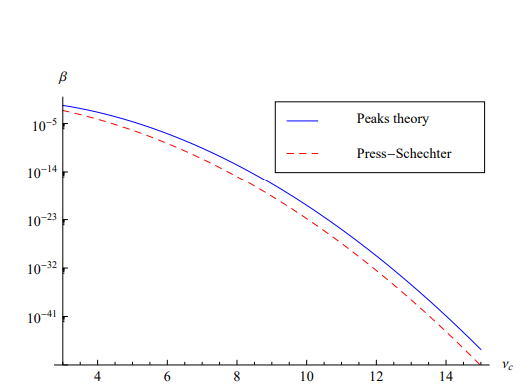
\includegraphics[width=0.7\textwidth]{Peaksvspress.png}
    \caption{The  Value of $\beta$ calculated using Press-Schechter or Peaks theory against $\nu_c = \delta_c/\sigma$. Taken from \cite{Young_2014} }
    \label{fig:3.1}
\end{figure}

Figure \ref{fig:3.1} illustrates the difference between the predicted values for each computation. While $\nu$ is not too large, the two are in fairly close agreement (varying by a factor of order 10). The difference between $\beta {peaks}$ and $\beta_{PS}$ is consistently higher for larger values of $\nu_c$. The error caused by the uncertainty in the threshold value $\delta_c$, however, overpowers the difference between both methods.\\
The mass variance in radiation domination(w = 1/3) is given by
\begin{align}
    \sigma^{2}(R) = \frac{16}{81} \int_{0}^{\infty} \,\frac{dk}{k}  \Tilde{W}^{2}(R,k) (kR)^4\mathcal{P}_{\mathcal{R}_{c}}(k).  \label{3.34}
\end{align}
where $ \Tilde{W}^{2}(R,k)$ is the Fourier transform of the window function used to smooth the density contrast on a comoving scale R($\approx 1/(a_{form} H_{form}) = 2GM/a_{form} \gamma^{_1}$),$\mathcal{P}_{\mathcal{R}_{c}}(k)$ is the power spectrum of the primordial comoving curvature perturbation. We saw before that the power spectrum explains the amplitude of the density perturbations on different scales at some initial time. We define a "Transfer function"\footnote{Appendix \ref{Transfer function}} that modifies this primordial power spectrum and describes the evolution of the density perturbations on subhorizon scales.  So we can re-write Eq.\ref{3.34} as
\begin{align}
    \sigma^{2}(R) = \frac{16}{81} \int_{0}^{\infty} \,\frac{dk}{k}  \Tilde{W}^{2}(R,k) (kR)^4\mathcal{P}_{\mathcal{R}_{c}}(k) T^{2}(kR/\sqrt{3}).  \label{3.35}
\end{align}
We assume $\sigma(R) \ll 1$ which enables us to translate the constraint on $\beta$ into the constraint on $\nu_{c}$ which corresponds to the amplitude of the density fluctuation from the above equation. It would also provide directions for creating successful inflationary models with PBH formation. For example, if the constraint on $f$ for $30 M_\odot$ would be obtained as $f_{pbh} < 10^{-3}$, which is equivalent to $\beta < 3 \times 10^{-11}$ it could be interpreted as $\nu_{th} \gtrsim 6.46$, that is , that is, $\sigma \lesssim 0.08$ with $\delta_{c} = 0.5 $.
% \section{Monochromatic vs Extended}
% In the previous discussion to find the abundance of PBH, we considered a monochromatic mass function which serves as a good starting point for considering models which have a narrow spread of mass like the axion-curvaton model \cite{Kasuya_2009}. However, in a more realistic situation, the analysis can be extended to the case in which the PBH has an extended mass spectrum. An approach to represent it as shown in Ref. \cite{Carr:2016drx} is to integrate the differential mass function $\dv{n}{M}$ over a mass window of width $M$ at each $M$, which gives us the continuous function
% \begin{align}
%     n(M) =  M \dv{n}{M} = \dv{n}{ln M} \label{3.36}
% \end{align}
% $n(M)$ is interpreted as the number density of the PBHs in the mass range$(M,2M)$. We can define the quantities corresponding to the mass density and dark-matter fraction, respectively, in the same mass range as
% \begin{align}
%     \rho(M) = M^{2} \dv{n}{M} , f(M) = \frac{\rho(M)}{\rho_{CDM}} \label{3.37}
% \end{align}
% This has the advantage of allowing one to see where the majority of the mass is right away and is analogous to splitting the mass up into bins. If the width of the mass function is less than M, the aforementioned representations are problematic. We have seen that one can always specify an effective value $f(M)$ at each mass scale if one considers an extended mass function to be one with a width greater than $M$. Although it is simple if the mass function is a delta function (ie. exactly monochromatic), the issue for monochromatic mass functions is typically more challenging. If it is almost monochromatic, or if its width is $(\Delta (M) \ll M)$, then there is an issue.\\
% The mass function should only be very extended if the PBHs are formed from precisely scale-invariant density fluctuations, even if a perfectly monochromatic mass spectrum is obviously not physically feasible. This has the critical implication that a constraint on one mass scale may also imply a constraint on nearby scales. We noted that the monochromatic assumption fails miserably if PBHs develop through critical collapse, and Ref \cite{Yokoyama:1998xd} has discussed how this modifies the shape of $\beta(M)$.
%%%%%%%%%%%%%%%%%%%%%%%%%%%%%%%%%%%%%%%%%%%%%%%%%%%%%%%%%%%%%%%%%%%%%%%%%%%%%%%%%%%%%%%%%%%%%%%%%%%%%%%%%%%%%%%%%%%
\section{Models of Inflation for PBH generation}
In the previous chapter, we discussed how inflation provides a mechanism for generating primordial perturbations via quantum fluctuations of a scalar field and the aspects which are relevant to the formation of PBH. In the standard single slow-roll inflation, the slow-roll parameter is anticipated to suppress the higher-order cumulants. However, non-standard inflationary models that violate the slow-roll condition must be taken into consideration for effective PBH formation which will be discussed in this section.\\
We have observed that PBH arises when an overdense region enters the Hubble horizon. If these regions are sourced by the primordial curvature perturbations, then the size of the overdense region should be determined by the comoving wavenumber, $k$ of the primordial perturbations. So, we can obtain a relation between the Hubble Scale at the PBH formation and the comoving wavenumber of the sourced primordial curvature perturbation as $k =aH_{|formation}$.
During radiation era $aH \propto a^{-1}$, hence we can write the relation between comoving wave number and the Hubble parameter at the formation as $H_{form} \propto k^2$, which we can substitute in the Eq. \ref{3.12} for $M$. So, we get a relation between the mass of PBHs and the comoving wavenumber as \cite{Sasaki_2018}


\begin{align}
    M(k) & =\left.\gamma \frac{4 \pi}{3} \rho H^{-3}\right|_{k=a H} =\gamma M_{eq}\left(\frac{g_{* eq}}{g_*}\right)^{1 / 6}\left(\frac{k_{eq}}{k}\right)^2 \label{3.36}
\end{align}

where $M_{eq}$ denotes the horizon mass at the matter radiation equality calculated as,
\begin{align}
    M_{eq}=\frac{4 \pi}{3} \rho_{eq} H_{eq}^{-3}=\frac{8 \pi}{3} \frac{\rho_r^0}{a_{eq} k_{eq}^3} \label{3.37}
\end{align}

We have used an approximation that the effective d.o.f. for energy density $g_*$ is almost equal to that for entropy density $g_{*s}$. Using $\rho_r^0=7.84 \times 10^{-34}g cm^{-3}$, $k_{eq}=0.07 \Omega_k h^2 Mpc^{-1}, a_{eq}^{-1}=24000 \Omega_k h^2$, and $g_{eq}=$ 3.36, we can finally obtain 
\begin{equation}
    M(k)=30 M_{\odot}\left(\frac{\gamma} {0.2}\right)\left(\frac{\left.g_*\right|_{k=a H}}{106.75}\right)^{-1 / 6}\left(\frac{k}{2.9 * 10^{5} Mpc^{-1}}\right)^{-2} \label{3.38}
\end{equation}
Inferring precedence between the observable scales via CMB measurements and $30 M_{\odot}$ PBHs from the above equation using the pivot scale as mentioned in Planck 2015\cite{Planck:2015fie} as a typical observable scale by CMB observations, $k_{CMB}$ we see that
\begin{align}
    \mathcal{N}_{CMB -30M{\odot} PBHs} = \ln\qty(\frac{k_{30M_{\odot} PBHs}}{k _{CMB}}) = \ln \qty(\frac{2.9 \times 10^{5} \text{Mpc}^{-1}}{0.002 \text{Mpc}^{-1}}) \sim 20, \label{3.39}
\end{align}

On the other hand, it is necessary for there to be a minimum of 50-60 e-folds between the time the existing horizon scale leaves the Hubble horizon and the end of inflation.
As a result of the preceding discussion, we infer that if we wish to create $30M_{\odot}$ PBHs from the perturbations of the primordial density, we need to take into account any mechanism that can amplify the perturbations during the inflationary phase.


%%%%%%%%%%%%%%%%%%%%%%%%%%%%%%%%%%%%%%%%%%%%%%%%%%%%%%%%%%%%%%%%%%%%%%%%%%%%%%

\subsection{Single Field Inflation}
In the standard slow roll inflation scenario the power spectrum form is written as \ref{2.148} (with the parameters $\alpha_s$ and $\beta_s$ suppressed) as:
\begin{align}
    \mathcal{P}_{\mathcal{R}_c}(k) = A_{\mathcal{R}_c}\qty(\frac{k}{k_{*}})^{n_s - 1}, \ \label{3.40}
\end{align}
where $n_s -1 $ can be written in terms of the slow-roll parameters( $\eta$ (Eq.\ref{2.36}) and $\epsilon$ (Eq.\ref{2.41})) as shown in Eq. \ref{2.149}.
For successful inflation, the condition to be satisfied is $\eta,\epsilon \ll 1$. Let us see if the spectral index satisfies the condition. \\
From the latest CMB observation, it is indicated that $P_{R_c} \approx 10^{-9}$(COBE normalization) over the CMB observable scales and the effects of PBH formation is quite effective to have a point of interest for  $\mathcal{P}_{\mathcal{R}_c}  = \mathcal{O}(10^{-2} - 10^{-1})$. So, for realizing such a large amplitude at $k = k_{30M_{\odot} PBHs} = 2.9 \times 10^5 \mathrm{MPc^{-1}}$ with a blue tilted power spectrum (large amplitude for small scale i.e large comoving number) consistent with the COBE normalization, we need \cite{Sasaki_2018}

\begin{align}
    n_s - 1 = \ln \qty(\frac{\mathcal{P}_{\mathcal{R}_c}(k_{30M{\odot} PBHs})}{\mathcal{P}_{\mathcal{R}_c}(k_{CMB})})/ \ln\qty(\frac{k_{30M_{\odot} PBHs}}{k_{CMB}}) \simeq 0.85 \label{3.41}
\end{align}
From the obtained value we observe that the spectral index value obtained from CMB observations like the Planck observation, we have 
\begin{align}
    n_s = 0.968 \pm 0.006 \text{at} k_{*} = 0.05 \mathrm{Mpc^{-1}}\label{3.42}
\end{align}
Hence, for PBH the standard inflationary model conflicts with the CMB observations even if we implement the blue-tilted power spectrum.

%%%%%%%%%%%%%%%%%%%%%%%%%%%%%%%%%%%%%%%%%%%%%%%%%%%%%%%%%%%%%%%%%


\subsection{Running  Mass Inflation}
 The formation of PBH in the running mass inflation model is one of the possibilities to realize a relatively large blue-tilted inflationary model consistent with the Planck results. the inflationary potential is defined in this case as 
 \begin{align}
     V(\varphi) = V_{0} + \frac{1}{2}m_{\varphi}^{2}(\varphi)\varphi^{2} \label{3.43}.
 \end{align}
The significant dependency of the $\eta$ on time during inflation in this model suggests that the scale dependence of the $n_s$ may also become large. Thus, when $\eta$ remains to be small to be consistent with the Planck result on CMB scales, but $\eta$ takes a positive larger value on smaller scales, we can realize the large
 amplitude of primordial curvature perturbations on an appropriately small scale which could be seeds of PBHs. The primordial power spectrum for these types of models incorporates the scale-dependence of the spectral index perturbatively rather than being a simple power law as mentioned in Eq. \ref{2.148}. Let us rewrite it below
 \begin{align}
    \mathcal{P}_{\mathcal{R}_c}  = A_s (\frac{k}{k_0})^{n_s -1 + \frac{1}{2}\alpha_{s} ln(k/k_0)+ \frac{1}{3!}\beta_{s}ln^2(k/k_0) + ....}, \label{3.44} 
 \end{align}
Where $\alpha_{s}$ and $\beta_{s}$ are the "running spectral index" and "running of running" parameters, which are greatly suppressed during slow-roll inflation but are very significant in this model. Ref. \cite{Sasaki_2018} discussed that for the above parameterization to produce $30M_{\odot} \mathrm{PBHs}$\footnote{Focusing on inflation models producing PBHs of $\mathcal{O}(1-10)M_{\odot}$} with $n_s = 0.968$ on CMB scales, $\alpha_{s}$ needs to be taken to be about 0.1.
 It was further addressed that for such a large $\alpha_{s}$ and assuming negligibly small $\beta_s$, PBH with smaller masses would be overproduced. To avoid this overproduction a cutoff in the primordial power spectrum at an appropriate scale is needed, which is realized by taking into account the non-negligible "running of running" parameters $\beta_s$. 
%%%%%%%%%%%%%%%%%%%%%%%%%%%%%%%%%%%%%%%%%%%%%%%%%%%%%%%%%%%%%%%%%%%%%%%%%%%%%%%%%%%%%%%%%%%%%


\subsection{Multifield}
In this section, we will briefly discuss some multi-field scenarios that can generate large primordial curvature perturbations with large amplitudes.
\subsubsection{Double Inflation}
A peak in the primordial power spectrum can be realized at an appropriate scale if the inflaton experiences a period during inflation where it temporarily slows down. This corresponds to a very flat region in the inflationary potential, as we have mentioned in the single-field inflation scenario. The temporal violation of the conventional slow-roll conditions is crucial in the aforementioned models for realizing the enhancement of primordial curvature perturbations to form PBHs during the inflationary era. This case of features can be readily achieved in the Multi-Scalar models. In double inflation, there are two separate periods of inflation, with
perturbations on cosmological scales being generated during the first period and those on small scales during the second. Hybrid inflation models with a mild waterfall transition, which will be discussed next, fall into this class. 
\subsubsection{Hybrid Inflation}
A detailed description of Hybrid inflation can be found in reference \cite{PhysRevD.54.6040} \cite{PhysRevD.92.023524}. Hybrid inflation is the most commonly studied two-field model in the context of PBH production. $\varphi$ is one of the fields that slow-rolls whereas the other field $\psi$'s false vacuum energy  drives the accelerated expansion. There is a phase transition that takes place at a critical value of $\varphi$ with $\psi$ undergoing a waterfall transition to a global minimum and the inflation stops. There are large quantum fluctuations around the phase transition which generates spikes in the power spectrum on small scales, which leads to a large abundance of light PBH. There can be some parameter values for which the waterfall transition is 'mild' so that there is a 2nd phase of inflation as the field $\psi$ evolves to the minimum of its potential. In this instance, isocurvature perturbations are produced at the first stage of the waterfall transition, when both fields are significant, and this causes a large peak in the curvature perturbation power spectrum. At the first stage of inflation, perturbations on cosmological scales are produced and may be consistent with CMB observations.\\


\subsubsection{Curvaton Model}
For producing primordial curvature disturbances that can result in the production of primordial black holes, the curvaton scenario offers an alternative to the single field inflationary model (PBHs). The inflaton, which causes inflation, and the curvaton, which causes the perturbations in primordial curvature, are the two scalar fields involved in the curvaton scenario. As the curvaton field begins to oscillate and behave as non-relativistic matter during the radiation-dominated epoch, the curvaton field initially causes isocurvature perturbations, which eventually turn into adiabatic curvature perturbations. The adiabatic curvature perturbations become constant in time when the curvaton eventually decays into radiation\cite{Lyth_2005}. In order to produce the huge amplitude fluctuations required for PBH creation on small scales while maintaining consistency with the CMB measurements on larger scales, the curvaton fluctuations exhibit a scale-invariant feature on smaller scales and a cutoff on a larger scale. On super-Hubble scales, multiple curvaton fields can intensify the curvature perturbations, producing a large number of PBHs up until the enhancement stops. For example "axion-like curvaton\cite{PhysRevD.87.063519}".











%%%%%%%%%%%%%%%%%%%%%%%%%%%%%%%%%%%%%%%%%%%%%%%%%%%%%%%%%%%%%%%%
%%%%%%%%%%%%%%%%%%%%%%%%%%%%%%%%%%%%%%%%%%%%%%%%%%%%%%%%%%%%%%%%
%%%%%%%%%%%%%%%%%%%%%%%%%%%%%%%%%%%%%%%%%%%%%%%%%%%%%%%%%%%%%%%%




\section{Exploring Limitations in Simplified Models of Primordial Black Hole Formation} \label{limtiation}
In our previous discussion to find the abundance of PBH, we considered a monochromatic mass function with a mass similar to the horizon mass at the creation and that the PBHs arise from the collapse of overdensities that are spherical and have a Gaussian distribution which serves as a good starting point. However, this oversimplified model can result in misinterpretation of observational constraints. As a result,  a more realistic portrayal of the formation process is required, especially as the constraints on the allowed PBH density at each epoch have become more precise. Additionally, The potential existence of intermediate-mass PBHs has also been suggested by recent observations \cite{2016PhRvL.116t1301B}, which emphasizes the need for a more exact description of PBH production.
\subsection{Precise Threshold Value}
The estimated threshold density perturbation for PBH formation is approximately 1/3 according to Eq. \ref{3.8}, but more precise values have been obtained through extensive research involving numerical simulations and analytical calculations. A formula in Ref. \cite{Harada_2013} gives a close estimate of the threshold as
\begin{align}
    \Tilde{\delta}_c =[3(1+w)/(5+3w)] \sin ^2[\pi \sqrt{w} /(1+3 w)], \label{3.45}
\end{align}
where $\Tilde{\delta}_c$ is the amplitude measure used in
numerical simulations and
\begin{align}
    \delta_{H c}^{UH}=\sin ^2[\pi \sqrt{w} /(1+3 w)] ,\label{3.46}
 \end{align}
 where $\delta_{H c}^{UH}$ is the amplitude of the density perturbation at horizon crossing in the uniform Hubble slice and $w$ is the equation of state of the dominant component in the Universe at the formation. However, it has been found that the threshold is not fixed as different density or curvature perturbation profiles can collapse to form PBHs above different thresholds, which makes physical sense. The range of the threshold's spread, measured in terms of the comoving density perturbation, is from 0.3 to 0.66. It's interesting to note that the rough estimate of 1/3 is included in this range.
 %%%%%%%%%%%%%%%%%%%%%%%%%%%%%%%%%%%%%%%%%%%%%%%%%%%%%%%%%%%%%%%%%%%%%%%%%%%%%%%%%%
 \subsection{Critical Collapse}

\hspace{0.5cm}Previously, it was assumed that an overdensity that enters the horizon and collapses to a black hole with a mass of the order of the horizon mass $M_{H}$ would do so immediately. However, it has since been shown that when considering spherical symmetry, the relationship between the black hole mass $M_{BH}$ and the overdensity $\delta$ at horizon crossing and the horizon mass $M_{H}$ follows a critical scaling relation described by equation 
 \begin{align}
     M_{BH} = \kappa M_{H}(\delta -\delta_{c})^\gamma \label{3.47},
 \end{align} 
 This scaling relation includes a constant $\kappa$, a threshold overdensity $\delta_{c}$, and a critical exponent $\gamma$ that depends on the fluid containing the overdensity at horizon crossing \cite{Musco_2013}. The scaling relation in Eq. \ref{3.47} was confirmed  through numerical work in Ref. \cite{Musco_2013}. They also showed that the critical exponent $\gamma$ is independent of the perturbation profile, however, $\delta_{c}$ and $\kappa$ may depend on the perturbation profile.\\

When applying this critical collapse model to primordial black hole formation, it was found that the horizon-mass approximation was still valid at the time of formation. However, this conclusion was based on the assumption that the primordial black hole mass function was monochromatic. Further study has revealed that the inclusion of critical collapse can cause a significant shift, lowering, and broadening of the primordial black hole mass spectra by several orders of magnitude when a realistic model of the power spectrum underlying their production is taken into account. These small effects should be taken into account to obtain precise constraints on inflationary models. This has been demonstrated for a variety of inflationary models in Ref. \cite{K_hnel_2016}.
%%%%%%%%%%%%%%%%%%%%%%%%%%%%%%%%%%%%%%%%%%%%%%%%%%%%%%%%%%%%%%%%%%%%%%%%%%%%%%%%%%%%%%%
\subsection{Non-sphericity of the Overdense Region}
In our previous discussion, we considered an isolated spherically symmetric perturbation as a criterion for PBH formation, which is a reasonable first approximation and makes our calculation easier. In reality, this is not the case and the effects of non-sphericity might be consequential even if in most cases the initial non-sphericity is either small or eventually leads to spherical objects. One of the most simple and spherically deviated overdense regions is approximated as an ellipsoid. The approximate threshold value for ellipsoid collapse is 
\begin{align}
    \frac{\delta_{ec}}{d_c} = 1 + \kappa \qty(\tall \frac{\sigma^2}{\delta_{c}^2})^{\gamma} \label{3.48}
\end{align}
where $d_c$ is the threshold for the spherical collapse,$\sigma^2$ is the amplitude of the density power spectrum at a given scale, and $\kappa$ and $\gamma$ are constants to be found numerically.
\cite{Kuhnel:2016exn}, it was stated that to estimate the modification of the threshold in the case of the non-spherical overdense region that was approximated as an ellipsoid, it was demanded that a spherical region enclosed by the shortest axis of the ellipsoid satisfies the collapse criterion for the spherical overdensity. The collapse along the longer axes follows, moving faster than linearly, as the collapse condition. They considered a Gaussian-distributed overdensity and showed that the expectation value for the shape of densities as
\begin{align}
    \langle e \rangle = \frac{3\sigma}{\sqrt{10\pi} \delta}\label{3.49}
\end{align}
Furthermore, they assumed that the ellipsoid is of uniform density and that the density profile in the central region is higher. Thus, given this simplistic analysis, they discover that$\gamma = 1/2 $ and $\kappa = (9\pi \sqrt{10})$.
They discovered that the non-sphericity effects would raise the formation threshold, which would suppress the mass spectrum generally. Although the exact amount of non-sphericity-related suppression is unsure, the mass spectrum's functional shape remains unaltered. However, it should be noted that  Eq. \ref{3.49}, does not provide the ellipticity for non-Gaussian overdensities, therefore it is important to consider how these two effects interact.

%%%%%%%%%%%%%%%%%%%%%%%%%%%%%%%%%%%%%%%%%%%%%%%%%%%%%%%%%%%%%%%%%%%%%%%
\subsection{Non-Linear effects}

The energy density profile in Eq. \ref{3.4} for radiation dominated universe($w = 1/3$) can be (re)written as
\begin{align}
    \delta(\vec{x}, t)=-\frac{4}{9} (\frac{1}{aH})^{2} e^{-2 \zeta(\vec{x})}\left[\nabla^2 \zeta(\vec{x})+\frac{1}{2} \partial_i \zeta(\vec{x}) \partial^i \zeta(\vec{x})\right] \label{3.50}
\end{align}
We can notice from the above equation that the relation between the overdensity and the curvature perturbation is intrinsically non-linear and we obtain a linear relation only under the condition that both the $\zeta$-curvature and curvature gradients are small $\left(\left|\zeta\right|,\left|\nabla \zeta\right| \ll 1\right)$. In particular, in Eq  \ref{3.50} it is often assumed that the exponential damping $e^{2 \zeta}$ (effects the peak of the profile) and the quadratic gradient correction $\left(\nabla \zeta \cdot \nabla \zeta\right)$ (effects the tail of the profile) can be neglected, effectively linearising the relation between $\zeta$-curvature perturbation and the overdensity perturbation $\delta^{\text {LIN }} \propto \nabla^2 \zeta$


Even if the linear approximation is accurate at the beginning, non-linearities have already had a big impact by the time the horizon is crossed since both curvature and overdensity perturbations are of order unity. When assessing PBH abundance, numerical simulations of PBH formation and  cosmological connections, neglecting the non-linearities have a substantial impact. This topic has been extensively covered by Kalaja \emph{et al}\cite{Kalaja:2019uju}. \\
They demonstrate that, depending on the shape of the perturbation, applying a linear approximation significantly underestimates the real size of the perturbation (and hence the mass contained in the horizon) by a factor of up to $\sim$ 6: Most noticeably impacted are perturbation profiles that are steeper. \\
They also compare some key quantities with the full non-linear equation(NL)  with their corresponding linear approximation(LIN). For example, they showed that  linearisation underestimates the typical scale of perturbation. Under linear approximation, the typical scale of the perturbation is $r_t^{\mathrm{LIN}}=\hat{r}_k$, which is to be compared against the typical non-linear scale $r_t^{\mathrm{NL}}=\hat{r}_k e^{-\zeta\left(\hat{r}_k\right)}$. Since $\zeta$ is negative, linearisation underestimates the real size of the perturbation, i.e., $r_t^{\mathrm{LIN}} / r_t^{\mathrm{NL}}<1$. \\
Now, since in radiation-domination the comoving horizon scales as $r_{\text {H }} \propto t^{1 / 2}$ and the horizon crossing condition is $a_k H_k r_t=1$, linearisation also underestimates the horizon crossing time $t_k$  and since the inferred mass of the PBH is also affected by linearisation through a different estimate of the horizon crossing time as seen in Eq. \ref{3.47} where $M_{H}(t) = (2H)^{-1}$, the main effect is that the linear approximation underestimates the mass inside the horizon:
\begin{align}
    \frac{M_{\text {hor }}^{\mathrm{LIN}}}{M_{\text {hor }}^{\mathrm{NL}}}=\frac{t_k^{\mathrm{LIN}}}{t_k^{\mathrm{NL}}}=\left(\frac{r_t^{\mathrm{LIN}}}{r_t^{\mathrm{NL}}}\right)^2<1 .\label{3.51}
\end{align}
Another significant aspect that was highlighted was the importance of nonlinearity in the smoothing process.
To account for spatial curvature, which introduces certain nuances, it is advised that filtering be done in physical coordinates rather than comoving coordinates, as in linear theory. However, when the spatial curvature is introduced into the filtering procedure, and the full non-linear relation between the non-linear overdensity and curvature is used, filtering the overdensity fields or curvature is no longer equivalent, implying that filtering $\zeta$ is not equivalent to filtering $\delta$ in the non-linear case. Furthermore, it was discussed that because of the non-linearity between overdensity and curvature, the two-point functions of the overdensity field receive contributions from all of the n-point functions of the $\zeta$ -curvature field, implying the importance of non-Gaussianity when going beyond the linear approximation. (For more details refer to Ref. \cite{Kalaja:2019uju}). 
%%%%%%%%%%%%%%%%%%%%%%%%%%%%%%%%%%%%%%%%%%%%%%%%%%%%%%%%%%%%%%%%%%%%%%%%%%%%%%%%%%%%%%%%%
\subsection{Non-Gaussianity}
PBHs are formed from the extremely high-density tail of the spectrum of fluctuation, and their abundance is significantly affected by any  non-gaussianity in the density perturbation profile.
The way the perturbations are created, which is determined by the inflationary models, determines the impact of non-Gaussianity on the calculation of the perturbations to the primordial curvature and can alter the initial mass fraction PBHs in a major way.\\
 
In this section, we will follow Ref. \cite{Franciolini:2018vbk}  where they discuss the role of non-gaussianity in determining the PBH mass-fraction at formation time by using a path integral formulation \cite{Matarrese:1986et}. However, instead of going into too much detail, we will focus on discussing the main findings and results of the study(for detailed calculation refer to \cite{Franciolini:2018vbk}).

The probability for a single-density contrast  $\zeta_{R}$ to be above the threshold $\zeta_{c}$ for it to collapse and form a black hole can be directly calculated by evaluating the one-point threshold statistics and it is given by
\begin{align}
    P\left(\zeta_{R}>\zeta_{c}\right)=\left\langle\rho_{\nu, R}(\vec{x})\right\rangle & =\left\langle\Theta\left(\zeta_{R}(\vec{x})-\nu \sigma_{R}\right)\right\rangle = h_{0}(\nu)+\frac{e^{-\nu^{2} / 2}}{\sqrt{2 \pi}} \sum_{n=3}^{\infty} \frac{1}{2^{\frac{n}{2}} n !} \Xi_{n}(0) H_{n-1}\left(\frac{\nu}{\sqrt{2}}\right), \label{3.52}
\end{align}
for a more detailed description refer to Ref. \cite{Franciolini:2018vbk, Matarrese:1986et}.
Eq. \ref{3.52} is the exact solution without any approximations. For large threshold, i.e $\nu \gg 1$ using the asymptotic behaviour of Hermite polynomials and the complementary error function 
\begin{align}
    \begin{aligned}
        & H_{n}\left(\frac{\nu}{\sqrt{2}}\right)=2^{\frac{n}{2}}                \nu^{n}\left(1+\mathcal{O}\left(\nu^{-2}\right)\right) \\
        & h_{0}(\nu)=\frac{1}{2} \operatorname{Erfc}\left(\frac{\nu}{\sqrt{2}}\right)=\frac{e^{-\nu^{2} / 2}}{\sqrt{2 \pi \nu^{2}}}\left(1+\mathcal{O}\left(\nu^{-2}\right)\right),\label{3.53}
    \end{aligned}
\end{align}
Eq. \ref{3.52} reduces to
\begin{align}
    P\left(\zeta_{R}>\zeta_{c}\right)=\frac{e^{-\nu^{2} / 2}}{\sqrt{2 \pi \nu^{2}}} \exp \left\{\sum_{n=3}^{\infty} \frac{(-1)^{n}}{n !} w_{R}^{(n)}(0) \nu^{n}\right\}=\frac{1}{\sqrt{2 \pi \nu^{2}}} \exp \left\{-\nu^{2} / 2+\sum_{n=3}^{\infty} \frac{(-1)^{n}}{n !} \xi_{R}^{(n)}(0)\left(\zeta_{c} / \sigma_{R}^{2}\right)^{n}\right\}, \label{3.54}
\end{align}

The argument (0) signifies that all the points have to be taken coinciding with each other. On taking the smoothing radius to be $R_{H}$ we can see that the expression gives the primordial mass fraction $\beta$ with the approximation of $\nu \gg 1$. Another interesting thing to notice is that, when the higher order $(n > 2)$ linked correlators vanish, it is possible to identify the leading order term that produces the Gaussian outcome.
Let's now look at how Eq. \ref{3.54} is used to analyze the effects of non-Gaussianity and how important it is to evaluate whether higher-order correlators that incorporate the non-Gaussian corrections are significantly impacting the computation of abundance in a given model.\\
Taking inspiration from the notion of fine-tuning we see how sensitive $\beta(M)$ is to the various dimensionless quantities, the cumulants, which are defined by the relation
\begin{align}
    S_n=\frac{\xi_{\nu, R_H}^{(n)}(0)}{\left(\xi_{\nu, R_H}^{(2)}(0)\right)^{n-1}}=\frac{\langle\overbracket{\zeta_{R_H}(\vec{x}) \cdots \zeta_{R_H}(\vec{x})}^{n \text {-times }}\rangle}{\sigma_{R_H}^{2(n-1)}}, \label{3.55}
\end{align}
Now, the fine-tuning parameter $\Delta_{n}$ which is the logarithmic variation of the PBH abundance after introducing the n-th cumulant is defined as
\begin{align}
    \Delta_{n}=\frac{\mathrm{d} \ln \beta_{\operatorname{prim}}(M)}{\mathrm{d} \ln S_{n}} \label{3.56}
\end{align}
In the presence of the $n^{th}$ cumulant, the non-Gaussian PBH abundance Eq. \ref{3.52} is related to the Gaussian abundance in terms of the correction parameter as
\begin{align}
    \frac{\beta_{\text {prim }}^{\mathrm{NG}}(M)}{\beta_{\text {prim }}^{\mathrm{G}}(M)}=e^{\Delta_{n}} ,\label{3.57}
\end{align}
From the above Eq. \ref{3.57} we can tell that the resulting PBH abundance is exponentially sensitive to deviation from Gaussianity unless 
$
\left|\Delta_{n}\right| \lesssim 1
$
\\

Using, the Gaussian mass fraction $\beta_{G} \simeq \sqrt{\frac{1}{2\pi\nu^{2}}}e^{-\nu^{2}/2}$ and Eq. \ref{3.54} we find that
\begin{align}
    \left|\Delta_{n}\right|=\frac{1}{n !}\left(\frac{\zeta_{c}}{\sigma_{R_{H}}}\right)^{2}\left|S_{n}\right| \zeta_{c}^{n-2} \label{3.58}
\end{align}
The above equation demonstrates that non-Gaussianity modifies the Gaussian prediction for the PBH abundance exponentially unless
\begin{align}
    \left|S_{n}\right| \lesssim\left(\frac{\sigma_{R_{H}}}{\zeta_{c}}\right)^{2} \frac{n !}{\zeta_{c}^{n-2}} \label{3.59}
\end{align}
Franciolini \emph{et al}\cite{Franciolini:2018vbk} analysed the restrictiveness of the above condition Eq. \ref{3.59} in the case of PBH from the single field inflation model and the axion-curvaton model(presence of a spectator field). Following Ref. \cite{Motohashi:2017kbs}, they set $\beta(M)$ to correspond to the total amount of dark matter that exists today in the form of PBHs and look for the effects of non-Gaussianity. They find the non-Gaussian results in the cases of the single-field model and the axion-curvaton model are smaller by about ten and twenty orders of magnitude respectively than the Gaussian results, indicating the sensitivity of the cosmological predictions to the non-Gaussianity. Their findings further demonstrate how non-Gaussian corrections affect the PBH's clustering features, which in turn influences PBH merger and may have an impact on PBH cosmic evolution.




    



,
\chapter{Statistical Analysis of Random Cosmic Field}\label{stats}
\justifying
\section{Random fields} \label{section 3.1}
A significant challenge in modern cosmology is identifying appropriate tools to analyze the distribution of density fluctuations, their initial conditions, and their subsequent evolution. The current explanation for the large-scale structure of the Universe posits that the present distribution of matter on cosmological scales results from the growth of primordial, small seed fluctuations in an otherwise homogeneous Universe, amplified by gravitational instability.\\

Testing cosmological theories that characterize these primordial seeds is inherently statistical rather than deterministic. This is due to the lack of direct observational access to primordial fluctuations, which would provide definite initial conditions for deterministic evolution equations. Moreover, the timescale for cosmological evolution far exceeds the period over which we can make observations, preventing us from following the evolution of individual systems. Instead, we observe different objects at various stages of their evolution through our past light cone.\\

The observable Universe is modelled as a stochastic realization of a statistical ensemble of possibilities. The objective is to make statistical predictions based on the properties of the primordial perturbations that lead to the formation of large-scale structures. According to the cosmological principle, which asserts that the Universe is homogeneous and isotropic on large scales, cosmological models assume that the statistical properties of density fluctuations are uniform across widely separated regions of the Universe.\\

A crucial assumption in cosmology is that the observable part of the Universe is a fair sample of the whole. This implies that statistical measures, such as correlation functions, should be considered averages over the ensemble. However, we only have one realization of the Universe. The fair sample hypothesis posits that samples from well-separated regions of the Universe are independent realizations of the same physical process, and there are enough independent samples in the observable Universe to be representative of the statistical ensemble. The hypothesis of ergodicity further states that averaging over many realizations is equivalent to averaging over a sufficiently large volume. \cite{verde2008practicalguidebasicstatistical}\cite{Bernardeau_2002}\\

Theories are limited to predicting the statistical characteristics of the density contrast $\delta(x)$. The cosmological principle requires that this density contrast forms an isotropic and homogeneous random field, of which the observable Universe is one realization. Among the models explaining the large-scale structure of the Universe, those based on the inflationary paradigm are most widely considered. In the simplest single-field models, these generate adiabatic, Gaussian initial fluctuations, with the origin of stochasticity lying in quantum fluctuations generated in the early Universe.\\

In cosmology, the scalar field $\delta(x)$ suffices to define the initial fluctuations field and, ideally, the current matter and galaxy distribution. Identifying the right tools to analyze the distribution of density fluctuations, their initial conditions, and their evolution is a major challenge in the study of cosmic structures. In the following sections, we will discuss some of these tools in detail.


For a cosmic random field, such as matter density, the infinite volume condition of the ergodic hypothesis is not satisfied, due to the limited size of the observable Universe. In this case, the ensemble average of an observable overall realization is equal to the spatial average. This means that the ensemble average of any cosmological quantity will be an estimator of its true value. The expectation value of the n-point correlation function (=i.e. the $n^{th}$ central moment for a multivariate joint probability density distribution of the density field $\rho(\mathbf{x})$ is defined as \cite{gnedenko1998theory}.


\begin{align*}
    \left\langle\left(\rho\left(\mathbf{x}_{1}\right)-\rho_{0}\right)\left(\rho\left(\mathbf{x}_{2}\right)-\rho_{0}\right) \ldots\left(\rho\left(\mathbf{x}_{n}\right)-\rho_{0}\right)\right\rangle & =\int_{V}\left(\rho\left(\mathbf{x}_{1}\right)-\rho_{0}\right)\left(\rho\left(\mathbf{x}_{2}\right)-\rho_{0}\right) \ldots\left(\rho\left(\mathbf{x}_{n}\right)-\rho_{0}\right) \\
    & \times p\left[\rho\left(\mathbf{x}_{1}\right), \rho\left(\mathbf{x}_{2}\right), \ldots, \rho\left(\mathbf{x}_{n}\right)\right] \autolabel{}
\end{align*}


Here $\rho$ is the expectation value of the average density field and the integration is over the infinite volume. Then the  Fourier transformation of the joint probability density function is given by the characteristic function $M(t)$ as:


\begin{equation}
    M(t) = \langle \exp(t \rho) \rangle = \int P(\rho) e^{t \rho} \, d\rho
\end{equation}

Using the series expansion of the exponential function, we get:

\begin{equation}
    e^{t \rho} = \sum_{n=0}^{\infty} \frac{(t \rho)^n}{n!}
\end{equation}

Substituting this series expansion into the integral, we obtain:

\begin{equation}
    M(t) = \int P(\rho) \left( \sum_{n=0}^{\infty} \frac{(t \rho)^n}{n!} \right) \, d\rho
\end{equation}

Interchanging the order of summation and integration, we have:

\begin{equation}
    M(t) = \sum_{n=0}^{\infty} \frac{t^n}{n!} \int P(\rho) \rho^n \, d\rho
\end{equation}

The integral \(\int P(\rho) \rho^n \, d\rho\) represents the \(n\)-th moment of \(\rho\), denoted as \(\langle \rho^n \rangle\). Therefore, the characteristic function can be written as:

\begin{equation}
    M(t) = \sum_{n=0}^{\infty} \frac{t^n}{n!} \langle \rho^n \rangle
\end{equation}




where $\rho=\rho_{1}, \rho_{2}, \ldots, \rho_{n}$ is a vector. The expectation value of $\left\langle\rho^{n}\right\rangle$ is the raw moment, i.e. the expectation value for $\rho_{0}=0$, and it is related to the central moments through the binomial transformation. Taking logarithm of Eq. \ref{eq:3.2} we get the $n$-th cumulants as:


\begin{equation}
    \ln M(t)=\sum_{n=1} \frac{t^{n}}{n!}\left\langle\rho^{n}\right\rangle_{c} \autolabel{}
\end{equation}


Equating the two, after expanding the Maclaurin series of $\ln M(t)$, we can get the relationship between cumulants and central moments of the density random field. Lets us see the the one-point results for the first four:


\begin{align}
    & \langle\rho\rangle_{c}=\langle\rho\rangle \\
    & \left\langle\rho^{2}\right\rangle_{c}=\left\langle\rho^{2}\right\rangle-\langle\rho\rangle_{c}^{2} \\
    & \left\langle\rho^{3}\right\rangle_{c}=\left\langle\rho^{3}\right\rangle-3\left\langle\rho^{2}\right\rangle_{c}\langle\rho\rangle_{c}-\langle\rho\rangle_{c}^{3}  \autolabel{}\\
    & \left\langle\rho^{4}\right\rangle_{c}=\left\langle\rho^{4}\right\rangle-4\left\langle\rho^{3}\right\rangle_{c}\langle\rho\rangle_{c}-3\left\langle\rho^{2}\right\rangle_{c}^{2}-6\left\langle\rho^{2}\right\rangle_{c}\langle\rho\rangle_{c}^{2}-\langle\rho\rangle_{c}^{4},
\end{align}


For the overdensity field,  $\delta(\mathbf{x})$, these relations can be derived by normalizing with the average density. Since the first central moment of the random overdensity fluctuations is zero (i.e. $\langle\delta\rangle=0$ ), the above equations are significantly simplified.

 When working with multipoint correlation functions, it is important to consider all permutations of the random field between points. The cumulant is the fundamental statistical measure of interest since it represents a set of independent quantities that fully characterize the perturbations' probability distribution function (PDF). Cumulants are commonly referred to in the literature as connected correlation functions, a term derived from quantum field theory and Feynman diagrams eg.Fig. \ref{fig:2.1}. The covariance is the second-order cumulant, or two-point cumulant, while the variance is the first-order cumulant, or one-point cumulant (i.e., the diagonal component).\\

Now, most inflationary models predict a Gaussian distribution for the initial density fluctuations due to the quadratic nature of the action. In the multi-variant case, we have


\begin{equation}
    P\left[\delta\left(\mathbf{x}_{1}\right), \delta\left(\mathbf{x}_{2}\right), \ldots, \delta\left(\mathbf{x}_{n}\right)\right]=\frac{1}{\sqrt{2 \pi} \operatorname{det}(C)} \exp \left[\frac{1}{2} \delta_{i} C_{i j}^{-1} \delta_{j}\right] \autolabel{}
\end{equation}


where $C i j=\left\langle\delta_{i} \delta_{j}\right\rangle_{c}$ is the covariance and $\delta_{i} \equiv \delta\left(\mathbf{x}_{i}\right)$. Substituting the Gaussian PDF in the characteristic function, all the odd cumulants vanish while the even are obtained by the sum of the product of the ensemble averages of two-point correlators, with all possible combinations between the different positions. This is encoded in the Wick's theorem of quantum and classical field theories as


\begin{equation}
    \left\langle\delta_{1} \delta_{2} \ldots\right\rangle=\sum_{\text {pairings pairs }} \prod_{(i, j)}\left\langle\delta_{i} \delta_{j}\right\rangle_{c} \autolabel{}
\end{equation}


However, in the case of a primordial non-Gaussian(PNG) perturbation field, the even-order cumulants are non-zero which implies that these higher-order correlators are a direct indication of the departure from Gaussianity. However, in the case of LSS, non-zero higher-order cumulants are seen due to the non-linear nature of gravity, which induces couplings between different modes and one of the challenging tasks is to disentangle the PNG signals from the late time evolution. In contrast, CMB probes see fluctuations immediately, following decoupling, making them free of such nonlinear influences.

\section{ Two-point correlation function and power spectrum}
 As we saw in section \ref{section 1.7.5} the two-point correlation function of the density field is the ensemble average of $\delta$ at two different points. It is given by


\begin{equation}
    \left\langle\delta\left(\mathbf{x}_{1}\right) \delta\left(\mathbf{x}_{2}\right)\right\rangle=\left\langle\delta\left(\mathbf{x}_{1}\right) \delta\left(\mathbf{x}_{2}\right)\right\rangle_{c}=\xi(r), \autolabel{}
\end{equation}

and taking the Fourier transform of $\xi(r)$ we get to Eq. \ref{1.2.118}
where the quantity $P(k)$ is the Fourier coefficient of the two-point correlation function, called the power spectrum. We saw strictly positive for a continuous random field  $\delta(\mathbf{x})$ and it is non-zero only for equal and opposite wavenumbers. \\


Now, let us try to understand what the power spectrum actually measures and look into Eq. \ref{1.2.119}, which is the one-point second cumulant $(\xi(0))$ of the linear overdensity field and we write it here again,


\begin{equation}
    \sigma^{2}=\left\langle\delta^{2}(\mathbf{k})\right\rangle_{c}=\int \frac{d k}{2 \pi^{2}} k^{2} P(k) \autolabel{}
\end{equation}


From the equation, we see that the power spectrum characterizes the amplitude of the density fluctuations around the mean background value.

Now, we will define the smoothed linear matter density contrast $\delta_{R}$, over a radius $R(M)=\left(3 M / 4 \pi \bar{\rho}_{m}\right)^{1 / 3}$, as\footnote{In the above equation, $M$ is the mass originating from the matter inside the region of size $R(M)$ and $\bar{\rho}_{m}$ is the average density of the Universe at present time.}

\begin{equation}
    \delta_{R}(\mathbf{k}, z)=W_{R}(k) \delta(\mathbf{k}, z). \autolabel{}
\end{equation}

. A popular choice for the filter is $W_{R}(k)=3(\sin k R-k R \cos (k R)) /(k R)^{3}$, which is the Fourier transform of the spherical top-hat window function \footnote{\ref{Window function}}. Hence, we can write a smoothed linear power spectrum $P_{R}(k)$ as in Eq. \ref{eq:3.29}, where now $M(k, z)$ is replaced by $M_{R}(k, z)=W_{R}(k) M(k, z)$. The smoothed mass variance of the density field, at mass scale $M$, is defined as

\begin{equation}
    \sigma_{R}^{2}(z)=\left\langle\delta_{R}^{2}(\mathbf{k})\right\rangle_{c}=\frac{1}{2 \pi^{2}} \int k^{2} P_{R}(k, z) d k \autolabel{}
\end{equation}


For a density random field with a well-defined average (\(\rho > 0\)), it is evident that the mass variance must diminish towards zero as the radius \( R \) extends indefinitely (i.e., \( \lim_{R \to \infty} \sigma^2(R) = 0 \)). Consequently, the two-point correlation function must also approach zero for large separations (i.e., \( \xi(r \to \infty) \rightarrow 0 \)). This leads to the condition:

\begin{equation}
    \int d^3 r \, \xi(\mathbf{r}) = 0 \autolabel{}
\end{equation}

where the integral spans across all space. As a consequence, there exist distances \( r \) where \( \xi(r) < 0 \). Another significant property of the two-point correlation function, arising from the ergodicity of the density random field, is its maximum value at zero separation (i.e., \( \xi(0) > |\xi(\mathbf{r})| \)). Finally, Eq. (3.85) defines the correlation length as:

\begin{equation}
    r_{c}^{2} = \frac{\int dr \, r^2 |\xi(r)|}{\int dr \, |\xi(r)|} \autolabel{}
\end{equation}

This quantity characterizes how far correlations persist in the density fluctuation field, indicating the extent to which a localized perturbation influences the surrounding system.


\subsection{ Perturbative Expansion: up to one-loop}

In the previous chapter, we saw that the perturbative solution to the density and the velocity depended on the PT scheme we used, for the first-order (linear) fields. Now we will write the linear matter power spectrum using the linear part of the expansion. Using Eq \ref{eq:3.29} we get:


\begin{align*}
    & \left\langle\delta_{m}^{(1)}\left(\mathbf{k}_{1}\right) \delta_{m}^{(1)}\left(\mathbf{k}_{2}\right)\right\rangle_{c}=M\left(k_{1}, z\right) M\left(k_{2}, z\right)\left\langle\Phi\left(\mathbf{k}_{1}\right) \Phi\left(\mathbf{k}_{2}\right)\right\rangle_{c} \quad \Rightarrow \\
    & P_{m}^{L}(k, z)=M^{2}(k, z) P_{\Phi}(k) \autolabel{}
\end{align*}


where $\Phi$ is the primordial Bardeen gravitational potential, with a power spectrum given by,
\begin{equation}
    P_{\phi}(k) = \frac{9}{25}\frac{2\pi^{2}}{k^{3}} \mathcal{A}_{s}^{2}\left(\frac{k}{k_{0}}\right)^{n_{s}-1} \autolabel{}
\end{equation}
where we used Eqs. (\ref{1.2.120}, \ref{1.2.123} and \ref{eq:3.29}).
Here we have used in the perturbative solution the transfer function, incorporated through the Poisson relation of the linear density field with the primordial gravitational potential Eq. \ref{eq:3.31}. 

Now, we proceed to derive higher-order corrections to the linear power spectrum, from the perturbative solution of the matter and velocity fields which is done by using the perturbative expansion of a field and substituting it in the two-point correlation function Eq. \ref{1.2.113}. Keeping only the non-zero combinations, after taking into account the cumulant relation, results in a series of terms with an increasing power of the linear field. The terms that have the power of the linear solution to the $n$-th order denote the $n$ th-loop correction to the linear order, which is also called tree-level order. The above process leads to:


\begin{align*}
    & \left\langle X(\mathbf{k}, z) X\left(\mathbf{k}^{\prime}, z\right)\right\rangle_{c}=\left\langle X_{\mathbf{k}}^{(1)}(z) X_{\mathbf{k}^{\prime}}^{(1)}(z)\right\rangle_{c}+2\left\langle X_{\mathbf{k}}^{(1)}(z) X_{\mathbf{k}^{\prime}}^{(2)}(z)\right\rangle_{c} \\
    & +\left\langle X_{\mathbf{k}}^{(2)}(z) X_{\mathbf{k}^{\prime}}^{(2)}(z)\right\rangle_{c}+2\left\langle X_{\mathbf{k}}^{(1)}(z) X_{\mathbf{k}^{\prime}}^{(3)}(z)\right\rangle_{c}+\ldots \Rightarrow \\
    & P(k, z)=P^{(0)}(k, z)+P^{(1)}(k, z)+\ldots \autolabel{}
\end{align*}


where the zero loop term is just the linear power spectrum (i.e. $\left.P^{(0)}(k, z) \equiv P_{m}^{L}(k, z)\right)$ and $P^{(1)}(k, z)$ is the 1-loop correction. The field $X$ denotes a quantity that can have a perturbative solution, e.g. matter overdensity and velocity fields. 
In the case of Gaussian initial conditions, all the odd terms in each loop order are zero\footnote{eg. $ \left\langle X_{\mathbf{k}}^{(1)}(z) X_{\mathbf{k}^{\prime}}^{(2)}(z)\right\rangle_{c} = 0$}, according to Wick's theorem. In the Eulerian PT, the higher-order perturbative terms are given in Eq. \ref{eq:3.35} and Eq. \ref{eq:3.36} for the density and velocity fields respectively. 
Gaussian initial conditions, the 1-loop results in standard PT are \cite{Bernardeau_2002}


\begin{equation}
P^{(1)}(k, z)=P_{22}(k, z)+P_{13}(k, z) \autolabel{}
\end{equation}


where


\begin{align}
    & P_{22}(k, z) \equiv 2 \int\left[F_{2}^{(s)}(\mathbf{k}-\mathbf{q}, \mathbf{q})\right]^{2} P_{m}^{L}(|\mathbf{k}-\mathbf{q}|, z) P_{m}^{L}(q, z) \mathrm{d}^{3} \mathbf{q}  \autolabel{}\\
    & P_{13}(k, z) \equiv 6 P_{m}^{L}(k, z) \int F_{3}^{(s)}(\mathbf{k}, \mathbf{q},-\mathbf{q}) P_{m}^{L}(q, z) \mathrm{d}^{3} \mathbf{q} \autolabel{}
\end{align}


One-loop corrections describe the primal effects of mode coupling and can give a quantitative estimation of the breakdown scales of standard PT. The first part of the 1-loop contribution (i.e. $P_{22}(k, z)$ ) is positive definite and describes the mode coupling between waves with wave vectors$\mathbf{k}-\mathbf{q}$ and $\mathbf{q}$, coming from the presence of the second order standard PT kernel. On the other hand, the $P_{13}$ term is negative and does not exhibit any mode coupling, i.e. it is just a term proportional to the linear power spectrum. This term can be interpreted as the nonlinear correction to the standard $\alpha(\tau)$l linear growth.\\

\cite{Jeong_2006} demonstrated that the power spectrum, including up to 1-loop corrections, agrees with simulations to within 1 \% accuracy for redshifts in the range $1 < z < 6$ and on quasi-nonlinear scales. However, beyond a certain scale, 1-loop corrections become insufficient to accurately describe the power spectrum in simulations, necessitating the use of higher-order corrections, such as 2-loop corrections.


To characterize the degree of non-linear evolution when including one loop correction corrections, it is convenient to define scales in real space, $R_{0}$, as the scale where the smoothed linear variance is unity $\sigma^{2}\left(R_{0}\right)= 1$. Additionally, one can use the dimensionless power spectrum and define the non-linear scales $k_{N L}$, as those where $\mathcal{P} \left(k_{N} L\right)= 4 \pi k_{N L}^{3} P\left(k_{N L}\right) =1$ \cite{Bernardeau_2002}.


\section{Three-point correlation function and bispectrum}
The lowest higher-order correlator, beyond the two-point correlation function we can take into account is the three-point correlation function. It is defined as


\begin{equation}
    \left\langle\delta\left(\mathbf{x}_{1}\right) \delta\left(\mathbf{x}_{2}\right) \delta\left(\mathbf{x}_{3}\right)\right\rangle=\left\langle\delta\left(\mathbf{x}_{1}\right) \delta\left(\mathbf{x}_{2}\right) \delta\left(\mathbf{x}_{3}\right)\right\rangle_{c}=\xi\left(\mathbf{x}_{1}, \mathbf{x}_{2}, \mathbf{x}_{3}\right) \autolabel{}
\end{equation}


The Fourier transform of the three-point correlation function is known as the bispectrum which is written as:

\begin{equation}
    \left\langle \delta\left(\mathbf{k}_{1}\right) \delta\left(\mathbf{k}_{2}\right) \delta\left(\mathbf{k}_{3}\right) \right\rangle{c} = (2\pi)^{3} \delta_{D}\left(\mathbf{k}_{1} + \mathbf{k}_{2} + \mathbf{k}_{3}\right) B\left(\mathbf{k}_{1}, \mathbf{k}_{2}, \mathbf{k}_{3}\right) \autolabel{}
\end{equation}

The Dirac delta function in the above equation enforces the condition of translational invariance, implying that the wave vectors $\mathbf{k}_{i}$ form the sides of a closed triangle (i.e., $\mathbf{k}{1} + \mathbf{k}_{2} + \mathbf{k}_{3} = 0$). Due to statistical isotropy, the bispectrum $B\left(\mathbf{k}_{1}, \mathbf{k}_{2}, \mathbf{k}_{3}\right)$ depends only on the magnitudes of the wave vectors, $k_{i} = \left|\mathbf{k}_{i}\right|$, and the distances between points, $r_{ij} = \left|\mathbf{r}_{ij}\right|$. The bispectrum provides crucial insights into the nonlinear evolution of the density and velocity fields, as it captures information from the nonlinear regime

The relationship between the three-point correlation function in real space and its Fourier transform, the bispectrum, is given by:

\begin{equation}
    \xi\left(\mathbf{x}_{1}, \mathbf{x}_{2}, \mathbf{x}_{3}\right) = \int \frac{d^{3}k{1}}{(2\pi)^{3}} \int \frac{d^{3}k_{2}}{(2\pi)^{3}} \frac{d^{3}k_{3}}{(2\pi)^{3}} \delta_{D}\left(\mathbf{k}_{1} + \mathbf{k}_{2} + \mathbf{k}_{3}\right) B\left(\mathbf{k}_{1}, \mathbf{k}_{2}, \mathbf{k}_{3}\right) e^{i\left(\mathbf{k}_{1} \cdot \mathbf{x}_{1} + \mathbf{k}_{2} \cdot \mathbf{x}_{2} + \mathbf{k}_{3} \cdot \mathbf{x}_{3}\right)} \autolabel{}
\end{equation}



Now let us consider the perturbative expansion of the quantity $\mathrm{X}$ we get:

$$
\begin{aligned}
    & \left\langle X\left(k_{1}, z\right) X\left(k_{2}, z\right) X\left(k_{3}, z\right)\right\rangle_{c}=\left\langle X^{(1)}\left(k_{1}, z\right) X^{(1)}\left(k_{2}, z\right) X^{(1)}\left(k_{3}, z\right)\right\rangle_{c} \\
    & +\left\langle X^{(1)}\left(k_{1}, z\right) X^{(1)}\left(k_{2}, z\right) X^{(2)}\left(k_{3}, z\right)\right\rangle_{c}+\left\langle X^{(1)}\left(k_{1}, z\right) X^{(2)}\left(k_{2}, z\right) X^{(1)}\left(k_{3}, z\right)\right\rangle_{c}
\end{aligned}
$$

\


\begin{align}
    & +\left\langle X^{(2)}\left(k_{1}, z\right) X^{(1)}\left(k_{2}, z\right) X^{(1)}\left(k_{3}, z\right)\right\rangle_{c}+\ldots \Rightarrow  \autolabel{}\\
    & B\left(k_{1}, k_{2}, k_{3}, z\right)=B_{111}\left(k_{1}, k_{2}, k_{3}, z\right)+B_{112}\left(k_{1}, k_{2}, k_{3}, z\right)+2 \text { perm }+\ldots \autolabel{}
\end{align}


Let's recall the application of Wick's theorem for a Gaussian random field, where the first-order term vanishes. Moving to the second-order density field, we find $\left\langle X^{(1)} X^{(1)} X^{(2)} \right\rangle_{c} \propto \left\langle X^{(1)} X^{(1)} X^{(1)} X^{(1)} \right\rangle_{c}$, leading us to the four-point correlator. In the Gaussian case, this is expressed through pairs of the product of two-point correlators. Now, let's outline the tree-level bispectrum of the matter field:
\begin{align*}
    B_{G}\left(k_{1}, k_{2}, k_{3}, z\right) \equiv B_{112} & = 2 \left[ F_{2}\left(\mathbf{k}_{1}, \mathbf{k}_{2}\right) P_{m}^{L}\left(k_{1}, z\right) P_{m}^{L}\left(k_{2}, z\right) \right. \\
    & \quad + F_{2}\left(\mathbf{k}_{2}, \mathbf{k}_{3}\right) P_{m}^{L}\left(k_{2}, z\right) P_{m}^{L}\left(k_{3}, z\right) \\
    & \quad + F_{2}\left(\mathbf{k}_{3}, \mathbf{k}_{1}\right) P_{m}^{L}\left(k_{3}, z\right) P_{m}^{L}\left(k_{1}, z\right) \big] \autolabel{}
\end{align*}

The configuration dependence of $B_{G}$ stems from the kernel $F_{2}$, which includes terms like $\alpha\left(\mathbf{k}_{1}, \mathbf{k}_{2}\right)$ arising from the gradient of the density with the velocity field (represented by the $\mathbf{u} \nabla \delta$ term in the continuity equation) and contributions from the $(\mathbf{u} \nabla) \cdot \mathbf{u}$ term in the Euler equation which is gravity-induced. Consequently, the tree-level bispectrum exhibits high sensitivity to the nonlinear effects of gravity, enhancing the amplitude of the three-point correlator. Its scale dependence originates from the linear power spectrum, which amplifies the anisotropic characteristics of the bispectrum on large scales (refer to \cite{Liguori:2010hx} and the references therein). To be able to study the shape of the tree-level bispectrum we introduce the reduced bispectrum quantity as \cite{FRY1984ApJ...279..499F}:


\begin{equation}
    Q \equiv \frac{B\left(k_{1}, k_{2}, k_{3}, z\right)}{P_{m}^{L}\left(k_{1}, z\right) P_{m}^{L}\left(k_{2}, z\right)+P_{m}^{L}\left(k_{2}, z\right) P_{m}^{L}\left(k_{3}, z\right)+P_{m}^{L}\left(k_{1}, z\right) P_{m}^{L}\left(k_{3}, z\right)}, \autolabel{}
\end{equation}

which at tree-level is independent of redshift \cite{FRY1984ApJ...279..499F} and scale dependencies of the gravity contribution \cite{FRY1994ApJ...421...21F}. Now, varying the angle $\theta$ that satisfies the translation invariance $k_{1}+k_{2}+k_{3}= 0 $ and generating triangle configurations by fixing \emph{k1}, \emph{k2} and \emph{z} it can be shown that it is easier to find galaxies in a row than in an equilateral configuration physically which means that filaments are the preferred structures in the Universe \cite{Liguori:2010hx}.


Now, let's consider the case of primordial non-Gaussianity (PNG), where additional terms appear in the bispectrum even at the tree-level. The bispectrum is an ideal tool for studying PNG due to its high sensitivity to non-linearities. However, this sensitivity also presents a challenge: we must carefully remove any contributions arising from gravitational evolution to draw meaningful conclusions about the primordial Universe. The first non-zero term in this context is \( B_{111} \), which represents the linearly extrapolated primordial bispectrum of the gravitational potential as predicted by inflationary models. It is given by:


\begin{equation}
    B_{I}\left(k_{1}, k_{2}, k_{3}, z\right) \equiv B_{111}\left(k_{1}, k_{2}, k_{3}, z\right)=M\left(k_{1}, z\right) M\left(k_{2}, z\right) M\left(k_{3}, z\right) B_{\Phi}\left(k_{1}, k_{2}, k_{3}\right) \autolabel{}
\end{equation}

 
Let us see in the case of the local primordial non-Gaussianity, the primordial gravitational field is written as a Taylor expansion around the Gaussian part as, 
\begin{equation}
    \Phi(\mathbf{x})=\Phi_{G}(\mathbf{x})+f_{\mathrm{NL}}^{\mathrm{local}}\left(\Phi_{G}^{2}(\mathbf{x})-\left\langle\Phi_{G}^{2}(\mathbf{x})\right\rangle\right)+\ldots \autolabel{}
\end{equation}


Plugging this expansion in Eq. \eqref{eq:4.20}, where now $X=\Phi$, we get a similar expression to that of the tree-level bispectrum. Note that the kernel $F_{2}$ will not be present, due to the primordial nature of $\Phi$. taking into account the Poisson equation, as well as by using the local expansion of $\Phi$, we get up to second order:


\begin{align*}
    & \delta_{\text {lin }}(\mathbf{k}, z)=M(k, z) \Phi(\mathbf{k}) \\
    & =M(k, z) \Phi^{(1)}(\mathbf{k})+f_{\mathrm{NL}}^{\text {loc }} M(k, z) \Phi^{(2)}(\mathbf{k}) \\
    & =M(k, z) \Phi_{G}(\mathbf{k})+M(k, z) f_{\mathrm{NL}}^{\mathrm{loc}} \int \frac{d^{3} q_{1}}{(2 \pi)^{3}} \frac{d^{3} q_{2}}{(2 \pi)^{3}} \delta_{D}\left(\mathbf{k}-\mathbf{q}_{12}\right) \Phi_{G}\left(\mathbf{q}_{1}\right) \Phi_{G}\left(\mathbf{q}_{2}\right) \\
    & =\delta_{\text {lin }}^{(1)}(\mathbf{k}, z)+f_{\mathrm{NL}}^{\mathrm{loc}} \delta_{\text {lin }}^{(2)}(\mathbf{k}, z) \autolabel{}
\end{align*}


The first-order results, which coincide with the Gaussian case, are given by $\delta^{(1)}(\mathbf{k}, z) \equiv$

$\delta_{\text {lin }}^{(1)}(\mathbf{k}, z)=M(k, z) \Phi_{G}(\mathbf{k})$. Plugging this in $B_{111}$, we get Eq, \eqref{eq:1.233} \cite{creminelli2006JCAP...05..004C}. The signal coming from the primordial bispectrum is much smaller than the tree-level gravitational bispectrum \cite{Sefusatti_2007}.

\subsection{One-loop matter bispectrum}
The 1-loop corrections to the tree-level bispectrum is given in an analogous way to the power spectrum $\left(B=B^{(0)}+B^{(1)}\right)$, i.e. by adding higher order solutions of the density field in the connected correlator and keeping terms up to some power of the linear density field. For Gaussian initial conditions, we get four terms that constitute the bispectrum 1-loop, involving up to fourth order perturbative solution, i.e. $B^{(1)}=B_{222}+B_{321}^{I}+B_{321}^{I}+B_{411}$.

Each term is given as follows \cite{Scoccimarro_1997,Scoccimarro_1999,Bernardeau_2002}


\begin{align*}
    B_{222} \equiv & 8 \int \frac{d^{3} q}{(2 \pi)^{3}} P_{m}^{L}(q, z) F_{2}^{(s)}\left(-\mathbf{q}, \mathbf{q}+\mathbf{k}_{1}\right) P_{m}^{L}\left(\left|\mathbf{q}+\mathbf{k}_{1}\right|, z\right) \\
    & \times F_{2}^{(s)}\left(-\mathbf{q}-\mathbf{k}_{1}, \mathbf{q}-\mathbf{k}_{2}\right) P_{m}^{L}\left(\left|\mathbf{q}-\mathbf{k}_{2}\right|, z\right) F_{2}^{(s)}\left(\mathbf{k}_{2}-\mathbf{q}, \mathbf{q}\right)  \autolabel{}\\
    B_{321}^{I} \equiv & 6 P_{m}^{L}\left(k_{3}, z\right) \int \frac{d^{3} q}{(2 \pi)^{3}} P_{m}^{L}(q, z) F_{3}^{(s)}\left(-\mathbf{q}, \mathbf{q}-\mathbf{k}_{2},-\mathbf{k}_{3}\right) P_{m}^{L}\left(\left|\mathbf{q}-\mathbf{k}_{2}\right|, z\right) \\
    & \times F_{2}^{(s)}\left(\mathbf{q}, \mathbf{k}_{2}-\mathbf{q}\right)+5 \text { perm }  \autolabel{}\\
    B_{321}^{I I} \equiv & 6 P_{m}^{L}\left(k_{2}, z\right) P_{m}^{L}\left(k_{3}, z\right) F_{2}^{(s)}\left(\mathbf{k}_{2}, \mathbf{k}_{3}\right) \int \frac{d^{3} q}{(2 \pi)^{3}} P_{m}^{L}(q, z) F_{3}^{(s)}\left(\mathbf{k}_{3}, \mathbf{q},-\mathbf{q}\right) \\
    & +5 \text { perm, }  \autolabel{}\\
    B_{411} \equiv & 12 P_{m}^{L}\left(k_{2}, z\right) P_{m}^{L}\left(k_{3}, z\right) \int \frac{d^{3} q}{(2 \pi)^{3}} P_{m}^{L}(q, z) F_{4}^{(s)}\left(\mathbf{q},-\mathbf{q},-\mathbf{k}_{2},-\mathbf{k}_{3}\right) \\
    & +2 \text { perm. } \autolabel{}
\end{align*}


For non-Gaussian initial conditions, there are additional terms introduced in the above, contributing at each order with up to $\mathcal{O}\left(\delta^{6}\right)$. They are given by \cite{Sefusatti_2009}:


\begin{equation}
    B_{N G}^{(1)}=B_{112}^{I I}+B_{122}^{I}+B_{122}^{I I}+B_{113}^{I}+B_{113}^{I I} \autolabel{}
\end{equation}


The first non-trivial term, involving up to second-order solutions of the density field, is


\begin{equation}
    B_{112}^{I I} \equiv=\int \frac{d^{3} q}{(2 \pi)^{3}} F_{2}^{(s)}\left(\mathbf{q}, \mathbf{k}_{3}-\mathbf{q}\right) T_{I}\left(\mathbf{k}_{1}, \mathbf{k}_{2}, \mathbf{q}, \mathbf{k}_{3}-\mathbf{q}\right)+2 \text { perm } \autolabel{}
\end{equation}


This correction to the $\mathcal{O}\left(\delta^{4}\right)$ terms of the matter bispectrum Eq. \eqref{eq:4.22} is negligibly small, due to the kernel suppression \cite{Scoccimarro_2004}. The remaining terms of the 1-loop correction are listed below \cite{Sefusatti_2009}:


\begin{align*}
    B_{122}^{I} & =2 P_{m}^{L}\left(k_{1}, z\right)\left[F_{2}^{(s)}\left(\mathbf{k}_{1}, \mathbf{k}_{3}\right) \int \frac{d^{3} q}{(2 \pi)^{3}} F_{2}^{(s)}\left(\mathbf{q}, \mathbf{k}_{3}-\mathbf{q}\right) B_{I}\left(k_{3}, q,\left|\mathbf{k}_{3}-\mathbf{q}\right|\right)+\left(k_{3} \leftrightarrow k_{2}\right)\right]+2 \text { perm. } \\
    & =F_{2}^{(s)}\left(\mathbf{k}_{1}, \mathbf{k}_{2}\right)\left[P_{m}^{L}\left(k_{1}, z\right) P_{12}\left(k_{2}\right)+P_{m}^{L}\left(k_{2}, z\right) P_{12}\left(k_{1}\right)\right]+2 \text { perm. }  \autolabel{}\\
    B_{122}^{I I} & =4 \int \frac{d^{3} q}{(2 \pi)^{3}} F_{2}^{(s)}\left(\mathbf{q}, \mathbf{k}_{2}-\mathbf{q}\right) F_{2}^{(s)}\left(\mathbf{k}_{1}+\mathbf{q}, \mathbf{k}_{2}-\mathbf{q}\right) B_{I}\left(k_{1}, q,\left|\mathbf{k}_{1}+\mathbf{q}\right|\right) \\
    & \times P_{m}^{L}\left(\left|\mathbf{k}_{2}-\mathbf{q}\right|, z\right)+2 \text { perm. }  \autolabel{}\\
    B_{113}^{I} & =3 B_{I}\left(k_{1}, k_{2}, k_{3}\right) \int \frac{d^{3} q}{(2 \pi)^{3}} F_{3}^{(s)}\left(\mathbf{k}_{3}, \mathbf{q},-\mathbf{q}\right) P_{m}^{L}(q, z)+2 \text { perm., }  \autolabel{}\\
    B_{113}^{I I} & =3 P_{m}^{L}\left(k_{1}, z\right) \int \frac{d^{3} q}{(2 \pi)^{3}} F_{3}^{(s)}\left(\mathbf{k}_{1}, \mathbf{q}, \mathbf{k}_{2}-\mathbf{q}\right) B_{I}\left(k_{2}, q,\left|\mathbf{k}_{2}-\mathbf{q}\right|\right)+\left(k_{1} \leftrightarrow k_{2}\right)+2 \text { perm. } \autolabel{}
\end{align*}



\subsection{Marked Statistics} \label{Marked}
The commonly used statistics to extract cosmological information for eg. the power spectrum is significantly affected by the mass of the most massive objects, and is expected to be suboptimal when extracting information embedded in low-density regions \cite{Rimes_2005}. The idea of marked statistics is to give more weight to low-density regions and extract information from there.\\

Marked density fields are weighted density fields where their weight can represent galaxy properties, halo merger histories or environmental densities defined as a weighted sum over particle positions \cite{skibba2006MNRAS.369...68S, Balaguera_Antol_nez_2014, Beisbart_2000}. So, The key statistic is the marked density field, defined as a weighted sum over particle positions\cite{Philcox_2020};
\begin{equation}
    \rho_M(\mathbf{x})=\sum_i \delta_D\left(\mathbf{x}-\mathbf{x}_i\right) m\left(\mathbf{x}_i\right)=\int d \mathbf{x}^{\prime}\left[\sum_i \delta_D\left(\mathbf{x}^{\prime}-\mathbf{x}_i\right) m\left(\mathbf{x}^{\prime}\right)\right] \delta_D\left(\mathbf{x}-\mathbf{x}^{\prime}\right),\autolabel{}
\end{equation}
where $\delta_D$ is a Dirac delta and $i$ runs over all matter particles. In the above expression, $m(\mathbf{x})$ is the mark, defined as a local overdensity as in  \cite{Massara_2021}:
\begin{equation}
    m(\mathbf{x})=\left(\frac{1+\delta_s}{1+\delta_s+\delta_R(\mathbf{x})}\right)^p \equiv\left(1+\frac{\delta_R(\mathbf{x})}{1+\delta_s}\right)^{-p} \autolabel{}
\end{equation}
where $\delta_R(\mathbf{x})$ is the matter overdensity filtered on scale $R$ using Top-Hat filter of radius $R$, the bias $\delta_s$  is a density parameter and the exponent $p$ being user-defined parameters. Defining the sample density field $n\left(\mathbf{x}^{\prime}\right)=\sum_i \delta_D\left(\mathbf{x}^{\prime}-\mathbf{x}_i\right)$, Eq. \eqref{eq:4.38} can be rewritten as:
\begin{equation}
    \rho_M(\mathbf{x})=m(\mathbf{x}) n(\mathbf{x})=m(\mathbf{x}) \bar{n}[1+\delta(\mathbf{x})],\autolabel{}
\end{equation}
where $\bar{n}=\langle n(\mathbf{x})\rangle$ is the average density.
In order to convert Eq. \eqref{eq:4.40} into an overdensity field, we require the mean density:
\begin{equation}
    \left\langle\rho_M(\mathbf{x})\right\rangle=\langle n(\mathbf{x}) m(\mathbf{x})\rangle=\bar{n} \bar{m},\autolabel{}
\end{equation}
where we have defined $\bar{m}$ as $\langle n(\mathbf{x}) m(\mathbf{x})\rangle /\langle n(\mathbf{x})\rangle$, i.e., the average of $m(\mathbf{x})$ weighted by the number density field. The marked overdensity field is thus
\begin{equation}
    \delta_M(\mathbf{x}) \equiv \frac{\rho_M(\mathbf{x})-\left\langle\rho_M\right\rangle}{\left\langle\rho_M\right\rangle}=\frac{1}{\bar{m}} m(\mathbf{x})[1+\delta(\mathbf{x})]-1.\autolabel{}
\end{equation}

So, we see that depending on the parameters in Eq. \eqref{eq:4.39} i.e $R$, $\delta_s$,$p$ we can define our marks. The exponent $ p $ and the bias $ \delta_s $ dictate how much the value of the local density $ \delta_R $ impacts the final mark. When $ p $ is close to zero or $ \delta_s $ is very large, the mark $ m(\mathbf{x}) $ tends to unity. Moreover, when $ p $ is positive, galaxies in low-density environments are up-weighted compared to those in high-density regions. This means that mark power spectra with $ p > 0 $ are more sensitive to low-density regions, while the opposite happens when $ p $ is negative.

Recent studies have demonstrated that measuring the power spectrum \cite{Massara_2021, Massara_2023} and bispectrum \cite{jung2024quijotepngoptimizingsummarystatistics} of the marked density field reveals new cosmological information beyond what is captured by the standard power spectrum. This additional information originates from higher-order statistics embedded in the marked field.



\subsection*{Halo Mass function}
Halos are assumed to form on the peaks of the smoothed underlying matter overdensity field when its value exceeds some threshold value $\delta_{c}$. Therefore, the number of created objects depends on the distribution of points that exceed such a threshold. In the early work of \cite{press1974ApJ...187..425P}, it was found that the mass function can be expressed in terms of the height of the peaks, by using the spherical collapse model. It states that in a smoothed linear contrast field in Lagrangian space $\delta_{R}^{(1)}(\mathbf{q})$, a spherical region of radius $R$ with uniform density and enclosed mass $M=(4 \pi / 3) \bar{\rho}_{m} R^{3}$, where $\bar{\rho}_{m}$ is the mean co-moving density at time $t$, will collapse to form a bound object when $\delta_{R}^{(1)}$ exceeds a threshold $\delta_{c}$ (spherical collapse threshold). Assuming Gaussian statistics for the smoothed overdensity field, one can write the probability of having a halo with mass greater than $M$ as a fraction of a Lagrangian volume by


\begin{equation}
    p_{G}\left(\delta_{R}^{(1)}>\delta_{c}\right)=\frac{1}{\sqrt{2 \pi} \sigma(R)} \int_{\delta_{c}}^{\infty} d \delta \exp \left[-\frac{1}{2} \frac{\delta^{2}}{\sigma^{2}(R)}\right] \autolabel{}
\end{equation}


where $\sigma(R)$ is the smoothed variance of the density field over a radius $R$ [Eq.(3.84)]. The Lagrangian volume fraction that encloses the halo with mass greater than $M$ is given by:


\begin{equation}
    F(>M)=\frac{1}{\bar{\rho}_{m}} \int_{M}^{\infty} d \ln M^{\prime} M^{\prime} n_{h}\left(M^{\prime}\right)=p_{G}\left(\delta_{R}^{(1)}>\delta_{c}\right) \autolabel{}
\end{equation}


where $n_{h}(M)$ is the co-moving number density of halos above mass $M$. Differentiating over the halo mass $M$ gives


\begin{equation}
    f(M) \equiv-\frac{d F(>M)}{d M} \autolabel{}
\end{equation}


which leads to the mass function of halos


\begin{align*}
    & \frac{d F}{d M}=-n_{h}(M) M=\frac{1}{\sqrt{2 \pi} \sigma(R)} \exp \left[-\frac{1}{2} \frac{\delta^{2}}{\sigma^{2}(R)}\right] \frac{d}{d M}\left(\frac{\delta_{c}}{\sigma_{R}}\right) \Rightarrow \\
    & n_{h}(M)=-\frac{2 \bar{\rho}_{m}}{\sqrt{2 \pi}} \frac{\delta_{c}}{\sigma_{R}^{2}} \frac{1}{M} \frac{d \sigma_{R}}{d M} \exp \left[-\frac{1}{2} \frac{\delta^{2}}{\sigma^{2}(R)}\right] \autolabel{}
\end{align*}


The factor 2 in front of the mean density is introduced to recover the proper normalisation and to get the total mass after the integration over the whole range of $M$, i.e. $\int_{0}^{\infty} d M M n_{h}(M)=\bar{\rho}_{m} / 2$. It is convenient to parametrize the mass function with a multi-\\
plicity function $f(\nu)$ as:


\begin{equation}
    n_{h}(M, z)=\frac{d \mathcal{N}}{\mathrm{d} \ln M}=\frac{\bar{\rho}_{m}}{M} f(\nu)\left|\frac{\mathrm{d} \ln \nu}{\mathrm{d} \ln M}\right| \autolabel{}
\end{equation}


where $\nu(M, z)=\delta_{c} / \sigma_{R}(M, z)$ is the height of the peak. In the Press-Schechter (PS) formalism this function is simply:


\begin{equation}
    f_{P S}(\nu)=\sqrt{\frac{2}{\pi}} \nu e^{-\nu^{2} / 2} \autolabel{}
\end{equation}


The PS mass function has a dependence on redshift and cosmological parameters, as well as on the primordial power spectrum, therefore it has a universal character \cite{Sheth_1999} (ST hereafter). The mass function shows that an increasing halo mass leads to high-peaks $(\nu \gg 1)$ and therefore to more rare objects. The opposite happens for low-mass halos, which seem to be a common case during the process of halo formation. In ST \cite{Sheth_1999}  a modified version of the PS mass function is proposed to improve the agreement with simulations


\begin{equation}
    f_{S T}(\nu)=A \sqrt{\frac{2 q}{\pi}}\left(1+\frac{1}{\left(q \nu^{2}\right)^{p}}\right) \nu e^{-\frac{q \nu^{2}}{2}} \autolabel{}
\end{equation}


where $A=1 /\left(1+2^{-p} \Gamma(0.5-p) / \sqrt{\pi}\right) \approx 0.322184, q=0.707$ and $p=0.3$.

Although the PS formalism predictions on the form of the mass function are in agreement with simulations, it does not treat properly the small overdensities that might exist inside the Lagrangian radius. This is due to the fact that the PS formalism considers the whole smoothed region as one halo. In other words, all the points inside the halo exceed the threshold value, which is not generally true for realistic cases. This is known as the cloud-in-cloud problem and excursion set formalism was introduced \cite{Bond1991ApJ...379..440B} to solve it. The latter approach adds the first-crossing condition, where it states that a region belongs to a bound structure only if the smoothing radius $R$ has the maximum value, in order for $\delta_{R}^{(1)}$ to reach the threshold $\delta_{c}$.

HMF is known to be sensitive to non-Gaussian initial conditions. Depending on these initial conditions, it skews the distribution by changing the abundance of massive halos. It was proposed as an interesting complementary probe of primordial non-Gaussianity (PNG) to the bispectrum in several studies \cite{Matarrese_2000, Desjacques_2009, Sefusatti_2007, Sefusatti_2009}. A major advantage of the HMF is that it directly depends on the PNG amplitude parameter $f_{\text{NL}}$. Therefore, it does not exhibit the $b_{\phi}$–$f_{\text{NL}}$ degeneracy that affects the scale-dependent power spectrum signature.

In the case of massive neutrinos, the free streaming of the non-relativistic neutrinos counteracts gravitational collapse, the fundamental process of cosmic structure formation. This leads to a significant suppression in the average number density of massive structures which is particularly evident in the high-mass end of the HMF. For a fixed amplitude of primordial curvature perturbations, the degree of suppression in the number density of dark matter halos depends on the total neutrino mass $M_{\nu}$. As the neutrino mass increases, the suppression in the comoving number density of dark matter halos becomes more pronounced so HMF is also sensitive to the total neutrino mass $M_{\nu}$ \cite{Marulli_2011,Brandbyge_2010}.



\cite{*}
\begin{appendices}

\chapter{Boltzmann Equation}\label{Boltzmann Equation}
The phase space distribution function is denoted as \(f(x^{\mu }, p^{\mu })\); the Boltzmann equation reads 

\begin{align}
    \mathds{L}[f] = \mathds{C}[f] \,.\label{eq:A.1}
\end{align}

If \(\mathds{C} = 0\), then Liouville's theorem tells us that \(\frac{df}{dt} = 0\). 
The nonrelativistic expression for \(\mathds{L}[f]\) is 

\begin{align}
    \mathds{L}[f] = \qty[ \pdv{\vec{x}}{t} \cdot \nabla_{\vec{x}} + \pdv{\vec{v}}{t} \cdot \nabla_{\vec{v}} +\pdv{}{t}]f \label{eq:A.2}
\end{align}

Whereas, general relativistic expression is 
\begin{align}
    \mathds{L}[f] = \qty[p^{\mu } \pdv{}{x^{\mu }} - \Gamma^{\alpha }_{\beta \gamma } p^{\beta } p^{\gamma } \pdv{}{p^{\alpha }}]f \label{eq:A.3}
\end{align}

Using the geodesic equation 

\begin{align}
    \dv[2]{x^{\alpha}}{\lambda} 
    = - \Gamma^{\alpha}_{\beta \gamma } \dv{x^{\beta }}{\lambda } \dv{x^{\gamma }}{\lambda }  
    = - \Gamma^{\alpha }_{\beta \gamma } p^{\beta } p^{\gamma }\,.\label{eq:A.4}
\end{align}

Considering homogeneous and isotropic cases we will have \(f = f (\vec{p}, t)\), since the dependence on \(\vec{p}\) and \(E\) are related. The only nonzero Christoffel symbols for a flat FRW metric\eqref{1.12}

\begin{align}
    \Gamma^{0}_{ij} = \delta_{ij} a \dot{a} && \Gamma^{i}_{0j} = \Gamma^{j}_{i0}= \delta^{i}_{j}v\frac{\dot{a}}{a}\,.\label{eq:A.5}
\end{align}

Therefore, the Liouville operator can be written in terms of \(p^2 = g_{ij} p^{i}p^{j} = a^2 \delta_{ij} p^{i} p^{j} =  a^2 E\), we get,

\begin{align}
    \mathds{L}[f(E, t)] &= E \pdv{f}{t} - \frac{\dot{a}}{a} p^2 \pdv{f}{E}\,.\label{eq:A.6}
\end{align}

The number density reads 

\begin{align}
    n = \frac{g}{(2 \pi )^3} \int \dd[3]{p} f\,\label{eq:A.7}
\end{align}
%
so the Boltzmann equation can be manipulated by rewriting the Liouville operator as 
%
\begin{align}
    \underbracket{\pdv{}{t} \qty( \frac{g}{(2 \pi )^3} \int \dd[3]{p} f)}_{\dot{n}(t)} - \frac{\dot{a}}{a} \frac{g}{(2 \pi )^3}\int \dd[3]{p} \frac{p^2}{E} \pdv{f}{E} &= \frac{g}{(2 \pi )^3} \int \dd[3]{p} \frac{C[f]}{E}\,.\label{eq:A.8}
\end{align}


Manipulating the second term in the equation we find

\begin{align}
    \frac{g}{(2 \pi )^3} \int \dd[3]{p} p^2 \pdv{f}{E} = \frac{4 \pi g}{(2 \pi )^3} \int \dd{p} \frac{p^{4}}{E} \pdv{f}{E}  \,,\label{eq:A.9}
\end{align}

and since \(E^2 = p^2 + m^2 \implies E \dd{E} =p \dd{p}\) we get 

\begin{align}
    \frac{4 \pi g}{(2 \pi )^3} \int_{0}^{ \infty } \dd{p} p^3 \pdv{f}{p}
  &= \eval{\frac{4 \pi g}{(2 \pi )^3} p^3 f}_{0}^{\infty } - \frac{4 \pi g}{(2 \pi )^3}\int_{0}^{\infty } \dd{p} 3 p^2 f 
  = \frac{-3 g}{(2 \pi )^3} \int \dd[3]{p} f = -3n(t) \label{eq:A.10}
\end{align}
The boundary term vanishes since at \(0\) we have \(p=0\), and at (momentum) infinity we have \(f=0\) .The conservation of energy tells us that the total energy of a system must be conserved. In the context of the Boltzmann equation, this means that the energy of a particle must be conserved as it undergoes collisions with other particles.
When a particle has a very high momentum, it means that it has a very high energy. If the particle undergoes a collision that results in a loss of energy, it will lose momentum as well. This means that as the momentum $p$ approaches infinity, the distribution function $f(p)$ must approach zero in order to conserve energy.
Similarly, at the lower boundary where $p = 0$, the distribution function must also approach zero in order to conserve energy. This is because a particle with zero momentum has zero energy, and cannot transfer any energy to other particles during collisions. We are also moving back and forth between integrals in \(\dd[3]{p}\) and in \(\dd{p}\) times \(4 \pi \), which we can do because of isotropy.

So, we can see that the left-hand side is equal to \(\dot{n}(t) + 3 n(t)\frac{\dot{a}}{a} \), and we have the cosmological Boltzmann equation
%
\begin{align}
\dot{n}(t) + 3 H n(t) = \frac{g}{(2 \pi )^3} \int \dd[3]{p} \frac{\mathds{C}[f]}{E}\,.\label{eq:A.11}
\end{align}

% This is the cosmological version of the Boltzmann equation. 

Right away we can see that this makes sense in the decoupling limit: if there are no collisions the right-hand side must vanish, so we are left with 
%
\begin{align}
\dot{n}(t) + 3 H n(t) = 0 \label{eq:A.12}
\,.
\end{align}
%
meaning that \(n \propto a^{-3}\): this is the usual scaling of the number density, so it means we are on the right track.\\

Now we need to understand what the right-hand side looks if particle species are coupled.


Let us apply this to a process \(1 + 2 \leftrightarrow 3 + 4\), of which we are interested in the density \(n_1 (t)\): the collision terms reads 
%
\begin{align}
    \begin{split}
        \frac{g_1 }{(2 \pi )^3} \int \frac{\hat{C}[f_1 ]}{E_1 } \dd[3]{p_1 } &= \int \dd{\Pi_1 }\dd{\Pi_2}\dd{\Pi_3 }\dd{\Pi_4 } (2 \pi )^{4} \delta^{(4)}(p_1 + p_2 - p_3 - p_4 ) \times \\ &\phantom{=}\ \qty[\abs{\mathcal{M}}^2_{3 + 4 \to 1 + 2} f_3 f_4 (1 - f_1 ) (1 + f_2 ) -\abs{\mathcal{M}}^2_{1 + 2 \to 3 + 4} f_1 f_2 (1 - f_3 ) (1 + f_4 ) ] \label{eq:A.13}
    \end{split}
\marginnote{The $"-"$ in the $2^{nd}$ term is because we are annihilating particle 1.}\,,
\end{align}

where 

\begin{align}
\dd{\Pi _i} = \frac{g_i \dd[3]{p_i}}{(2 \pi )^3 2 E_i} \,\label{eq:A.14}
\end{align}

while \(\mathcal{M}\) is the Feynman amplitude.
The terms \(1 \pm f_i\) are given by the Pauli blocking (\(-\)) or Bose enhancement (\(+\)) coming from the statistics of the chosen particle.
In order to accurately describe the behaviour of a system of particles, the equation mentioned earlier must be written for all of the particle species in the system. This can result in a complex system of integrodifferential equations that need to be solved simultaneously. Such a system allows us to model the interactions and dynamics of all the particle species in the system
Let us assume time-reversal symmetry(first assumption), in that case we will have \(\abs{\mathcal{M}}^2_{1 + 2 \to 3 + 4} = \abs{\mathcal{M}}^2_{3 + 4 \to 1 +2} \equiv \abs{\mathcal{M}}^2\). 

Next, we postulate that all the particle species are in kinetic equilibrium (second assumption): then, we say that they are distributed according to the Bose-Einstein or Fermi-Dirac distribution, 

\begin{align}
    f^{i}_{BE - FD} = \qty[\exp(\frac{E - \mu}{T}) \mp 1]^{-1}\,.\label{eq:A.15}
\end{align}

In this case, we write \(\mp\) since the \(-\) corresponds to Bosons, while the \(+\) is for Fermions. 
This works well as long as the scatterings are fast enough. 
This parametrization is quite useful since it makes our integrodifferential equations into simple(r) ODEs. 
The Kinetic equilibrium is not just local thermodynamic equilibrium: it also requires local \emph{chemical} equilibrium, which implies the following for the chemical potentials:

\begin{align}
    \mu _1 + \mu _2 = \mu _3 + \mu _4\,. \label{eq: A.16}
\end{align}

By identifying linear relations for all possible reactions, the number of independent chemical potentials is greatly reduced. These chemical potentials are expected to be related to conserved quantities, which are typically small. As a result, we can assume that all chemical potentials are zero (\(\mu _i = 0  \forall i\)). We can confirm this for CMB photons \(\frac{\mu _\gamma}{T} \lesssim 10^{-4}\).

Further, we make the semi-classical approximation (third assumption): \(1 \pm f_i \approx 1\), so that the distribution just becomes \(f = \exp((\mu - E) /T)\). 
With all these considerations, we find 


    
\begin{align}
    \dot{n}_1 (t) + 3 H n_1 (t) &= \int \dd{\Pi_1 }\dd{\Pi_2 }\dd{\Pi_3 }\dd{\Pi_4 } (2 \pi )^{4}\delta^{(4)} (p_1 +p_2 - p_3 - p_4 )\abs{\mathcal{M}}^2 \qty(f_3 f_4 - f_1 f_2 )\\ 
    \begin{split}
        &= \int \dd{\Pi_1 }\dd{\Pi_2 }\dd{\Pi_3 }\dd{\Pi_4 }(2 \pi )^{4}\delta^{(4)} (p_1 +p_2 - p_3 - p_4 ) \\ &\phantom{=}\  \abs{\mathcal{M}}^2 \exp(- \frac{E_1 + E_2 }{T}) \qty(\exp(\frac{\mu_3 + \mu _4 }{T}) - \exp( \frac{\mu _1 + \mu _2 }{T}))\label{eq: A.18}
    \end{split}
    \marginnote{\(E_1 + E_2 = E_3 + E_4 \).}\,.
\end{align}

This yields 

\begin{align}
    n_i (t) &= \frac{g_i}{(2 \pi )^3} \int \dd[3]{p_i} f_i  \\&= g_i \exp( \frac{\mu_i}{T}) \int \frac{ \dd[3]{p_i}}{(2 \pi )^3} \exp(- \frac{E_i}{T})\,.\label{eq: A.20}
\end{align}

At equilibrium, and using the approximation that \(\mu _i = 0\), we get

\begin{align} \label{eq:equilibrium-number-density}
    n^{\text{eq}}_i = g_i \int \frac{ \dd[3]{p_i}}{(2 \pi )^3} \exp(- \frac{E_i}{T}) \approx 
    \begin{cases} 
        g_i \qty(\frac{m_i T}{2 \pi })^{3/2} \exp(- \frac{m_i}{T}) & \text{non-relativistic}  \\   \frac{g_i}{\pi^2} T^3 & \text{relativistic} 
    \end{cases}
\end{align}

Also, 

\begin{align}
    f_3 f_4 - f_1 f_2 = \exp(- \frac{E_1 + E_2 }{T}) \qty[ e^{ \frac{\mu_3}{T}} e^{ \frac{\mu_4}{T}} - e^{\frac{\mu_1}{T}} e^{ \frac{\mu_2}{T}} ] = \exp(- \frac{E_1 + E_2 }{T}) \qty[\frac{n_3 n_4 }{n_3^{\text{eq}} n_4^{\text{eq}}} - \frac{n_1 n_2 }{n_1^{\text{eq}} n_2^{\text{eq}}}]
    \,. 
\end{align}

The thermally averaged cross-section is 

\begin{align}
    \expval{\sigma \abs{v}} = \frac{1}{n_1^{\text{eq}} n_2^{\text{eq}}}\int \dd{\Pi_1 }\dd{\Pi_2}\dd{\Pi_3 }\dd{\Pi_4 }(2 \pi )^{4} \delta^{(4)} (p_1 + p_2 - p_3 - p_4 )\abs{\mathcal{M}}^2 \exp(- \frac{E_1 + E_2 }{T})\,.
\end{align}

Then, 
%
\begin{align}
    \dot{n}_1(t) + 3 H n_1 (t) = n_1^{\text{eq}} n_2^{\text{eq}}  \expval{\sigma \abs{v}} \qty[  \frac{n_3 n_4 }{n_3^{\text{eq}} n_4^{\text{eq}}} -\frac{n_1 n_2 }{n_1^{\text{eq}} n_2^{\text{eq}}}]\,.\label{eq: A.24}
\end{align}

For a standard DM particle --- a process in the form \(\psi \overline{\psi} \leftrightarrow X \overline{X}\), with \(\psi \) and \(\overline{\psi }\) in local thermal equilibrium, and \(n_\psi = n_{\overline{\psi}}\) as well as \(n_X = n_{\overline{X}}\), we get 
%
\begin{align}
    \dot{n}_1 (t) + 3 H n_1 (t) = \expval{\sigma \abs{v}} \qty[ (n_1^{\text{eq}})^2 - n_1^2]\,.\label{eq: A.25}
\end{align}


%%%%%%%%%%%%%%%%%%%%%%%%%%%%%%%%%%%%%%%%%%%%%%%%%%%%%%%%%%%%%%%%%%%%%%%%%%%%%%%%%%%%%%%%%%%%%%%%%%%%%%%%%%%%%%%%%%%%%%%%%%%%%%%%%%%%%%%%


\chapter{Transfer Function}\label{Transfer function}


We used the theory developed by \cite{1986ApJ...304...15B} to get the abundance of PBH. It is crucial to decide when to apply the results of Ref. \cite{1986ApJ...304...15B} in the context of PBHs formation as are valid for some initial fields or some linearly evolved fields, whereas the formation of primordial black holes requires very large perturbations that might evolve in a non-linear way.

According to the inflationary paradigm, density perturbation in the radiation field $\delta$ is generated by curvature perturbation $\zeta$ at horizon re-entry via the Poisson equation (see e.g., Ref. \cite{2000cils.book.....L} )

\begin{align}
    \delta(\mathbf{x})=\frac{2}{3} \frac{1}{a^{2} H^{2}} \nabla^{2} \Phi(\mathbf{x}),\label{b1}
\end{align}

where $\Phi$ is the Bardeen potential (also gravitational potential in Poisson gauge) at superhorizon scales. Here, for adiabatic perturbation and neglecting non-linear corrections, $\Phi$ and the primordial curvature perturbation $\zeta$ are related by

\begin{align}
    \Phi(\mathbf{x})=-\frac{3(1+w)}{5+3 w} \zeta(\mathbf{x}),\label{b2}
\end{align}

therefore we have that Eq. \ref{b1} becomes

\begin{align}
    \delta(\mathbf{x})=\frac{2}{3} \frac{1}{a^{2} H^{2}} \nabla^{2} \Phi(\mathbf{x})=-\frac{2(1+w)}{5+3 w} \frac{1}{a^{2} H^{2}} \nabla^{2} \zeta(\mathbf{x}),\label{b3}
\end{align}

In Fourier space, this equation reads as

\begin{align}
    \delta(\mathbf{k})=-\frac{2(1+w)}{5+3 w} \frac{k^{2}}{a^{2} H^{2}} \zeta(\mathbf{k}) =\frac{2(1+w)}{5+3w}\left(\frac{k}{aH}\right)^{2} \mathcal{R}_{c}(\mathbf{k}) \label{b4}
\end{align}

Eq. \ref{b2} tells us that the Bardeen potential is constant at super-horizon scales, however, $\Phi$ evolves differently at the sub-horizon scale depending on whether the perturbations re-enter the horizon during the radiation-dominated epoch or the matter-dominated epoch.

In the case of LSS formation (matter-dominated Universe), the pressure effects are negligible and the linear equation for the gravitational potential $\Phi$ reads as \cite{2000cils.book.....L}

\begin{align}
    \Phi^{\prime \prime}+3 \mathcal{H} \Phi^{\prime}=0
\end{align}

so, a growth factor $D(\tau)$ (the solution to the above equation) and a transfer function $T(k)$ that defines the evolution of perturbations across the horizon crossing and radiation/matter transition epochs will determine the overall evolution. Because there is no pressure or mode coupling in this situation, it is important to note that all modes $k$ increase in the same manner. This also implies that the spectral moments, which are statistical features of the density field, simply evolve with the growth factor.

Under radiation domination, however, when we experience pressure effects and the gravitational potential changes as

\begin{align}
    \Phi^{\prime \prime}+4 \mathcal{H} \Phi^{\prime}+c_{s}^{2} k^{2} \Phi=0,
\end{align}

where $c_{s}^{2}=1 / 3$ is the sound speed of the relativistic fluid. In this case, the statistical properties of the density field change in time in a non-trivial way, and we can only write a "global" transfer function (see e.g., Ref. \cite{Ando:2018qdb} and Refs. therein)

\begin{align}
    T(k, \tau)=3 \frac{\sin (k \tau / \sqrt{3})-(k \tau / \sqrt{3}) \cos (k \tau / \sqrt{3})}{(k \tau / \sqrt{3})^{3}}, \label{b7}
\end{align}

Nevertheless, we may apply the results of Ref. \cite{1986ApJ...304...15B} on super-horizon scales, where there are no pressure effects, and we take account of the evolution of sub-horizon modes including the transfer function \ref{b7} in Eq. \ref{b4} (see e.g., Ref. \cite{Ando:2018qdb})

\begin{align}
    \delta(\mathbf{k})=-\frac{2(1+w)}{5+3 w} \frac{k^{2}}{a^{2} H^{2}} T(k, \tau) \mathcal{R}_{c}(\mathbf{k}) .
\end{align}










%%%%%%%%%%%%%%%%%%%%%%%%%%%%%%%%%%%%%%%%%%%%%%%%%%%%%%%%%%%%%%%%%%%%%%%%%%%%%%%%%%%%%%%%%%%%
\chapter{Window Function}\label{Window function}
A window function is a mathematical tool which is introduced to treat the analytically random field as random fields are not differentiable.
The smallest comoving scale of the universe is that of the typical separation between neighbouring galaxies of the order of 1 Mpc.
To exclude scales smaller than $R\left(r<R\right.$ or $\left. k>R^{-1}\right)$ we can filter the density field with a window function. This can be done in $\mathrm{k}$-space or $\mathrm{x}$-space.
The filtering in $\mathrm{x}$-space is done by convolution. We introduce a (usually spherically symmetric) window function $W(\mathbf{r} ; R)$ such that
\begin{align}
   \int d^d r W(\mathrm{r} ; R)=1 \label{c1}
\end{align}

(normalization) and $W \sim 0$ for $|\mathbf{r}| \gg R$ and define the filtered density field
\begin{align}
    \delta(\mathrm{x} ; R) \equiv(\delta * W)(\mathrm{x}) \equiv \int d^d \mathrm{x}^{\prime} \delta\left(\mathrm{x}^{\prime}\right) W\left(\mathrm{x}-\mathrm{x}^{\prime}\right)
\end{align}

Here, the desired resolution is indicated by $R$, and the functions $\delta(\mathrm{x}; R)$ and $W(\mathrm{x}; R)$ are taken into consideration. We will refer to the following notation as $W(\mathrm{x}; R)$, keeping the scale $R$ implicit. We can now write simply $W(r)$ because we also assume that $W$ is spherically symmetric.

Denote the Fourier coefficients of $\delta(\mathrm{x} ; R)$ by $\delta_{\mathrm{k}}(R)$. We use the Fourier series for $\delta(\mathrm{x})$ and $\delta(\mathrm{x}; R)$, however, since $W(r)$ vanishes for big $r$, we can use $ \Tilde{W}(k)$ instead, which is a Fourier transform. Thus, a mixed form of the convolution theorem is required. Let's state it clearly:

\begin{align}
    \delta_{\mathbf{k}}(R) & =\frac{1}{V} \int_V d^d x \delta(\mathbf{x} ; R) e^{-i \mathbf{k} \cdot \mathbf{x}}=\frac{1}{V} \int_V d^d x d^d x^{\prime} \delta\left(\mathbf{x}^{\prime}\right) W\left(\mathbf{x}-\mathbf{x}^{\prime}\right) e^{-i \mathbf{k} \cdot \mathbf{x}} \\
    & =\frac{1}{V} \int_V d^d x^{\prime} \delta\left(\mathbf{x}^{\prime}\right) e^{-i \mathbf{k} \cdot \mathbf{x}^{\prime}} \int d^d r W(\mathbf{r}) e^{-i \mathbf{k} \cdot \mathbf{r}}=\Tilde{W}(\mathbf{k}) \delta_{\mathbf{k}},
\end{align}

where
\begin{align}
    \Tilde{W}(\mathbf{k})=\int d^d r W(\mathbf{r}) e^{-i \mathbf{k} \cdot \mathbf{r}}
\end{align}

is the Fourier transform of $W(\mathbf{r})$ With our normalization, $W(\mathrm{r})$ has dimension $1 / V$ and $\Tilde{W}(\mathbf{k})$ is dimensionless with $\Tilde{W}(\mathbf{k}=0)=1$. Since $W(\mathbf{r})=W(r)$ is spherically symmetric, so is $\Tilde{W}(\mathbf{k})= \Tilde{W}(k)$. Since $W(-\mathbf{r})=W(\mathbf{r}), \Tilde{W}(\mathbf{k})$ is real.
For the correlations of these filtered Fourier coefficients, we get
\begin{align}
    \left\langle\delta_{\mathbf{k}}^*(R) \delta_{\mathbf{k}^{\prime}}(R)\right\rangle=\Tilde{W}(\mathbf{k})^* \Tilde{W}\left(\mathbf{k}^{\prime}\right)\left\langle\delta_{\mathbf{k}^*} \delta_{\mathbf{k}^{\prime}}\right\rangle=\frac{1}{V} \delta_{\mathbf{k k}^{\prime}} \Tilde{W}(k)^2 P(k)
\end{align}
so the filtered power spectra are
\begin{align}
    \Tilde{W}(k)^2 P(k) \quad \text { and } \quad \Tilde{W}(k)^2 \mathcal{P}(k)
\end{align}

The filtered correlation function is
\begin{align}
    \xi(\mathbf{r} ; R) \equiv\langle\delta(\mathbf{x} ; R) \delta(\mathbf{x}-\mathbf{r} ; R)\rangle=\frac{1}{(2 \pi)^d} \int d^d k e^{i \mathbf{k} \cdot \mathbf{r}}  \Tilde{W}(k)^2 P(k)
\end{align}
and the variance of the filtered density field is
\begin{align}
    \sigma^2(R) \equiv\left\langle\delta(\mathrm{x} ; R)^2\right\rangle=\xi(0 ; \mid R)=\int_0^{\infty}  \Tilde{W}(k)^2 \mathcal{P}(k) \frac{d k}{k}
\end{align}

The simplest window function is the top-hat window function
\begin{align}
    W_T(\mathrm{r}) \equiv \frac{1}{V(R)} \Theta\left(1-\frac{r}{R}\right)\label{c10}
\end{align}

and $W_T(\mathbf{r})=0$ elsewhere, i.e., $\delta(\mathrm{x})$ is filtered by replacing it with its mean value within the distance $R$.Its Fourier transformation is
\begin{align}
      \Tilde{W}_{R}^{\text {T}}(k)=3 \frac{\sin (k R)-(k R) \cos (k R)}{k^{3} R^{3}},
\end{align}
Mathematically more convenient is the Gaussian window function
\begin{align}
    W_G(r) \equiv \frac{1}{V_G(R)} e^{-\frac{1}{2} r^2 / R^2}\label{c11}
\end{align}

Where
\begin{align}
    V_G(R) \equiv \int d^d r e^{-\frac{1}{2}|\mathbf{r}|^2 / R^2}
\end{align}

is the volume of $W_G$. The volume of a window function is defined as what $\int d^d r W(\mathrm{r})$ would be if $W$ were normalized so that $W(0)=1$, instead of the normalization we chose in \ref{c1}. For the top hat, this is the volume over which the filter averages; for others, a generalization of this.
The volume of $W_G$ is 
\begin{align}
    V_G(R)=(2 \pi)^{d / 2} R^d
\end{align}

\begin{align}
    \Tilde{W}_{R}^{\text {G}}(k)=e^{-\frac{1}{2}(k R)^2}
\end{align}


There are also other choices available apart from these two.

In principle, there could be some ambiguity on which field has to be smoothed out if the radiation field $\delta$ or the curvature field $\zeta$. However, in linear order, the two possibilities are equivalent, in fact, if we apply the smoothing procedure to Eq. \ref{b3} we obtain

\begin{align}
    \delta_{R}(\mathbf{x})= & \int d^{3} y W_{R}(|\mathbf{x}-\mathbf{y}|) \delta(\mathbf{y}) \\
    = & \frac{2(1+w)}{5+3 w} \frac{1}{a^{2} H^{2}} \int d^{3} y W_{R}(|\mathbf{x}-\mathbf{y}|) \nabla_{\mathbf{y}}^{2} \zeta(\mathbf{y}) \\
    = & \frac{2(1+w)}{5+3 w} \frac{1}{a^{2} H^{2}} \int d^{3} y\left\{\zeta(\mathbf{y}) \nabla_{\mathbf{y}}^{2} W_{R}(|\mathbf{x}-\mathbf{y}|)\right. \\
    & \left.\quad+\nabla_{\mathbf{y}} \cdot\left[W_{R}(|\mathbf{x}-\mathbf{y}|) \nabla_{\mathbf{y}} \zeta(\mathbf{y})-\zeta(\mathbf{y}) \nabla_{\mathbf{y}} W_{R}(|\mathbf{x}-\mathbf{y}|)\right]\right\},
\end{align}

where we have used the relation $\psi \nabla^{2} \phi=\phi \nabla^{2} \psi+\nabla \cdot(\psi \nabla \phi-\phi \nabla \psi)$ between two generic scalar fields $\psi(\mathbf{x})$ and $\phi(\mathbf{x})$. The second term in the integrand is a surface contribution and vanishes using the divergence theorem, under the fairly general assumption that $W_{R}$ and its derivative vanish at large scales. Furthermore, at least for the two window functions in equations  \ref{c10} and \ref{c11}, we have that $\nabla_{\mathbf{y}}^{2} W_{R}=\nabla_{\mathbf{x}}^{2} W_{R}$, therefore the above equation reads as

\begin{align}
    \delta_{R}(\mathbf{x})=\frac{2(1+w)}{5+3 w} \frac{1}{a^{2} H^{2}} \int d^{3} y \zeta(\mathbf{y}) \nabla_{\mathbf{x}}^{2} W_{R}(|\mathbf{x}-\mathbf{y}|)=\frac{2(1+w)}{5+3 w} \frac{1}{a^{2} H^{2}} \nabla_{\mathbf{x}}^{2} \zeta_{R}(\mathbf{x}),
\end{align}

which is the smoothed version of Eq.. \ref{b3}, as we expected. This proves the equivalence between smoothing out the density or the curvature field at a linear level.

In the end, the complete relation between smoothed density field and curvature perturbation reads as

\begin{align}
    \delta_{R}(\mathbf{k}, \tau)=-\frac{2(1+w)}{5+3 w} \frac{k^{2}}{a^{2} H^{2}} T(k, \tau) \Tilde{W}_{R}(k) \zeta(\mathbf{k}) =  \frac{2(1+w)}{5+3 w} \frac{k^{2}}{a^{2} H^{2}} T(k, \tau) \Tilde{W}_{R}(k)  \mathcal{R}_{c}(\mathbf{k}).
\end{align}




%%%%%%%%%%%%%%%%%%%%%%%%%%%%%%%%%%%%%%%%%%%%%%%%%%%%%%%%%%%%%%%%%%%%%%%%%%%%%%%%%%%%%%%%%%%
\chapter{Peaks Theory}\label{Peaks}
As we showed in Chapter 2, the density inhomogeneities that seed the formation of structure in the Universe originated from quantum fluctuations arising during inflation. Cosmological density fluctuations are often assumed to be Gaussian random fields. Bardeen \emph{et al.} \cite{1986ApJ...304...15B}addressed the statistical properties of such fields to study the Large Scale Structure (LSS) formation and abundance. The authors had in mind the matter-dominated era, where pressure effects are negligible. However, the tools developed can be applied to PBHs formation under favourable assumptions.\\
Here we will discuss the basic notions of Gaussian statistics 

\section{The number density of extrema}
The study of the local maxima of the initial density perturbation is the central objective of the approach to the problem of the non-linear evolution of structures. The density perturbations is a Gaussian random field and in general in order to have a well-defined set of local maxima, the field must be smooth and differentiable.

An $n$-dimensional random field $F(\mathbf{r})$ is a set of random variables, one for each point $\mathbf{r}$ in the $n$-dimensional real space, defined by the set of finite-dimensional joint probability distribution functions

\begin{align}
    \operatorname{prob}\left[F\left(\mathbf{r}_{1}\right), F\left(\mathbf{r}_{2}\right), \ldots, F\left(\mathbf{r}_{j}\right)\right] d F\left(\mathbf{r}_{1}\right) d F\left(\mathbf{r}_{2}\right) \ldots d F\left(\mathbf{r}_{j}\right) .\label{d1} 
\end{align}

A Gaussian random field is one for which the various $j$-point probability distributions defined above are multivariate Gaussians. A joint Gaussian probability distribution for random variables $y_{i}$ reads as

\begin{align}
    P\left(y_{1}, \ldots, y_{n}\right) d y_{1} \ldots d y_{n}=\frac{e^{-Q}}{\left[(2 \pi)^{n} \operatorname{det}(M)\right]^{1 / 2}}, \quad Q=\sum_{i j}\left(\Delta y_{i}\left(M^{-1}\right)_{i j} \Delta y_{j}\right) / 2, \label{d2}
\end{align}

where only the mean values of the random variables $\left\langle y_{i}\right\rangle$ and their covariance matrix

\begin{align}
    M_{i j}=\left\langle\Delta y_{i} \Delta y_{j}\right\rangle, \quad \Delta y_{i}=y_{i}-\left\langle y_{i}\right\rangle, \label{d3}
\end{align}

are required to characterize the distribution.\\

We assume that initial density fluctuations are described by isotropic, homogeneous Gaussian random fields with zero means and that the field has been previously smoothed out with some window function of radius $R$. Such a field is completely specified by the power spectrum $P_{R}(k)$, or equivalently its Fourier transform, the correlation function $\xi_{R}(r)$. Since the Gaussian nature is retained throughout the linear regime, a complete statistical description of the local maxima can be extracted from the power spectrum.

The number density of points $p$ that specify the maxima of the random field $F(\mathbf{r})$ is given by the point process equation

\begin{align}
    n_{p k}(\mathbf{r})=\sum_{p} \delta^{(3)}\left(\mathbf{r}-\mathbf{r}_{p}\right) \label{d4}
\end{align}

The class of points can be restricted, for eg. by considering only those maxima above a certain threshold height. The number density Eq. \ref{d4} can be expressed in terms of the random field and its derivatives. The Taylor expansion of $F(\mathbf{r})$ in the neighbourhood of a maximum point $\mathbf{r}_{p}$

\begin{align}\begin{split}
    F(\mathbf{r}) & =F\left(\mathbf{r}_{p}\right)+\left.\partial_{i} F(\mathbf{r})\right|_{\mathbf{r}=\mathbf{r}_{p}}\left(r-r_{p}\right)_{i}+\left.\frac{1}{2} \partial_{i} \partial_{j} F(\mathbf{r})\right|_{\mathbf{r}=\mathbf{r}_{p}}\left(r-r_{p}\right)_{i}\left(r-r_{p}\right)_{j}+\ldots \\
    & \approx F\left(\mathbf{r}_{p}\right)+\frac{1}{2} \theta_{i j}\left(r-r_{p}\right)_{i}\left(r-r_{p}\right)_{j},\end{split}\label{d5}
\end{align}

where the first derivative $\eta_{i}\left(\mathbf{r}_{p}\right)=\left.\partial_{i} F(\mathbf{r})\right|_{\mathbf{r}=\mathbf{r}_{p}}=0$, the second derivative tensor $\theta_{i j}=$ $\left.\partial_{i} \partial_{j} F(\mathbf{r})\right|_{\mathbf{r}=\mathbf{r}_{p}}$ is negative definite given that $\mathbf{r}_{p}$ is a maximum, and

\begin{align}
    \eta_{i}(\mathbf{r}) \approx \sum_{j} \theta_{i j}\left(r-r_{p}\right)_{j} \label{d6}
\end{align}

Since the $\theta$-matrix is non-singular at the maximum point (continuous and differetiable), we can invert Eq. \ref{d6}

\begin{align}
    \mathbf{r}-\mathbf{r}_{p} \approx \theta^{-1}\left(\mathbf{r}_{p}\right) \eta(\mathbf{r}) \label{d7}
\end{align}

and using the properties of the Dirac delta, we write

\begin{align}
    \delta^{(3)}\left(\mathbf{r}-\mathbf{r}_{p}\right) \approx\left|\operatorname{det} \theta\left(\mathbf{r}_{p}\right)\right| \delta^{(3)}(\eta(\mathbf{r})), \label{d8}
\end{align}

where the $\delta$-function selects all the extremal points that are zeros of $\eta(\mathbf{r})$. Therefore, the number density of extrema (minima and maxima) in terms of field derivative can be expressed as

\begin{align}
    n_{e x t}(\mathbf{r})=\left|\operatorname{det} \theta\left(\mathbf{r}_{p}\right)\right| \delta^{(3)}(\eta(\mathbf{r})) .\label{d9}
\end{align}

We find an identical expression for $n_{p k}(\mathbf{r})$ \ref{d4} with the additional condition of negativity on the three eigenvalues of $\theta_{i j}$ Moreover if one selects only those maxima whose heights are in the range $\left[F_{0}, F_{0}+d F\right]$ then a $\delta\left(F-F_{0}\right) d F$ should multiply equation 4.9). The ensemble average of $n_{e x t}(\mathbf{r})$ is defined as

\begin{align}
    \left\langle n_{e x t}(\mathbf{r})\right\rangle=\int \mathrm{d} F \mathrm{~d}^{6} \theta\left|\operatorname{det} \theta\left(\mathbf{r}_{p}\right)\right| P(F, \eta=0, \theta), \label{d10}
\end{align}

where $P$ is the joint probability distribution defined in Eq. \ref{d2} From Eq. \ref{d10} we can derive the differential peak density that allows us to define the abundance of PBHs. The full computation of the integral can be found in Ref. \cite{1986ApJ...304...15B}, over here we discuss the result. The distribution of fluctuations can be specified through the spectral moments

\begin{align}
    \sigma_{j}^{2}(\tau)=\int \frac{d^{3} k}{(2 \pi)^{3}} P_{R}(k, \tau) k^{2 j},\label{d11}
\end{align}

where we notice that $0^{th}$ order spectral moment corresponds to the variance of the density fluctuation

\begin{align}
    \sigma_{0}^{2}(\tau) \equiv \sigma_{R}^{2}(\tau)=\xi_{R}(\mathbf{0}, \tau)=\int \frac{\mathrm{d}^{3} k}{(2 \pi)^{3}} P_{R}(k, \tau), \label{d12}
\end{align}
The second moment of smoothed density power spectrum used in eq.\ref{3.31} is defined as
\begin{align}
    \frac{\sigma_{1}^2}{\sigma_{2}^2} = \langle k^2 \rangle,\ = 3\left(\frac{\gamma}{\quad R_{\star}} \right)^2\label{d13}
\end{align}
From the spectral moments, we infer the spectral parameters

\begin{align}
    \gamma(\tau)=\frac{\sigma_{1}^{2}(\tau)}{\sigma_{2}(\tau) \sigma_{0}(\tau)}, \quad R_{\star}(\tau)=\sqrt{3} \frac{\sigma_{1}(\tau)}{\sigma_{2}(\tau)}, \label{d14}
\end{align}

Since in matter-domination, at linear order, the density field grows in a self-similar way, the spectral parameters above are time-independent and the comoving density of peaks does not depend on the time at which the density is measured, but this is not the case when pressure effects are important. The issue will be further discussed in section 4.2.

Finally, notice that the integral Eq. \ref{d12} should be performed overall the moment since we are evaluating the statistical properties of the entire density field, so no sub- or super-horizon considerations apply here.

By denoting the peak height as $\delta_{\text {peak }}(r=0)=\delta_{\text {peak }, 0}$ and introducing the parameter $\nu=\delta_{\text {peak }, 0} / \sigma_{0}$,Ref. \cite{1986ApJ...304...15B} found that the differential comoving peak density $d n_{\text {peak }}^{\text {com. }} / d \nu$ reads as

\begin{align}
    \frac{d n_{\mathrm{peak}}^{\text {com }}}{d \nu}=\frac{1}{(2 \pi)^{2} R_{\star}^{3}} e^{-\nu^{2} / 2} G(\gamma, \gamma \nu)
\end{align}

where the function $G(\gamma, \gamma \nu)$, denoting $\omega=\gamma \nu$ can be approximated by

\begin{align}
    G(\gamma, \omega) \approx \frac{\omega^{3}-3 \gamma^{2} \omega+\left[B(\gamma) \omega^{2}+C_{1}(\gamma)\right] e^{-A(\gamma) \omega^{2}}}{1+C_{2}(\gamma) e^{-C_{3}(\gamma) \omega}}
\end{align}

for $0.3<\gamma<0.7$ and for $-1<\omega<+\infty$, keeping the error below the $1 \%$ level. The coefficients of the above equation read as

\begin{align}
    & A(\gamma)=\frac{5 / 2}{9-5 \gamma^{2}}, \quad B(\gamma)=\frac{432}{(10 \pi)^{1 / 2}\left(9-5 \gamma^{2}\right)^{5 / 2}}, \\
    & C_{1}(\gamma)=1.84+1.13\left(1-\gamma^{2}\right)^{5.72}, \quad C_{2}(\gamma)=8.91+1.27 e^{6.51 \gamma^{2}}, \quad C_{3}(\gamma)=2.58 e^{1.05 \gamma^{2}}
\end{align}

Not all the peaks will correspond to a site where a more complex structure will form. Typically we have to introduce some threshold criterion, in our case, we ask $\nu>\nu_{c}$ to have PBHs formation.

\end{appendices}

\bibliography{Bib}
\bibliographystyle{unsrt}
\end{document}
